
\chapter{Introduction}
\label{sec:Introduction}

\label{sub:figures}

\begin{figure}[ht]
	\begin{center}
		\begin{subfigure}[b]{0.33\textwidth}
			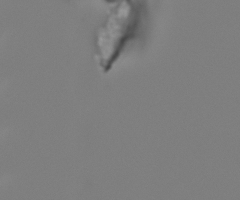
\includegraphics[width=\textwidth]{thesis-template-master/images/(1095).png}
			\caption{Debris}
			\label{fig:Debris}
		\end{subfigure}
		\begin{subfigure}[b]{0.33\textwidth}
			\reflectbox{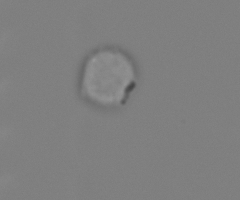
\includegraphics[width=\textwidth]{thesis-template-master/images/(635).png}}
			\caption{Out of Focus}
			\label{fig:Out of Focus}
		\end{subfigure}
		\begin{subfigure}[b]{0.33\textwidth}
			\reflectbox{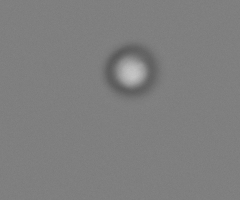
\includegraphics[width=\textwidth]{thesis-template-master/images/(1672).png}}
			\caption{Lighting Artifacts}
			\label{fig:Lighting Artifacts}
		\end{subfigure}
		\begin{subfigure}[b]{0.33\textwidth}
			\reflectbox{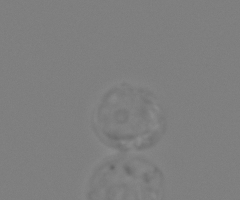
\includegraphics[width=\textwidth]{thesis-template-master/images/(1112).png}}
			\caption{Outside FOV}
			\label{fig:Outside FOV}
		\end{subfigure}
		\begin{subfigure}[b]{0.33\textwidth}
			\reflectbox{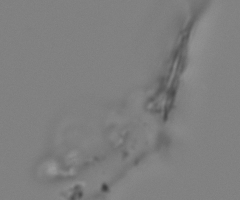
\includegraphics[width=\textwidth]{thesis-template-master/images/(1684).png}}
			\caption{Contaminated}
			\label{fig:Contaminated}
		\end{subfigure}
		\begin{subfigure}[b]{0.33\textwidth}
			\reflectbox{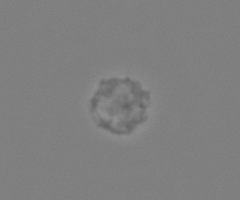
\includegraphics[width=\textwidth]{thesis-template-master/images/hd3 (56).png}}
			\caption{Good Cell}
			\label{fig:Good Cell}
		\end{subfigure}
	\end{center}
	\caption{\textbf{Typical Cell images on the original Sezary Syndrome data set}. Only Good Cell can provide useful Morphology characteristics for further classification.}
	\label{fig:1.1}
\end{figure}

Sezary Syndrom is an aggressive form of cutaneous T-cell lymphoma characterized by the presence of tumor T-cells with abnormal nucleus morphology in the peripheral blood. The smooth and precise detection of malignant cells in the blood of patients with Sezary Syndrome is of significant diagnostic, prognostic, and therapeutic value. It is essential for disease monitoring under treatment\cite{6}\cite{7}. The severe limitations of manual microscopic identification of tumor T-cells have led to the implementation of flow cytometry-based diagnostic assays. Currently, the loss of cell surface markers, such as CD26, CD27, and CD7, on malignant T lymphocytes remains one of the most consistent features and is routinely used in the diagnostic workup \cite{12}. However, their specificity and especially sensitivity must be interpreted with caution \cite{11}. We plan to circumvent the challenges involving the definition of molecular diagnostic markers and instead aim at re-surging a morphology-based diagnosis of hematological malignancies through an automated procedure, integrating imaging flow cytometry and deep learning as a route to, ultra-high throughput and sensitive diagnosis.
 
\label{sub:figures}
\begin{figure}[ht]
	\begin{center}
	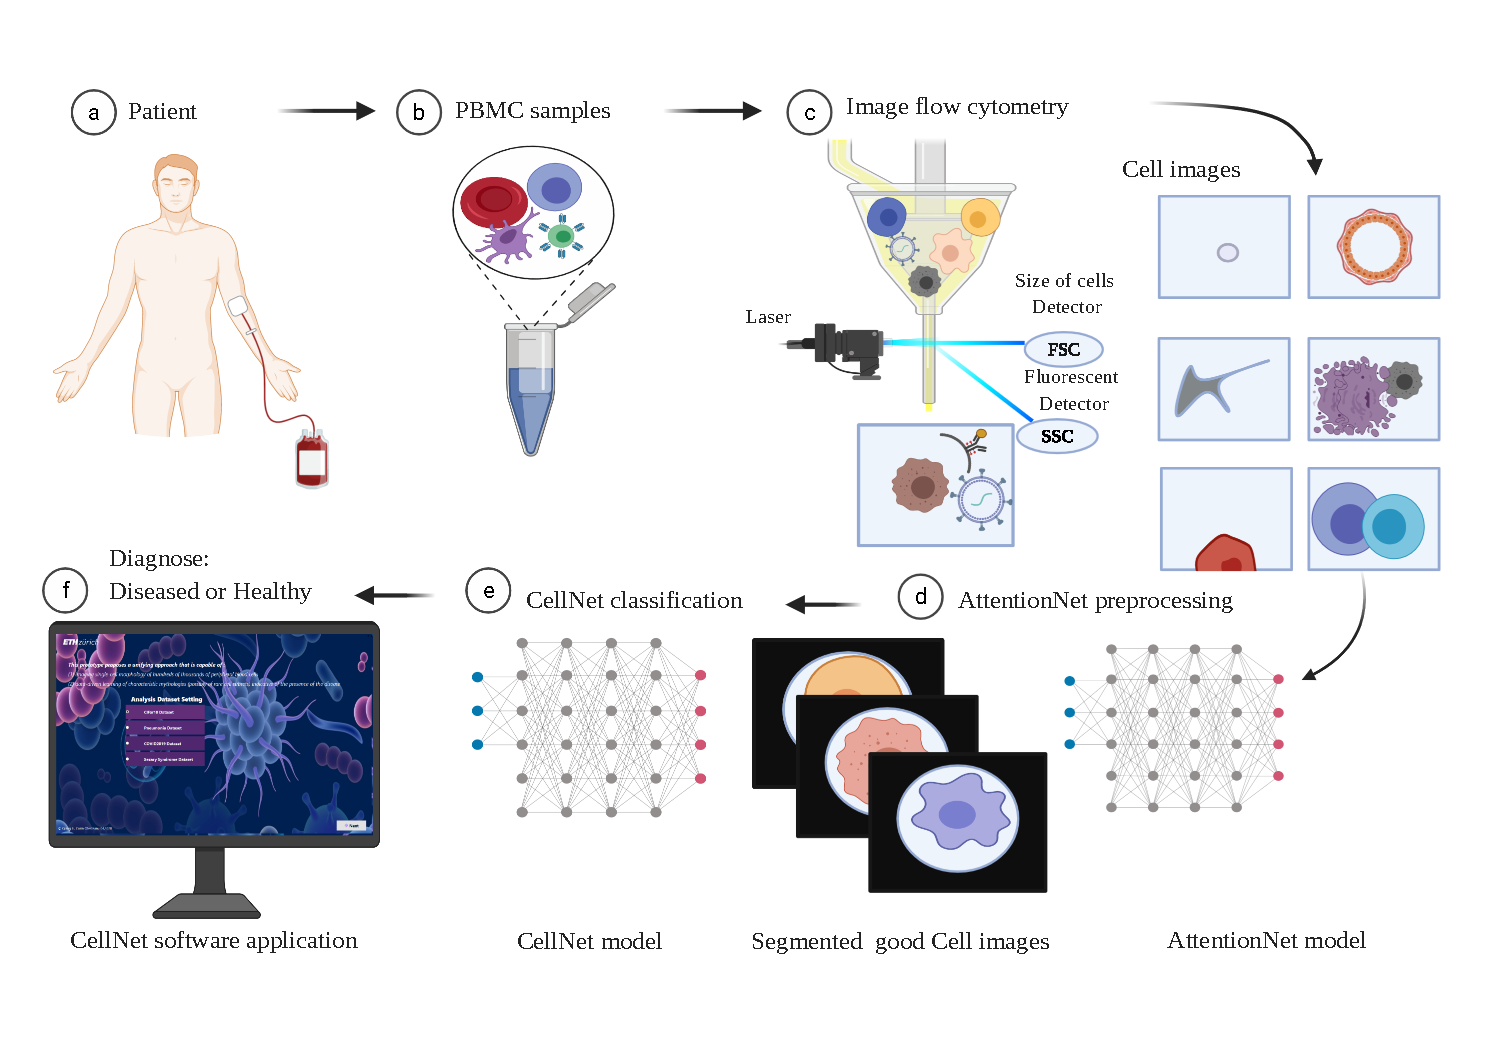
\includegraphics[width=\textwidth]{thesis-template-master/images/general workflow2.pdf}
	\label{fig:lenna}
	\end{center}
	\caption{\textbf{General Workflow of the Proposed Project}. After Image Flow Cytometry (Morphological identification of tumor T-cells in the blood), we can categorize those generated images into six typical classes: lighting artifacts, out of focus cell, debris, contaminated cell, outside FOV cells and multiple cells concatenated together. Using AttentionNet as an automatic detector and segment-or, we can filter out most artifacts in the images and only keep the morphological characteristics of the cell for CellNet classification. CellNet only has eight new Ghost module layers. CellNet software includes a total of 5 interfaces, 25 buttons, ten user prompt functions, and inherits 12 algorithms with the integration of 4 data sets.}
	\label{fig:1.2}
\end{figure}



In the first step, we develop the AttentionNet approach to automatically annotate and segment cell types to single-cell images obtained from imaging flow cytometry experiments. This approach is based on deep learning paradigms that have emerged as a disruptive alternative to engineering-based techniques, which quickly lead to a large amount of raw labeled data, and requires more resources and time. AttentionNet, as an efficient and accurate object detector emphasizing a small target, inherited the characteristics of the real-time detection of the YOLO network\cite{yolov1}, while avoiding the low accuracy of the YOLO network in detecting small objects. Inspired by the YOLOv3-tiny network\cite{33}, the K Means++ algorithm is an efficient approach of data pre-processing\cite{18}. Experimental results demonstrate that AttentionNet is a cost-efficient solution for practical application( Labeling/Segmenting each image takes only 0.25 seconds in Intel CPU) but also an effective way of improving the accuracy of object classification. We reproduced and integrated nearly 20 classic computer vision algorithms and tested it with/without AttentionNet preprocessing. With the help of AttentionNet preprocessing, the improvement based on state-of-the-art algorithms in terms of Top-1 Val-acc has been verified.

Once segmented, we proposed CellNet for Sezary Syndrom Cell / Healthy Cell classification. We applied a similar Residual layer to forward and enable a deeper neural network and follows the basic architecture of ResNet18 and GhostNet for its superiority \cite{19}\cite{20}. Replaced all the ResNet18 \cite{20} point-wise convolutional layers (in total, 18 layers ) with Ghost Bottleneck \cite{19}. Besides, we adopted the SE layers from Squeeze-and-Excitation Networks \cite{24} to enhance useful features, scaling less inhibiting features map. In each ghost module, we first take point-wise convolution to get a few intrinsic feature maps. We utilized the cheap linear transformation such as depth-wise convolution or affine transformation and wavelet transformation, as suggested by GhostNet\cite{19}, here the depth-wise convolution was used.
Despite its simplicity (only 8 layers ghost module) and lower parameters(1/4 weights than ResNet18\cite{20}, 1/2 weights than GhostNet\cite{19}), CellNet establishes a new state-of-the-art on Sezary Syndrome Dataset (95.638\% Top-1 accuracy) and CIFar10 ( 90.051\% Top-1 accuracy)\cite{21}. Moreover, the same method is also very competitive against recent leading Supervised approaches on Pneumonia Dataset (91.785\% Top -1 accuracy), where Inception V3 adopted after 7000 epochs reach only 88.0\%\cite{38}.

The remaining sections of this thesis are organized as follows: Chapter 2 outlines some of the most relevant prior work in medical image classification and segmentation, including a short introduction about YOLOv3 \cite{33} algorithm, an essential intuition of Residual learning, and recently the invention of Ghost module.
Chapter 3 introduces our proposal. Chapter 4 presents experimental verification and visualization on different benchmark datasets to validate the proposed models' effectiveness and illustrates several ablative studies. Finally, conclusions are summarized in Chapter 5.

Our contributions. We propose a unifying approach that is capable of (1) imaging single-cell morphology of thousands of peripheral blood cells and (2) data-driven learning of morphological characteristics, which are indicative of the presence of the disease.
Inspired by the leading SOTA model, such as Deep Residual Learning\cite{20} and Ghosts Net\cite{19}, we proposed CellNet. Instead of stacking lots of point-wise convolutional layers and takes a huge amount of convolutional manipulations, we can avoid the redundant feature maps by taking cheap operation. CellNet is originally designed for Sezary Syndrome Dataset, and we provide comprehensive empirical evidence showing that CellNet has 1/4 weights than ResNet18 \cite{20} and best classification performances on 
several other benchmarks such as CIFar10 \cite{21} (92.451\% Top-1 accuracy), Pneumonia Dataset\cite{38} (91.785\% Top-1 accuracy) and Sezary Syndrome Dataset (95.638\% Top-1 accuracy).
In addition, we proposed AttentionNet Network as an automated data pre-processing tool that provides a new intuition for object recognition; eliminating noise artifacts out of the image precisely can effectively improve the classification performance of many SOTA networks. Instead of manually labeling a large amount of data after Image flow cytometry and PBMC samples \cite{12}, it is possible to automatically label an object with an accuracy of 88.64 \% in 0.25 seconds by using AttentionNet. 

We also produced the first COVID-19 Chest Xray/CT Dataset containing nearly 2,000 Xray/CT images (approximately 1,500 Healthy Xray/CT images and almost 500 COVID-19 infected Xray/CT images). Experiments conducted on COVID-19 Datasets also demonstrated that the proposed CellNet is an effective alternative of current baseline models, and our CellNet (94.719\% in Top-1 accuracy) outperforms the GhostNet\cite{19} (92.739\%  in Top -1 accuracy) and other leading models. We also developed a software application for potential diagnosis, which integrated with 12 leading SOTA models, including our CellNet. All code is available at \textit{https://github.com/Johnny-liqiang/CellNetUML}.

%3D data representations have been studied independently in their main field of application so far. In this thesis, however, we explore the potential of combining geodesic and Euclidean convolutions on point clouds and meshes simultaneously in the task of 3D semantic scene segmentation. In Figure 1.2, we illustrate our intuition that geodesic and Euclidean convolutions focus on different aspects of feature learning. Geodesic convolutions define proximity in terms of mesh neighbors reach￾able within  hops on the mesh. When applying convolutions on this neighborhood, we explicitly learn features focusing on the surface structure of the scene. For instance,in Figure 1.2a, the geodesic receptive field of the green center point just comprises vertices of the geodesically close chair surface. It therefore neglects geodesically remote but spatially close vertices of the table. Hence, we assume that geodesic convolutions are more likely to learn feature representations for object shapes.

%Contrastingly, Euclidean convolutions focus on the Euclidean proximity of vertices in terms of nn or radius neighborhoods in 3D space. They enable an information flow between geodesically disconnected parts of the scene and therefore, we assume that they learn the interaction between objects. For example, in Figure 1.2b, the convolution does not generate features only based on vertices of the chair but also based on the geodesically remote table. We assume that this contextual information helps to distinguish shape-wise similar classes such as chair and armchair. Concludingly, we pose the question if a combination of geodesic and Euclidean convolutions brings a significant benefit for the task of 3D scene segmentation. For this purpose, we have developed a simple yet effective multi-scale architecture called DualConvNet which combines Euclidean and geodesic convolutions in a parallel manner over multiple scales. Special provisions have been taken to guarantee the modularity of the architecture such that all effects are measurable in order to answer the research question in the ablation study experimentally.

%Our approach is mesh-centric in that sense that it consumes meshes as a half-edge data structure as well as defining (un-)pooling operations in terms of mesh simplification algorithms. This design decision is necessary to ensure a mesh structure in deeper network layers such that geodesic convolutions are well-defined. We therefore extend vertex clustering [RB93] and Quadric Error Metrics (QEM) [GH97] as two well-established algorithms from the geometry processing domain such that they can pool and unpool vertex sets from consecutive hierarchy levels. Pooling Trace Maps constitute this extension which comprises a look-up dictionary approach for obtaining pooled representatives in constant time. In order to make QEM pooling applicable for large-scale meshes, we finally present a novel sampling strategy for radius neighborhoods called Random Edge Sampling (RES) which outputs a sample set which guarantees an upper limit of a predefined expected sample size. In the ablation study, we take a closer look at the properties of RES.

%We empirically evaluate our proposed DualConvNet architecture on three publicly available benchmarks for 3D scene segmentation. We achieve competitive results on the ScanNet v2 [DCS+17], as well as the Stanford Large-Scale 3D Indoor Spaces Dataset (S3DIS) [ASZ+16]. Among graph convolutional approaches, we define a new stateof-the-art on both datasets. Moreover, on the recently published Matterport3D benchmark [CDF+17], we can report overall state-of-the-art results. We summarize the main contributions of this thesis as follows: 1 DualConvNet - our novel family of multiscale convolutional architectures - combines Euclidean and geodesic features for 3D semantic scene segmentation. 2 For creating mesh-centric multi-scale architectures, we extend two well-established mesh simplification algorithms as means of (un-)pooling operations. 3 Random Edge Sampling (RES) is a novel sampling method for sampling neighborhoods which guarantees an upper limit for the predefined expected size.
%Reducing the size of the neighborhood allows us to train networks with substantially fewer neighborhood sizes. However, we infer on test examples with larger sample sizes for better neighborhood approximations. 4 We conclude our work with a thorough ablation study which experimentally proves our claim that Euclidean and geodesic convolutions give a consistent benefit, independent of the pooling method and the notion of the neighborhood used in the architecture.

\begin{comment}
\chapter{Related Work}
\label{sec:examples}
This chapter will demonstrate some fun \LaTeX\ stuff.

\subsection[Awesome Figures in the TOC]{Awesome Figures} % (fold)

\label{sub:figures}
\begin{figure}[ht]
	\begin{center}
		\begin{subfigure}[b]{0.49\textwidth}
			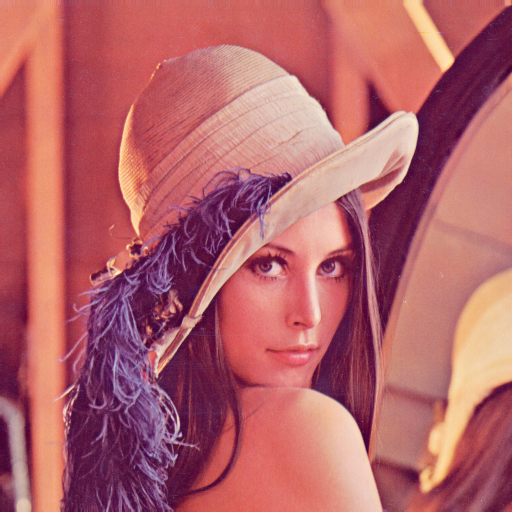
\includegraphics[width=\textwidth]{thesis-template-master/images/lenna.png}
			\caption{Lenna}
			\label{fig:lenna}
		\end{subfigure}
		\begin{subfigure}[b]{0.49\textwidth}
			\reflectbox{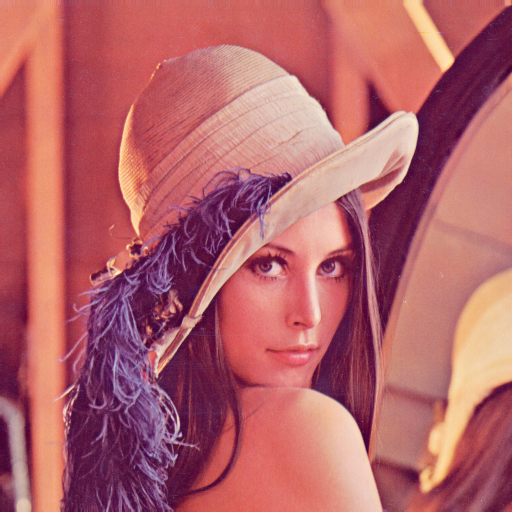
\includegraphics[width=\textwidth]{thesis-template-master/images/lenna.png}}
			\caption{Lenna facing left}
			\label{fig:lenna_facing_left}
		\end{subfigure}
	\end{center}
	\caption{The famous Lenna image used in Computer Vision with subcaptions and a global caption.}
	\label{fig:lennas}
\end{figure}
The figure can be referenced in the text \eg\reffig{lennas}.
Also the subfigures can be referenced \eg\reffig{lenna}, \reffig{lenna_facing_left}.
% subsection figures (end)

\subsection{Citations} % (fold)
\label{sub:citations}
You can cite books from your bibliography \texttt{thesis.bib} (\eg \cite{cochrane}).
Abbreviations from \texttt{abbrev.bib} help in writing the entries.
% subsection citations (end)

\subsection{FixMe warnings}
\label{sub:fixme}
You can add warnings\fxwarning{WARNING} or notifications\fxnote{Note} to your text.
This will help you keep an overview on the places in the text you have to work on.

\section{Lorem}
\label{sec:lorem}


\section{Ipsum}
\label{sec:ipsum}

\subsection{Dolor sit} % (fold)
\label{sub:dolor_sit}


\subsection{Amet} % (fold)
\label{sub:amet}

\end{comment}






\chapter{Related Work}

\section{Learning on Sezary Syndrome}
\subsection{ The introduction of Sezary Syndrome } % (fold)
Sezary Syndrom is an aggressive cutaneous T cell lymphoma characterized by the presence of tumor T cells with abnormal nucleus morphology in the peripheral blood. The smooth and precise detection of malignant cells in the blood of patients with SS is of significant diagnostic, prognostic, and therapeutic value and is essential for disease monitoring under treatment \cite{6}\cite{7}\cite{weng}.

Morphological identification of tumor T cells in the blood is still the gold standard. However, this method is highly subjective, with low throughput and low sensitivity. It also poses severe technical problems, which have not been validated in a multicentre prospective international study \cite{15}. The severe limitations of manual microscopic identification of tumor T cells have fed to the implementation of flow cytometry-based diagnostic assays. Currently, the loss of cell surface markers, such as CD26, CD27, and CD7, on malignant T lymphocytes remains one of the most consistent features and is routinely used in the diagnostic workup \cite{12}. However, their specificity and especially sensitivity must be interpreted with caution \cite{nagler}. A ubiquitously expressed, single clear-cut diagnostic marker allowing for the diagnosis of cutaneous T-cell lymphoma is yet to be discovered \cite{desimone}.


\subsection{ Diagnosis of Sezary Syndrome}

Although Sezary syndrome (SS) outlines as an advanced stage of cutaneous T-cell lymphoma, it is a challenge even for the most experienced dermatologic clinicians. SS is defined clinically by erythroderma, but can also be identified in the presence of specific histologic and peripheral blood findings. Erythrodermic cutaneous T-cell lymphoma can imitate several nonmalignant disorders with erythroderma, including pityriasis rubra pilaris, psoriasis, atopic dermatitis, and graft-versus-host diseases.\cite{nagler}

Because the histology of SS is often nonspecific and rarely pathognomonic, which makes the diagnosis more difficult, peripheral blood studies in patients with erythroderma are usually informative in the diagnosis of SS. Peripheral blood abnormalities consist of elevated CD4/CD8 ratio, aberrant CD26, CD27 and CD7 expression, and T-cell clonality which is helpful for diagnosis \cite{nagler}.

The survey conducted that ratio of CD4: CD8 is often increased in patients with SS, and the clonal proliferation of CD4 cells in CTCL(cutaneous T-cell lymphoma) leads to a CD4: CD8 ratio of 10 or more in  80\% of patients with SS  \cite{nagler-12}. However, the use of the CD4: CD8 ratio for the diagnosis has the shortcomings that patients with benign inflammatory erythroderma have also been found to have ratios that are significantly higher than those of healthy control subjects patients\cite{nagler-13} \cite{nagler-14}.

Besides, an elevated CD4:CD8 ratio is neither sensitive  \cite{nagler-15}  nor specific for CTCL(cutaneous T-cell lymphoma). As a result, the ISCL(International Society of Cutaneous Lymphoma) uses CD4: CD8 greater than ten as a diagnostic criterion for SS, but requires additional hematologic abnormalities \cite{nagler}.    

CD7 is a glycoprotein that is usually exposed in 80\% to 90\% of CD$4 ^{+}$ T cells, virtually all CD$8 ^{+}$T  cells \cite{nagler-15}. CD7 may play a role in T-cell activation and adhesion, but its natural ligand has not been identified \cite{nagler}. CD26 is a glycosylated transmembrane protein that maintains proteolytic enzyme activity (dipeptidyl peptidase IV) and is shown on the majority of circulating T cells and on 80\% to 90\% of CD3 CD4 T cells in the healthy peripheral blood \cite{nagler-28}\cite{nagler-29}. 

\begin{figure}[t]
	\begin{center}
		\begin{subfigure}[b]{0.49\textwidth}
		    \centering
			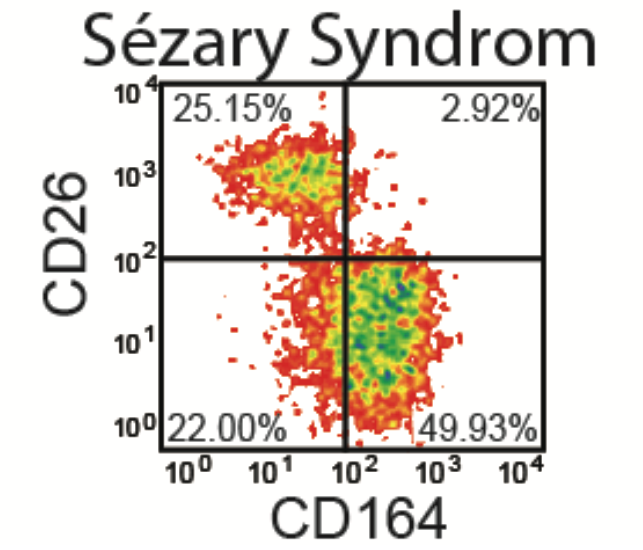
\includegraphics[width=0.8\textwidth]{thesis-template-master/images/cd164.png}
			\label{fig:cellnet}
            \caption{}
		\end{subfigure}
        \begin{subfigure}[b]{0.49\textwidth}
		    \centering
			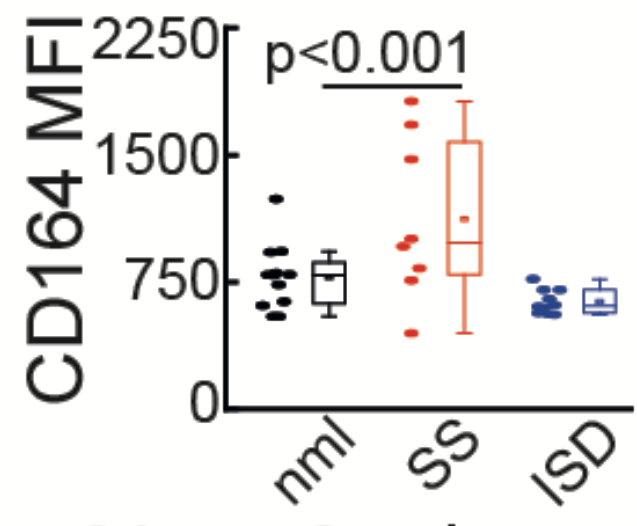
\includegraphics[width=0.8\textwidth]{thesis-template-master/images/sezary and cd164.png}
			\label{fig:cellnet}
            \caption{}
		\end{subfigure}
	\end{center}
	\caption{\textbf{CD164 expression is increased on CD4+ T cells from patients with Sézary syndrome (SS)\cite{emma}}.  Increased expression of CD164 may be a promising diagnostic parameter on Malignant T Cells in Sézary Syndrome, image citated from \cite{emma}
(b) Flow cytometric analysis of CD164 expression in blood CD4+ T cells from healthy donors (nml), control population of patients with inflammatory skin disease (ISD; psoriasis) and patients with SS. (a) Representative example of CD164 expression limited to CD4+ CD26- T cells in the blood of a patient with SS (plot gated on CD4) \cite{emma}.}
    \label{fig:2.1} 
\end{figure}

As shown in \eg\reffig{2.1}, \cite{emma}'s group study was conducted following the declaration of Helsinki's principles and was approved by the Institutional Review Board of the University of Zurich.  They aim to confirm CD164 as a potential marker for malignant T cells in the blood of patients with SS \cite{emma}.

Malignant T cells in CTCL are typically memory T cells. Subsets of memory T cells can be differentiated in part by CD27 expression\cite{nagler-31}\cite{nagler-33}. CD27 belongs to the tumor necrosis factor/nerve growth factor receptor family \cite{nagler}. Although diagnostically invaluable, these peripheral blood studies' diagnostic specificity must be interpreted with caution, particularly when only small numbers of cells are phenotypically abnormal\cite{nagler-6}. Logically, T-cell clonality could be useful in diagnosing SS because neoplasia is the result of a clonal expansion of an abnormal cell\cite{nagler}. However, the diagnostic significance of a dominant T-cell clone in the blood is still controversial, particularly in erythrodermic patients. 

Computer vision approaches have been widely developed to automatically annotate cell types to single-cell images generated from imaging flow cytometry experiments \cite{15}. These approaches are increasingly based on deep learning paradigms that have emerged as a disruptive alternative to engineering-based techniques. Deep learning systems rely on multi-layered neural networks that can extract increasingly complex, task-related features directly from the data. 

Recent developments in neural network architecture design and training have enabled researchers to solve previously intractable learning tasks in the field of computer vision. As a result, deep learning-based approaches have become very successful in addressing a wide range of biomedical image analysis tasks such as detection of skin cancers from photographic images \cite{10}, detection of pneumonia on chest X-rays \cite{13}, detection of breast cancer metastases in histopathology images and many others \cite{2}. 

The above approaches are only limited in deriving a morphological signature in a diagnostic trial since they require a cell type annotation for every single-cell image.

Diagnostic trials provide disease annotations at the level of patient samples that give rise to a collection of single-cell images if processed via imaging flow cytometry, Multiple instance learning (or weakly supervised learning) is an extension of supervised learning that deals with this situation.  In multiple instance learning\cite{5}, disease annotations (e.g., healthy/diseased) are provided for a group of observations (single cell Images) but not for individual observations. Multiple instance learning is particularly appealing for biomedical image analysis, since typically clinical annotations-characterize a group of observations. Multiple instance learning has been successfully applied to cancer detection in histopathology images \cite{8}, where only the whole slide-level information (about presence/absence of cancer in the whole slide) is provided. It has also been applied to the analysis of fluorescence microscopy images from high content screening experiments \cite{9}, where the group label characterizes the majority of cells in the entire microscopy image. 


Recently developed CellCNN \cite{3} for detecting rare diseases, it associates cell populations from single-cell mass cytometry data. CellCnn implements a multiple instance learning approaches to define proteomic profiles of cell subpopulations associated with disease stâtus \cite{3}. Using CellCNN, we identified paracrine signaling-, AlIDS onset- and rare CMV infection-associated cell subsets in peripheral blood and sporadic leukemic blast populations in minimal residual disease-like situations frequencies as low as 0.01\%. CellCNN, in its current form, has been demonstrated on 30+ single-dimensional cell proteomic data and constitutes the basis for our technology prototype to define morphological signatures of disease-associated cell subpopulations from imaging flow cytometry measurements \cite{3}.




\section{Learning on Image Segmentation Techniques }

Here, we learn and compare various techniques for image segmentation techniques. Segmentation based on active contour models conveys that refinement of the boundary was an essential process in segmentation. Grouping of pixels of image conducts for the development of fuzzy-based and K- means clustering method. The kernel metric approaches, in addition to clustering, eliminate the need for prediction number of clusters. K-means based segmentation techniques are applied in various real-world scenarios, such as brain MRI images and tumor segmentation. The Texture Based Encoding Segmentation (TBES) models maintained the reduction of coding length. The uniformity nature of maximum likelihood regions provides a way to use an angular-based texture pattern and intensity deviation matrix to improve the quality of segmentation.\cite{taneja} 

\subsection{ K-Means clustering based Image Segmentation }
The clustering approach assumes that each region in the image forms a separate cluster in the feature space. Those kinds of approaches can be generally divided into two steps: 1) Categorize the points in the feature space into clusters; 2) Map the clusters back to the spatial domain to form separate regions. The most significant advantages led to straight forward for classification and easy for implementation. Under the circumstances of determination of the number of clusters, it will become problematic and usually led to different segmentation results given different initially k clustering centers. Besides, the features are often image dependent, and it remains unclear how to select the best feature set to obtain satisfactory segmentation results. Moreover, it does not benefit from spatial information. 

Recent studies include the local and spatial information in A2DKM to determine the number of clusters and given comparative analysis on memory consumption of AFKM and Automated to Dimensional K means (A2DKM) \cite{A2D}. In \cite{advanced}, they are trying to detect a range of Tumor in brain images and allow accurate detection, reproducible and less execution time, as they mainly work on the brain MR image and use the Tumor shape and Tumor position as evaluation measurement. 

Comparing to Graph-based K-means clustering\cite{graph}, where the application Prim's algorithm and Lloyd algorithm constructs the Minimum Spanning Tree (MST) and generalized cluster centroids to determine the number of clusters and location of cluster centroids \cite{graphmeidan}. Ferrer's studies approved the concept of the generalized median Graph seems to be more adequate to represent the data of each cluster \cite{taneja}.  Given a set of graphs, the generalized median Graph is defined as the Graph that has the minimum sum of distances to all graphs in the set \cite{taneja}. It can be seen as the representative of the set.  For the first time in \cite{graphmeidan}, the use of the generalized median Graph as the representative of a cluster in a graph-based version of the k-means algorithm. 


\subsection{ Level Set based Image Segmentation }
Level set methods consider the topological changes to describe the curves \cite{li18}. The evolving curve in image segmentation stopped at an object boundary by following two ways: applying edge-stopping function and minimization of the energy function \cite{taneja}.

The segmentation process involves more than one-two regions to be segmented. Hence, a multilevel set multi-phase model \cite{li18} included in the level set energy function, and the energy minimization carried out to predict the optimal cluster center and boundary.

The level set formulation utilizes the local criterion function that defines the partition energy for simultaneous image segmentation and analyzes the performance with intensity inhomogeneity \cite{unified}. The Gaussian filter effectively smoothens the initial pixel-wise probabilistic values. Local classifiers and boundary refinement methods are usually used for the effective refinement process \cite{taneja}.

Level set formulation extends the segmentation application to localization of optical disk in retinal images, tracking of non-linear shapes and liver tumor segmentation \cite{taneja} \cite{unified}\cite{li18}. Level set models exclude the information other than the boundary and the intensity inhomogeneity.

\subsection{ Active Contour based Image Segmentation }

The active contour-based image segmentation \cite{unsupervised} utilizes the contour models to carry out the boundary regions. Hence it becomes a critical process in the contour model to obtain a precise segmented boundary with the help of boundary refinement. Here, we briefly go thought three essential techniques used for the boundary refinement analysis: Constrained Active  Contour\cite{constrained}, where boundary refinement tool presented in a constrained active contour for the smooth and accurate boundary; Convex energy function\cite{convex}, where a convex optimization function with local Gaussian distributing fitting term with spatially variations of means and variances presented and the energy function formulated; Unsupervised segmentation \cite{unsupervised}  benefits to segment the protein spots in two-dimensional images with essential issues such as noise, streaks, and multiplets.


\subsection{ Convolutional Networks based Image Segmentation }

The convolutional networks are frequently be applied to classification tasks, producing a single class label of an image. However, especially for biomedical image processing, we are more desired for the output includes localization information,  namely, to assign each pixel a class label \cite{unet}. Moreover, unwell distributed data are more common in biomedical tasks, and small or dirty data problems occur more often. 

Comparing to fully convolutional network, where supplementing a usual contracting network by successive layers and replacing the pooling operators with upsampling operators,  U-net \cite{unet} facing very little training data available, furthermore the separation of touching objects of the same class. To overcome those challenges, the U-net consists of a contracting path (left side) and an expansive path (right side). 

\begin{figure}[t]
\begin{center}
\centering
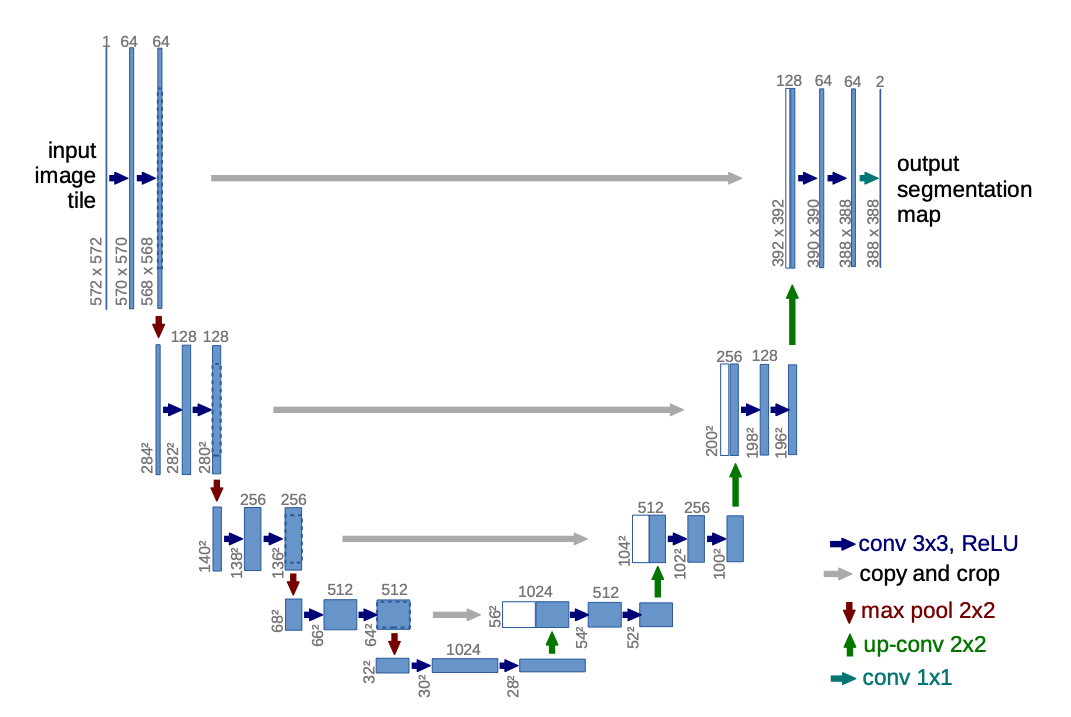
\includegraphics[width=\textwidth]{thesis-template-master/images/unet.png}
\label{fig:cellnet}
\end{center}
\caption{\textbf{U-net architecture (example for 32x32 pixels in the lowest resolution)\cite{unet}}. Each blue box corresponds to a multi-channel feature map. The number of channels is denoted on top of the box. The x-y-size is provided at the lower left edge of the box. White boxes represent copied feature maps. The arrows denote the different operations.}
\label{fig:2.2}
\end{figure}

As shown in \eg\reffig{2.2}, the contracting path follows the typical architecture of a convolutional network to capture context. It consists of the repeated application of two $3\times3$ convolutions (unpadded convolutions), each followed by a rectified linear unit (ReLU) and a $2\times2$ max pooling operation with stride 2 for downsampling \cite{unet}. Every step in the expansive path consists of an upsampling of the feature map followed by a $2\times2$ convolution ("up-convolution") that halves the number of feature channels, a concatenation with the correspondingly cropped feature map from the contracting path, and two $3\times3$ convolutions, each followed by a ReLU\cite{unet}. The expanding path is to enable precise localization.

To overcome small data problems, they generated smooth deformations using random displacement vectors on a coarse 3 by 3 grid on data and elastic deformations to the available training images\cite{unet}. As a result, the U-net outperforms the prior best method (a sliding-window convolutional network) on the ISBI challenge and  won the ISBI cell tracking challenge 2015 in these categories by a large margin \cite{unet}


\section{Learning on YOLO network}

The objective of the You Only Look Once (YOLO)\cite{yolov1} is to identify which of a known set of objects might be present and to localize their positions within the image by giving an image or a video stream. Prior work on object detection repurposes classifiers to perform detection. As a representative object detection model based on regression, You Only Look Once (YOLO) frames object detection as a regression problem to spatially separated bounding boxes and associated class probabilities \cite{yolov1}.

The first version YOLO network\cite{yolov1} divides the image into an $S \times S$ grid ( YOLO chose S=7) and for each grid cell predicts B bounding boxes (YOLO chose B=2), confidence for those boxes, and C class probabilities \cite{yolov1}. Each bounding box consists of 5 predictions: x, y, w, h, and confidence score \cite{yolov1}, which prevents the YOLO from detecting backgrounds.  If there is no object in the cell, the confidence scores should be zero.  Otherwise, the confidence score will be equal to the intersection over union (IOU) between the predicted box and the ground truth. Therefore,  all these predictions are encoded as an $S × S × (B ∗ 5 + C)$ tensor \cite{yolov1}.

If the center of an object falls into a grid cell, that grid cell is responsible for detecting the object. Each grid cell can detect only one object, so in total, we will drive into $7\times 7=49$ grid cells for each image. For each cell, it predicts two boxes (98 boxes in total). The vast majority of these boxes will have shallower confidence and then to get rid of most of them by using NMS \cite{yolov1}.

The reason for using a confidence score equal to the IOU is that we are 100\% sure that there is an object inside the ground truth box, then the higher the IOU, the higher the possibility that an object occurs inside the predicted box.



\begin{figure}[t]
\begin{center}
\centering
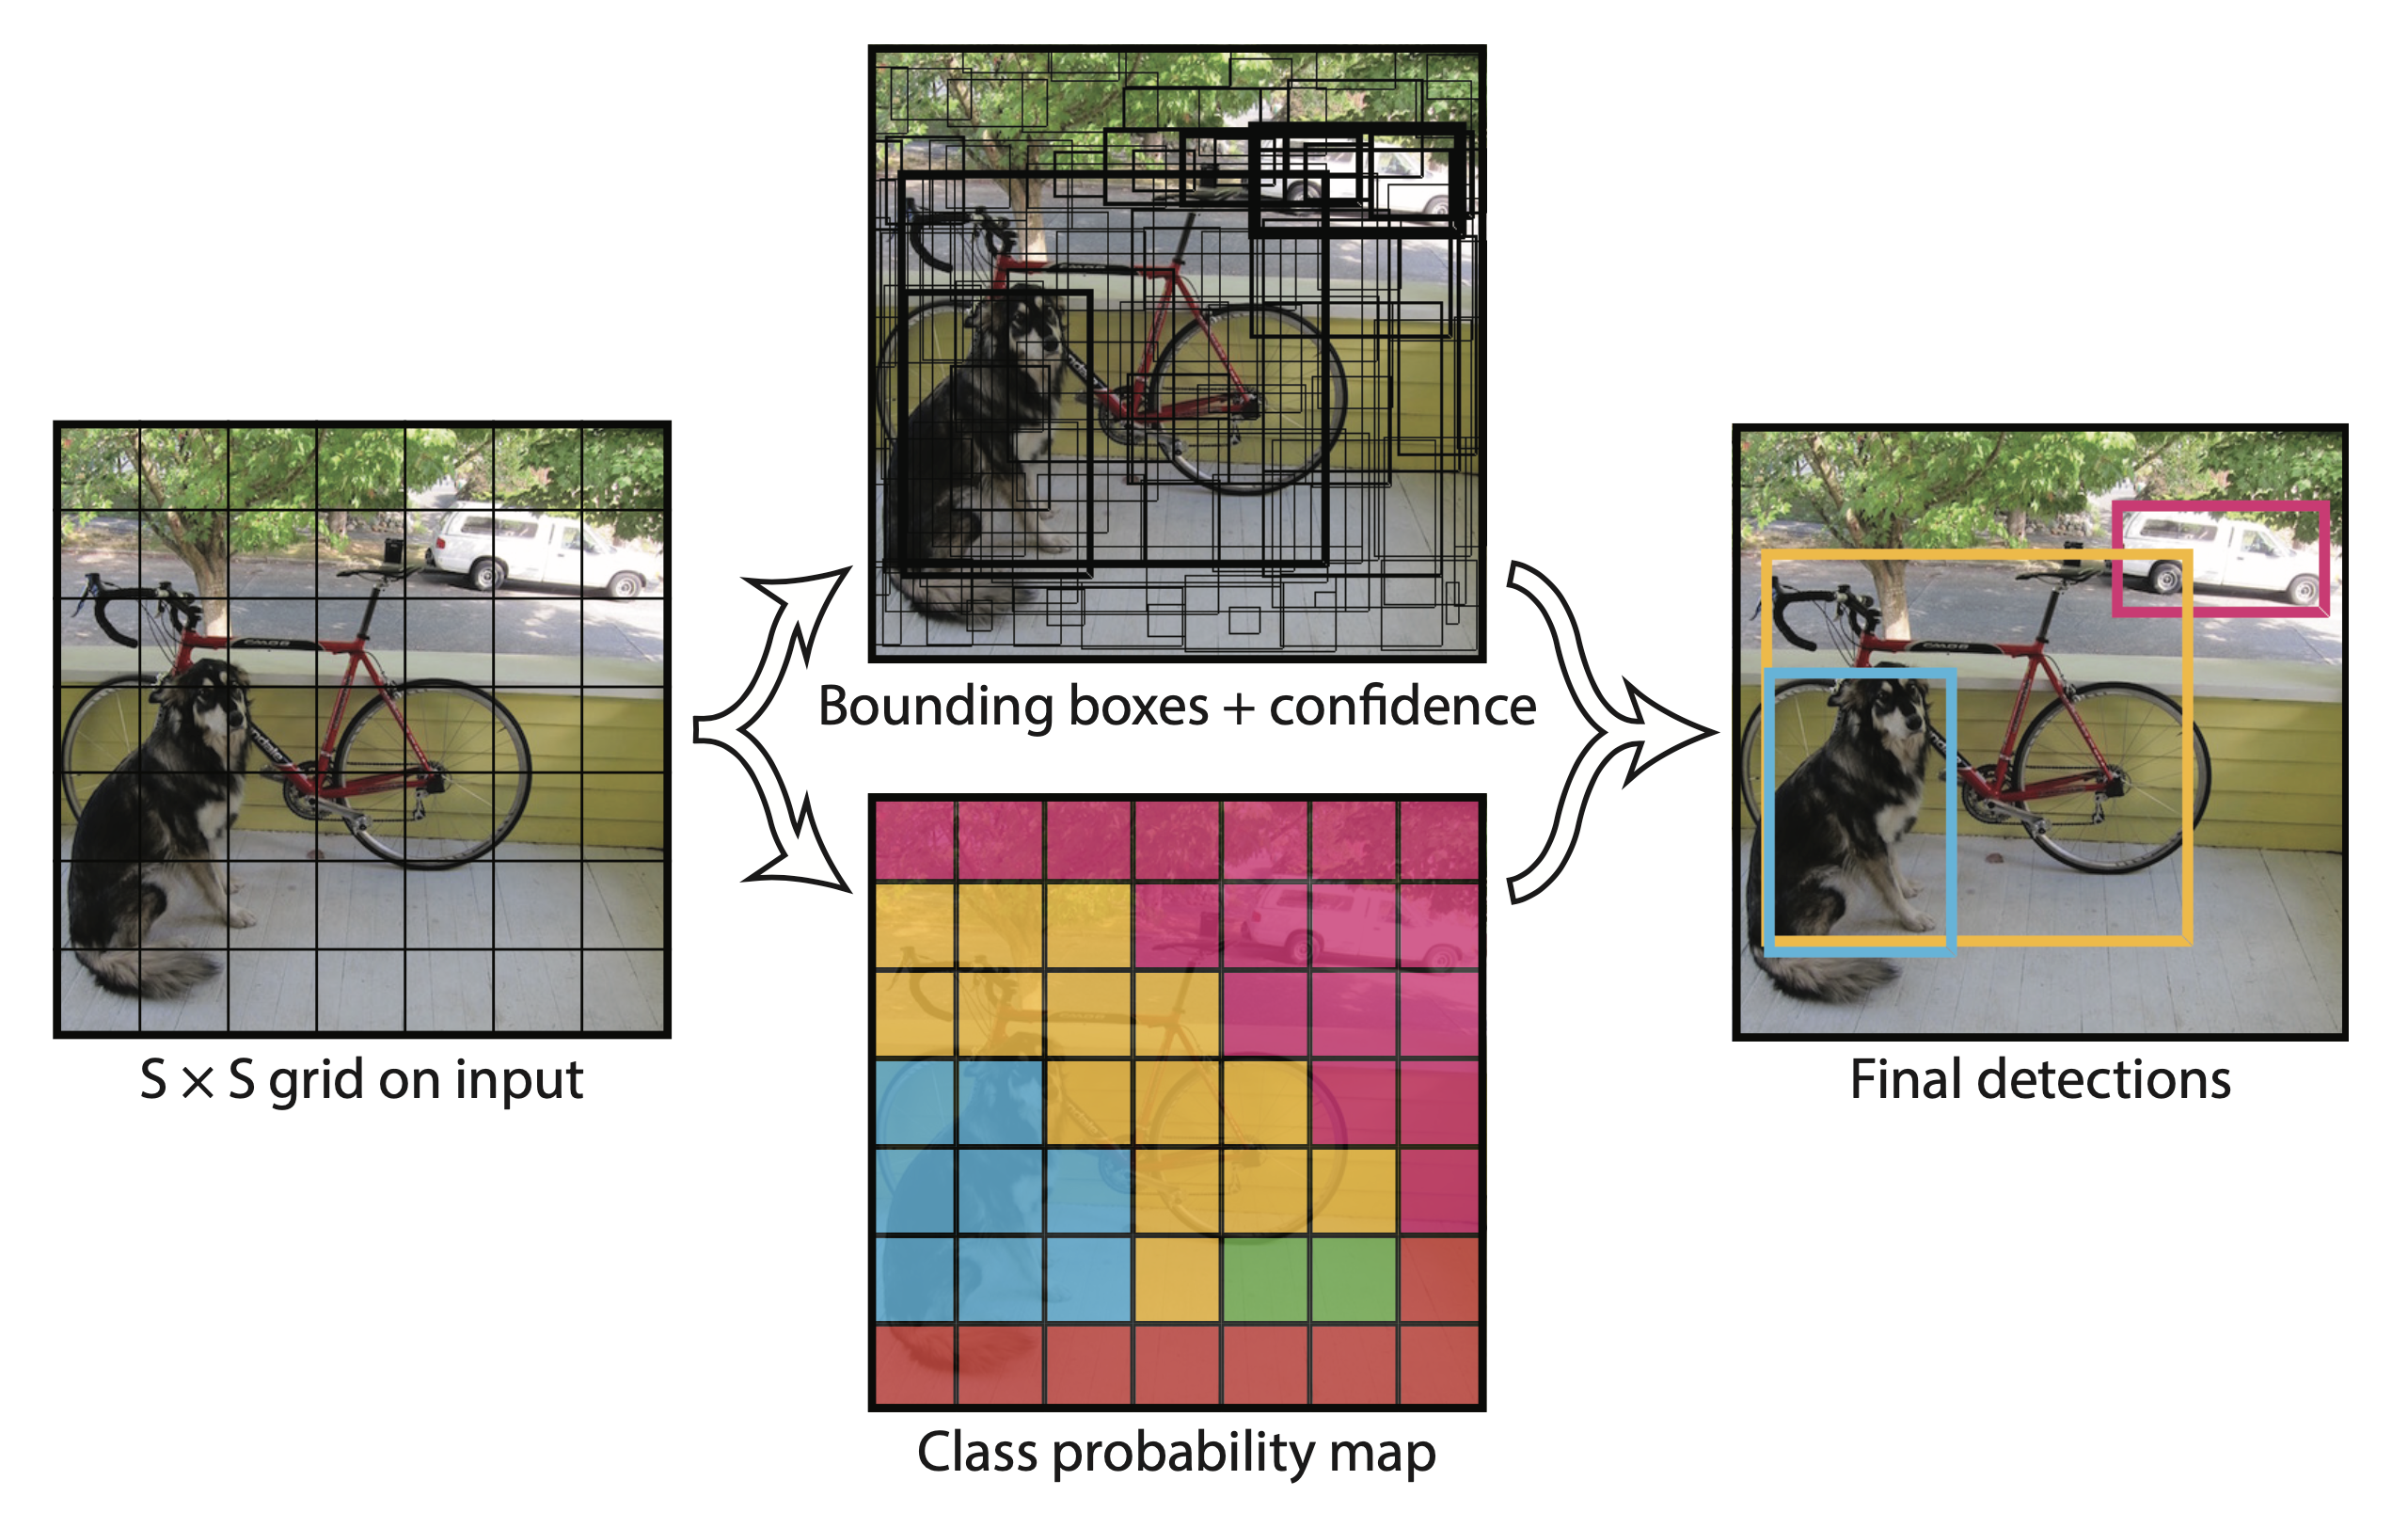
\includegraphics[width=\textwidth]{thesis-template-master/images/yolomodel.png}
\label{fig:cellnet}
\end{center}
\caption{\textbf{YOLO model\cite{yolov1}}. YOLO\cite{yolov1} was trained to detect 20 different classes of objects. For any grid cell the model will calculate 20 conditional class probabilities one for each class, while each grid cell gives us a choice between two bounding boxes. The final detection scores encode both the probability of that class appearing in the box and how well the predicted box fits the object.}
\label{fig:2.3}
\end{figure}


 The original  YOLO network architecture has 24 convolutional layers, followed by two fully connected layers\cite{yolov1}. Instead of the inception modules used by GoogleNet, YOLO uses $1 \times 1 $reduction layers, followed by $3 \times3 $convolutional layers. The final layer predicts both class probabilities and bounding box coordinates.


\subsection{ Real-Time Object Detection }

You only look once (YOLO) predicts object class and location with exceeding fast speed, namely, on a Titan X GPU, its third version can run at 45 frames per second without any batch processing \cite{18}. Furthermore, YOLO achieves a higher mean average precision (mAP) than other real‐time systems. Since the whole detection pipeline is a single network, it can be optimized end-to-end directly on detection performance \cite{18}.

%As a single neural network, YOLO is extremely simple, which can concurrently predict bounding boxes coordinates and associated class probabilities from full images in one evaluation.

To push the boundaries of fast object detection, the  Fast YOLO \cite{yolov1} uses a neural network with fewer convolutional layers (9 instead of 24) and fewer filters in those layers. Some obvious drawbacks lead to Incremental Network Based on YOLO\cite{yolov1}, such as YOLOv2\cite{yolov2}, YOLOv3\cite{33}, TF-YOLO and YOLOv3-Tiny\cite{18}.

Firstly, YOLO\cite{yolov1} prophesies multiple bounding boxes per grid cell. At training time, only one bounding box predictor is responsible for each object, based on which prediction has the highest current IOU with the ground truth. That leads to specialization between the bounding box predictors.

Secondly, since in the first YOLO network, they used $7\times7$ grid, and any grid can detect only one object\cite{yolov1}. The maximum number of objects the model can detect is 49. When a grid cell contains more than one object, the model will not be able to detect all of them is the problem of close object detection that first YOLO suffers from. Those lead to struggles with small objects that appear in groups as well, such as flocks of birds\cite{yolov1}. Furthermore, the first YOLO  learns to predict bounding boxes from pre-trained ImageNet data, and it is not well generalized to objects in new or unusual aspect ratios or configurations\cite{18}. 

Last but not least, loss function applied treats errors the same in small bounding boxes versus large bounding boxes\cite{yolov1}. A small error in a large box is generally benign, but a small error in a small box has a much more significant effect on IOU \cite{yolov1}.



\subsection{ Improved Incremental Network Based on YOLO }


Here, we will go through all the improved incremental networks based on the original YOLO. To eliminate the YOLO's drawbacks on the areas mentioned above, Redmon contributed significantly to YOLOv2 \cite{ yolov2} and YOLOv3 \cite{33} in recent years. 

The original YOLO makes a significant number of localization errors and has a relatively low recall. Thus in the YOLOv2 \cite{ yolov2}, they focus mainly on promoting recall and localization while maintaining classification accuracy. By combining batch normalization on all of the convolutional layers in YOLO,  YOLOv2 perceived more than 2\% improvement in mAP \cite{ yolov2}.

Secondly, YOLOv2  \cite{ yolov2} initially trained the model on images at $224\times224$, then fine tuning the classification network at the full $448\times448$ resolution for ten epochs on ImageNet before training for detection.  It provides the network time to adjust its filters to work better on higher resolution input. This high-resolution classification network produces an increment of nearly 4\% mAP\cite{yolov2}.

In contrast to YOLOv1 \cite{ yolov1} tries to assign the object to the grid cell that holds the core of the object,  YOLOv2 \cite{ yolov2} attempts to allow the grid cell to detect more than one object using  $K$ bounding box. To predict $ K$ bounding boxes, YOLOv2 used the concept of Anchor boxes\cite{ yolov2}, which can predict the bounding box relative to it instead of predicting the box relative to all images.   YOLOv2 assigns the predicted bounding box not only to the grid cell but also to one of the anchor boxes, which has the highest IOU with the ground truth box \cite{yolov2}. 


\begin{figure}[t]
\begin{center}
\centering
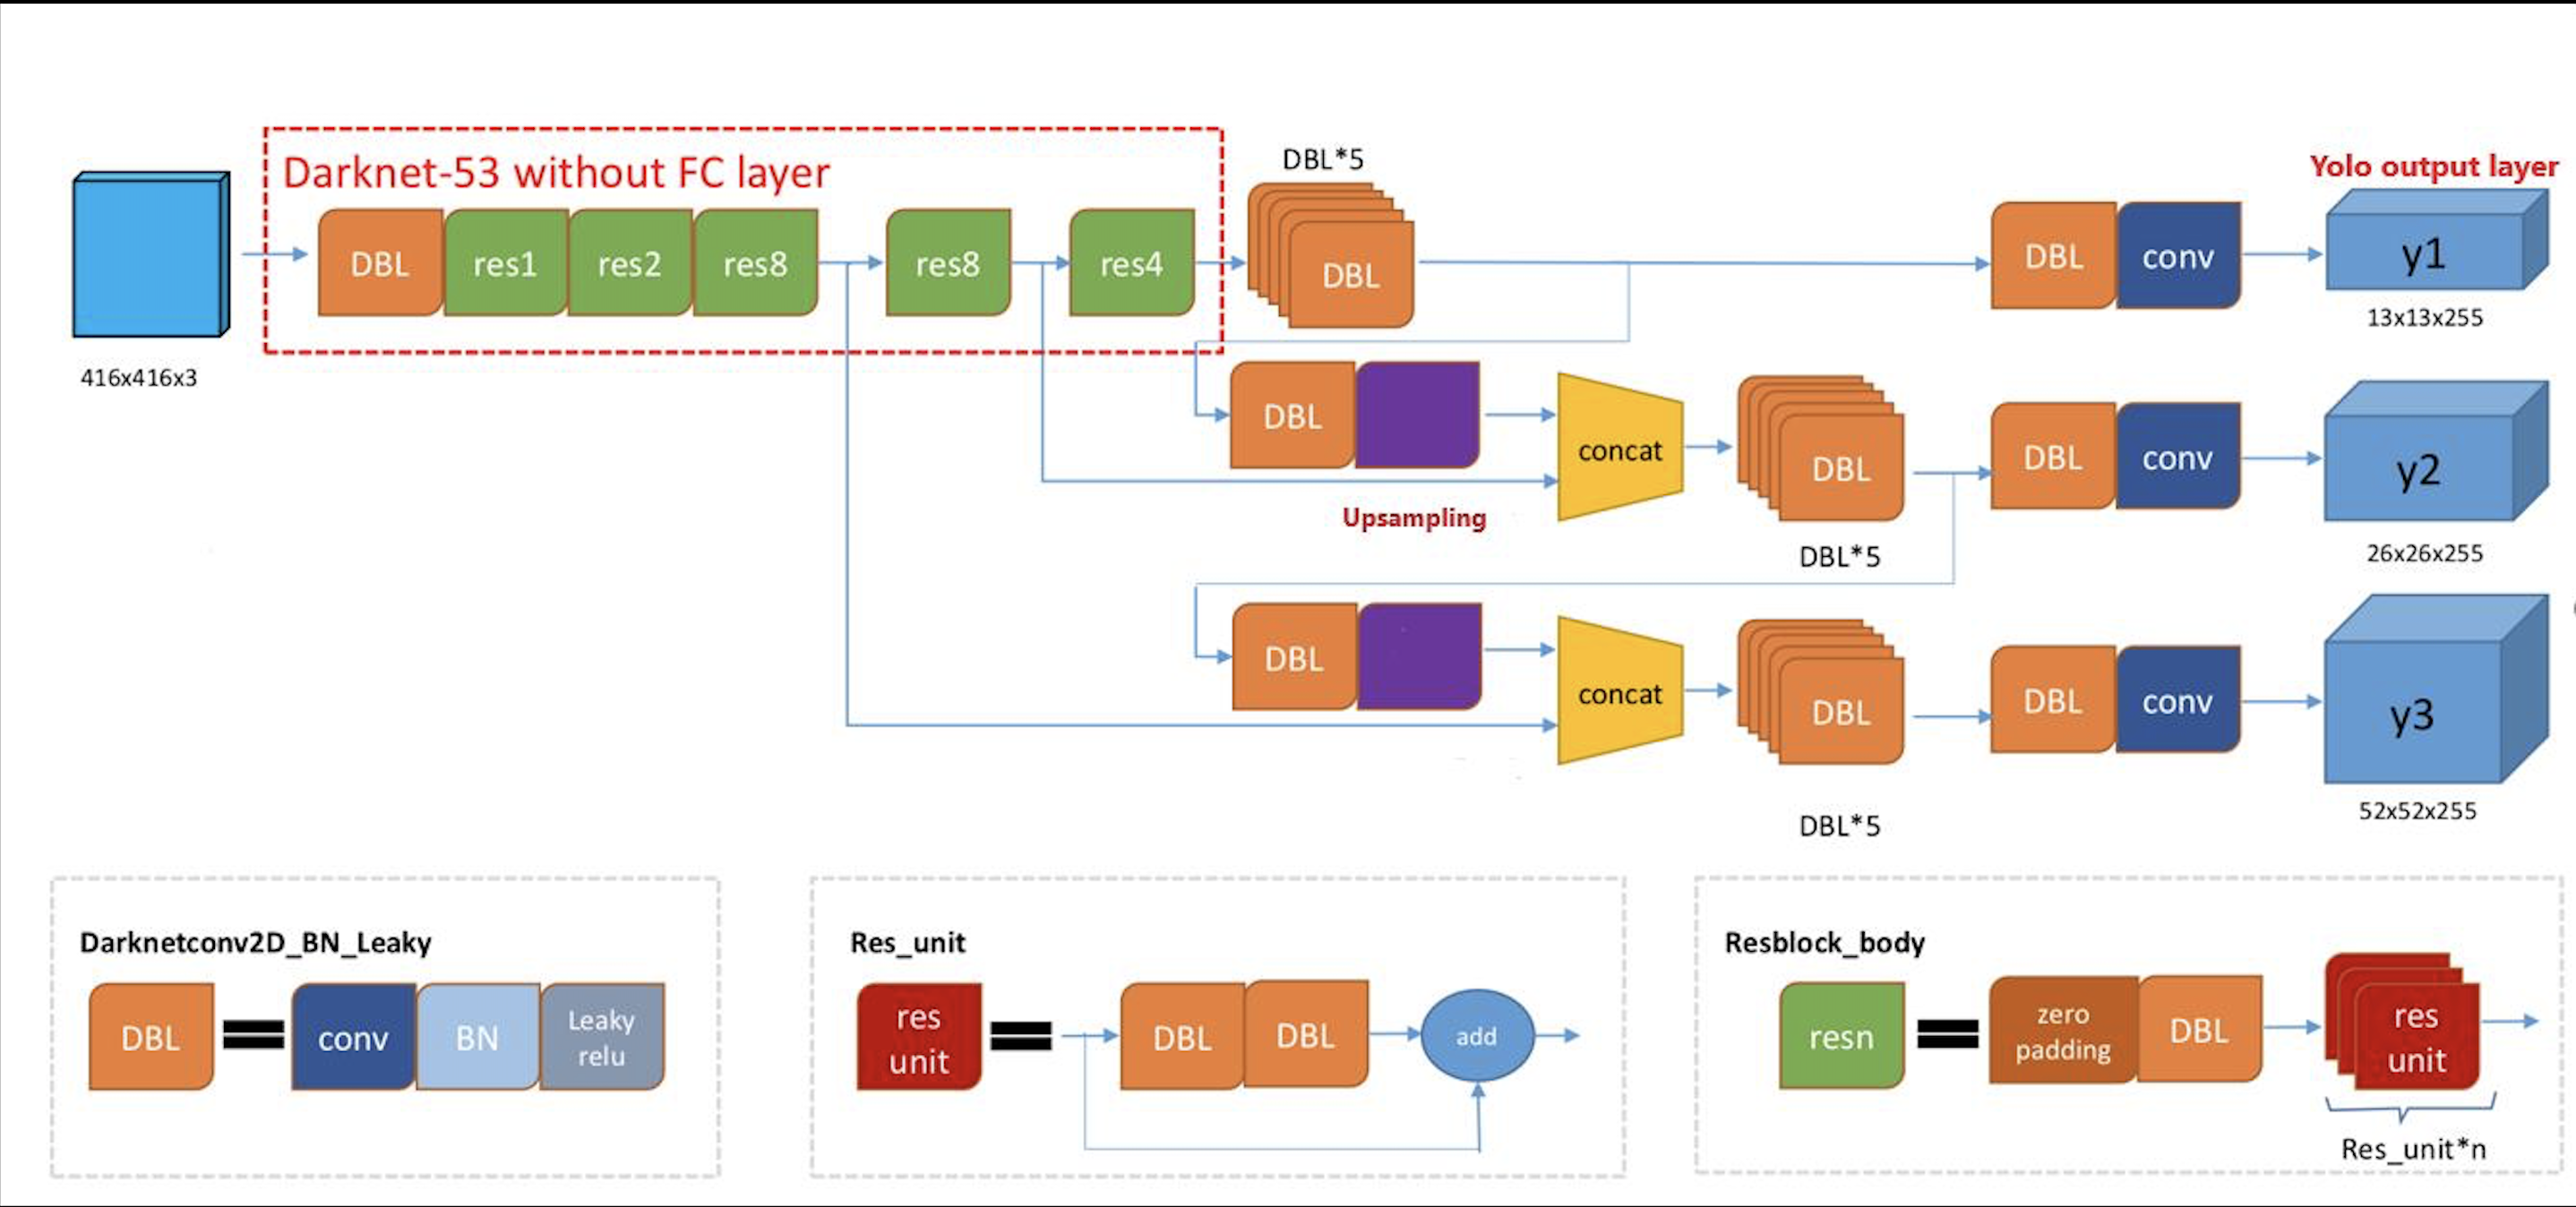
\includegraphics[width=\textwidth]{thesis-template-master/images/yolov3.png}
\label{fig:cellnet}

\end{center}
\caption{\textbf{The architecture of YOLOv3}. YOLOv3\cite{33} follows the principle of the coordinate prediction in YOLOv2\cite{yolov2}, for predicting the categories, multi-label and multi-classification are applied instead of the original single label and multi-classification.}
\label{fig:2.4}
\end{figure}

Using a softmax for class prediction imposes the assumption that each box has precisely only one class. For this reason, YOLOv3 \cite{33} does not use a softmax. It merely uses independent logistic classifiers for any class. Meanwhile, YOLOv3\cite{33} adopts the binary cross-entropy loss function instead of the multi-class loss function. On a standard computer with GPU, it is easy for YOLOv3 to achieve real-time performance \cite{18}.  

Besides, YOLOv3 \cite{33} achieves better performance on small objects by using shortcut connections to get more finer-grained information from the earlier feature map. However comparing to the previous version, YOLOv3 has worse performance on medium and larger size objects \cite{33}.

Moreover, in the miniaturized embedded devices, such as Nvidia SoM, the conventional YOLOv3 algorithm runs slowly\cite{18}. Nevertheless, the YOLOv3-tiny network can better satisfy real-time requirements based on limited hardware resources with comparable accuracy. Therefore we adopted the principle of coordinate prediction in YOLOv3\cite{33} and focused on the improvement of YOLO v3-tiny in this thesis.

\section{Learning on Deep Residual Learning}

Deep residual networks \cite{20} steered the deep learning world when Microsoft Research released a series of ResNets. These networks won 1st-place  in all five main tracks of the ImageNet and COCO 2015 competitions, which embraced image classification, object detection, and semantic segmentation\cite{20}. Various visual recognition tasks and non-visual tasks involving speech and language verified the robustness and superior performance of ResNets. Leading advanced continuing works are proposed based on the concept of residual learning of ResNet\cite{20}.

The baseline of our group's prototype that data-driven learning of characteristic morphologies (possibly of rare cell subsets) indicates the presence of the disease wass based on ResNet18\cite{20}. 
Baseline of diagnosis of Sezary cells can score 91\% top-1 accuracy with 10,000 training images, which consists of 50,000 HD cells and  50,000 SS cells. However, when it applies to test data set when multiple artifacts appear, most of the attention will be dropped in those areas, which leads to a cliff-like decline on accuracy. It is also the core purpose of this thesis: to achieve more robust detection and classification on small objects and data sets full of noise, such as the Sezary Syndrome dataset.


\subsection{ Residual Learning }

In ResNet\cite{20}, they explicitly reformulated residual layers and provided extensive evidence showing that these residual networks can solve degradation problem: when the network depth is increasing, the accuracy gets unsurprising saturated and then degrades rapidly \cite{20}.
More importantly, they evaluated both 18-layer and 34-layer ResNet, and the 34 layer ResNet exhibits considerably lower training error and validation error. The 18-layer ResNet converges much faster while still keep comparable accuracy \cite{20}. 

\begin{figure}[t]
\begin{center}
\centering
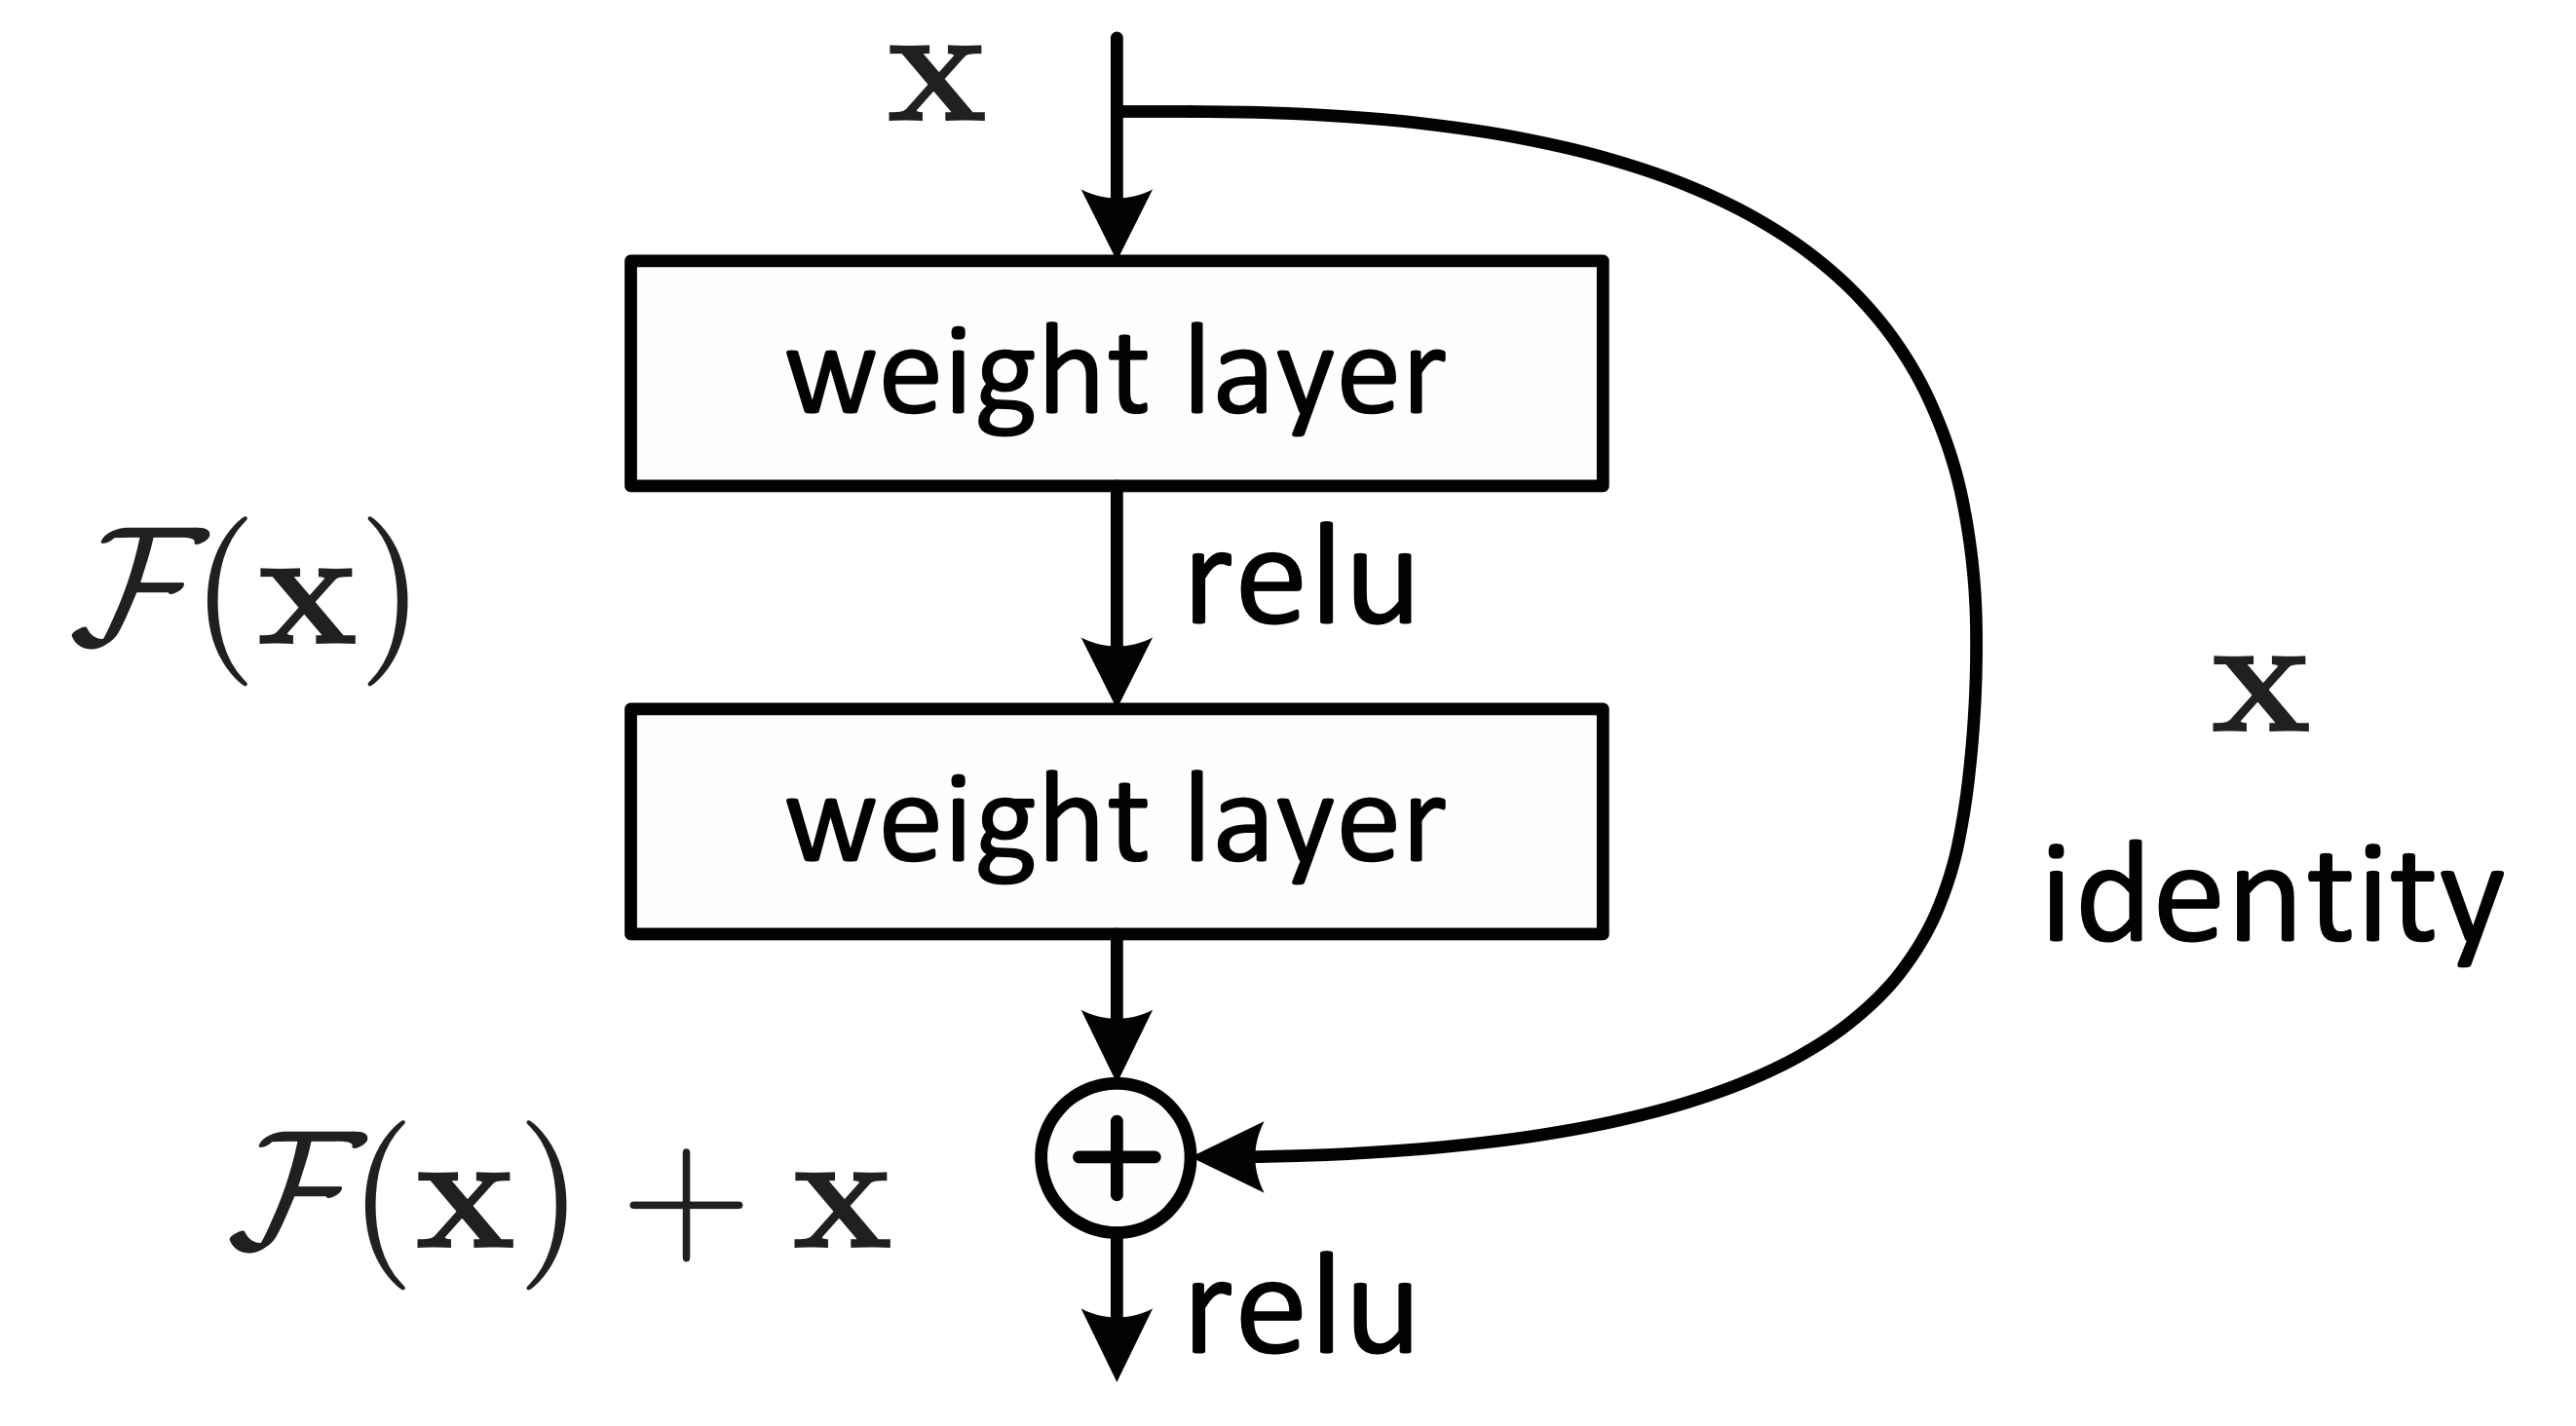
\includegraphics[width=0.7\textwidth]{thesis-template-master/images/RES.png}
\label{fig:cellnet}
\end{center}
\caption{\textbf{Residual learning: a building block \cite{20}}. Identity shortcut connections add neither extra parameter nor computational complexity, but they can easily enjoy accuracy gains from significantly increased depth.}
\label{fig:2.5}
\end{figure}

In a standard residual block \cite{20}, they first performed downsampling with a stride of 2, namely, Convolution, BatchNormalization, and  LeakyReLU have applied accordingly, then Conv2D plus BatchNormalization weight layer is adopted as well. For the third step,identity shortcuts are utilized directly when the input and output are of the same dimensions. Otherwise, when the dimensions increase, they acknowledged two options:  still performs identity mapping with extra zero entries padded for increasing the dimensions; projection shortcut is used to match dimensions (done by 1×1 convolutions). For both options, when the shortcuts cover feature maps of two sizes, they are performed with a stride of 2 \cite{20}.


\subsection{ Variously increment Improvement }

The authors of residual networks\cite{20} tried to make the model as thin as possible in favor of increasing their depth, having fewer parameters, and even introducing a «bottleneck» block, which makes ResNet blocks even thinner. However, as \cite{wideres}  addressed, the diminishing feature reuse problem will occur. \cite{wideres} declared that the main power of deep residual networks is in residual blocks and that the effect of depth is supplementary (contrary to what was believed). Moreover, \cite{stochasticres} investigated the diminishing feature reuse problem with the idea of randomly disabling residual blocks during training, while this method can be viewed as a special case of dropout\cite{dropout}.

\begin{figure}[t]
\begin{center}
\centering
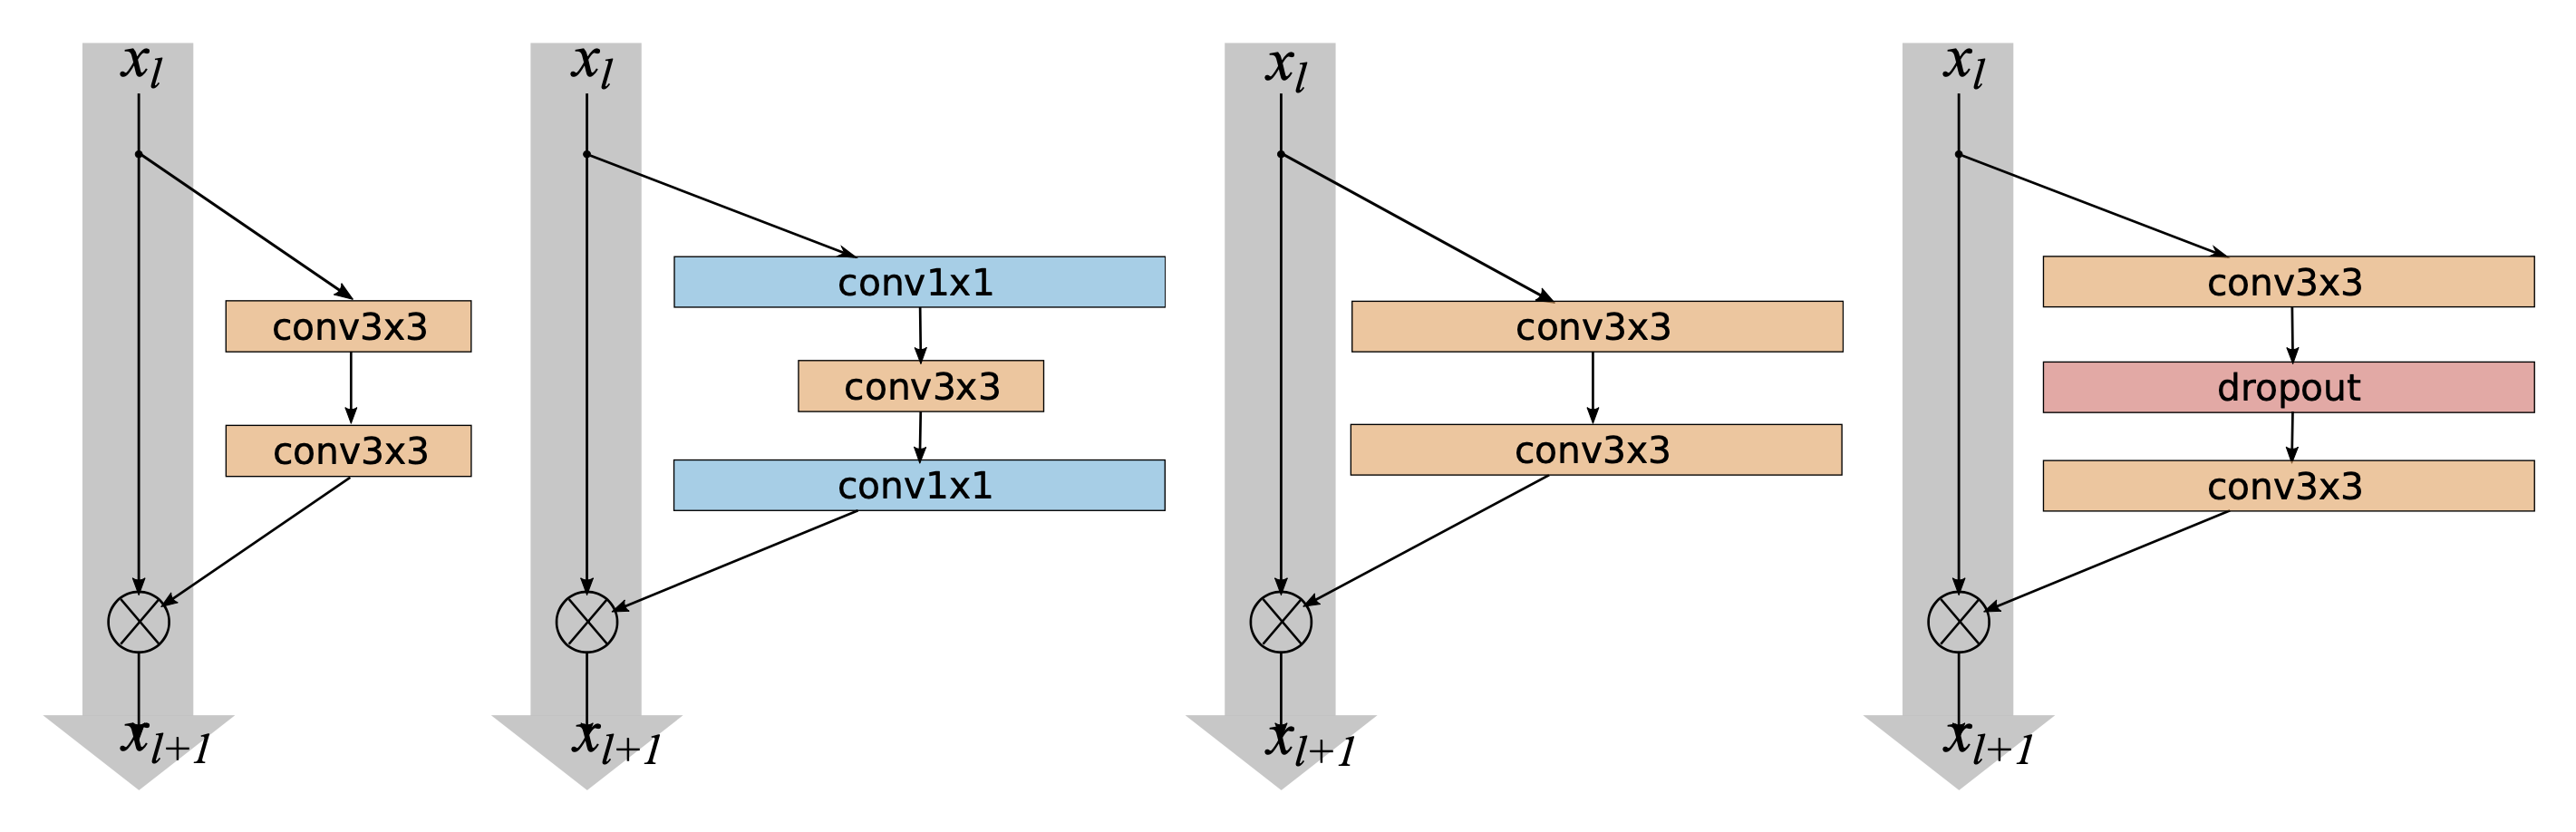
\includegraphics[width=\textwidth]{thesis-template-master/images/wide.png}
\label{fig:cellnet}
\end{center}
\caption{\textbf{Various residual blocks used in \cite{wideres}}. Batch normalization and ReLU precede
each convolution (omitted for clarity).}
\label{fig:2.6}
\end{figure}

Wide (width refers to the number of channels in a layer) residual networks \cite{wideres} attempt to address the problem of diminishing feature reuse in very deep (thin) residual networks, namely, few residual blocks are learning useful representations or many blocks sharing very little information with a small contribution to the final goal, by increasing the model capacity (number of parameters) and adding additional regularization in the form of dropout \cite{dropout}.

In fact, as \eg\reffig{2.6} shows, there is a balance between the depth and width of these networks: if layers are too wide, the model will learn extraneous information (added noise); if layers are too thin,  subsequent layers will not have much to learn from (i.e., diminishing feature reuse).

Aggregated Residual Transformations for Deep Neural Networks \cite{aggres} of Facebook AI Research exposes a new dimension called cardinality as an essential network parameter, in addition to depth and width. Cardinality is demonstrated to be more effective than going deeper or broader when increasing model capacity, especially when increasing depth and width leads to diminishing returns\cite{aggres}.




\section{Learning on Feature Extraction}

The redundancy in feature maps is an essential characteristic of those successful CNNs\cite{20}\cite{wideres}\cite{31}\cite{32}, but has rarely been investigated in neural architecture design. Ghostnet \cite{19}  first proposes a new Ghost module to generate more feature maps from cheap operations. Based on a set of intrinsic feature maps, by applying a series of linear transformations with cheap cost to generate many ghost feature maps that could fully reveal information underlying intrinsic features \cite{19}.

Traditional CNNs usually need a more significant number of parameters and floating-point operations (FLOPs)to achieve satisfactory accuracy,e.g., ResNet-50  \cite{20}
has about 25.6M parameters and requires 4.1B FLOPs to process an image of size $224\times224$.

Experiments conducted on benchmarks demonstrate those successful CNN's \cite{20}\cite{wideres}\cite{31}\cite{32} generated most of the extrated feature maps are similar and can be approximately obtained by transforming each other through cheap operations\cite{19}.

\subsection{ Point-wise Convolution }

The commonly applied feature extraction techniques are convolution, which is precisely the point-wise convolution since the first convolution manipulation was invented and brings the record-breaking performance through various computer vision tasks, such as image recognition, object detection, and semantic segmentation.
However, when the saliency map begins for the understandable CNN and explainable AI, the researcher proposes a series of methods to investigate compact deep neural networks, such as network pruning and low-bit quantization and knowledge distillation to prune the unimportant weights in neural network and achieve higher speed-up ratios.

\begin{figure}[t]
\begin{center}
\centering
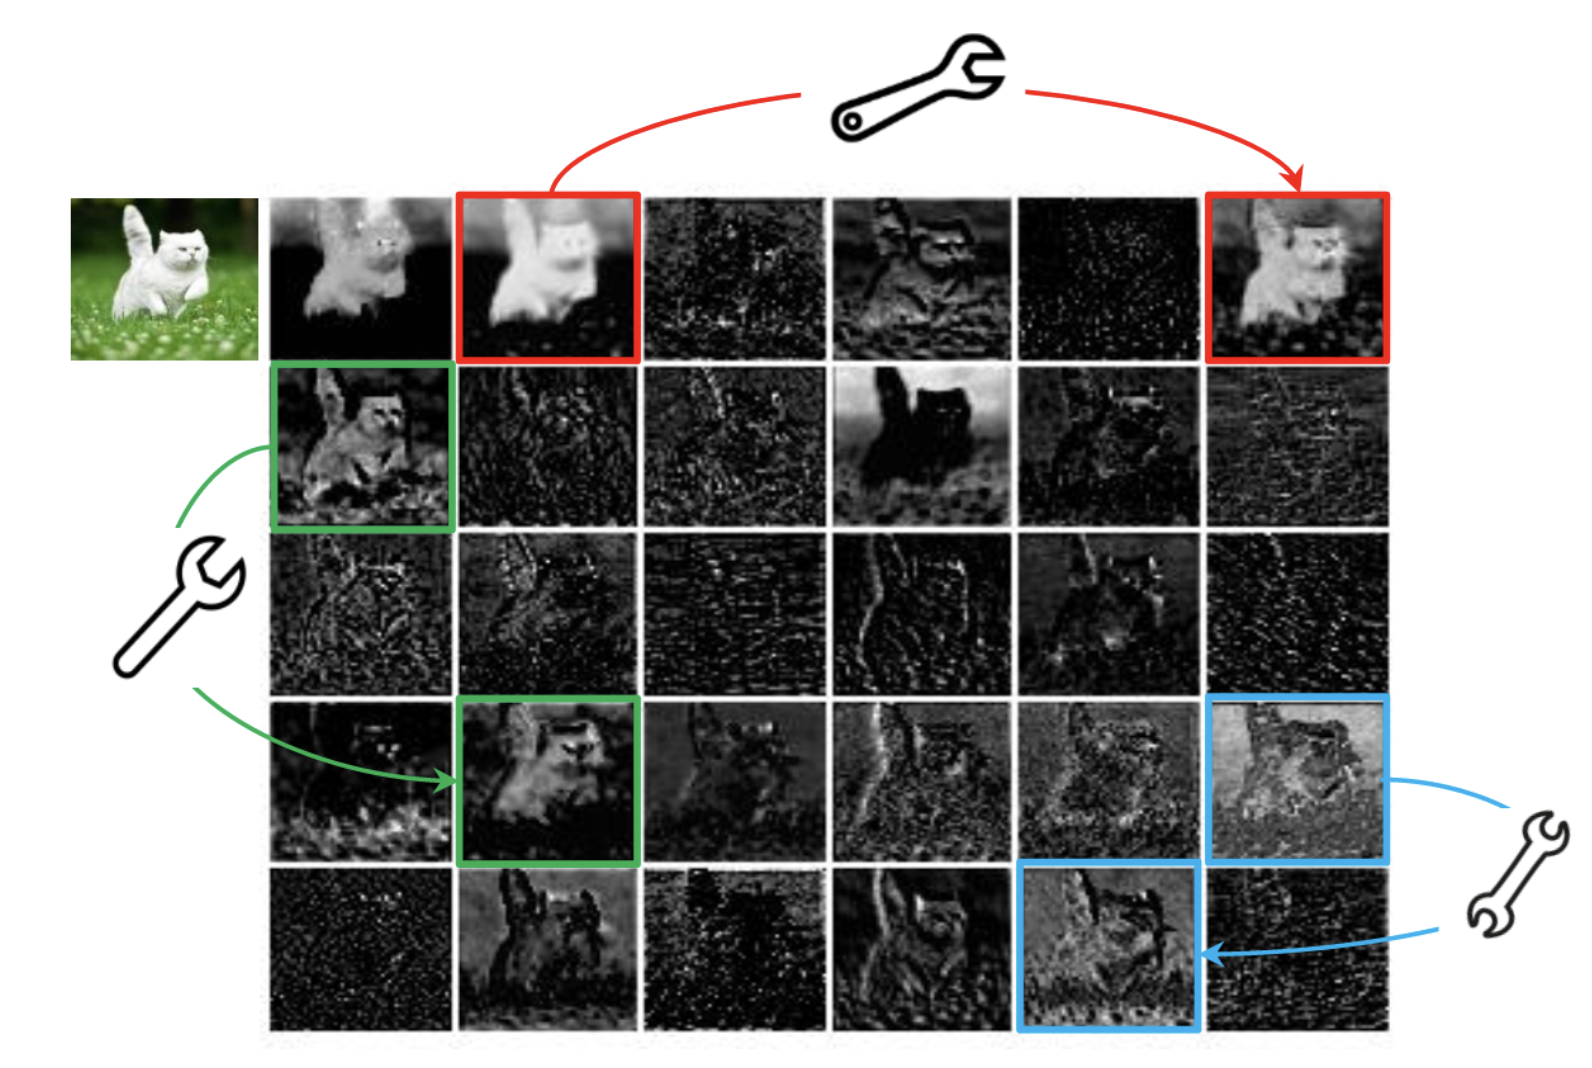
\includegraphics[width=0.8\textwidth]{thesis-template-master/images/ghostpointwise.png}
\label{fig:cellnet}
\end{center}
\caption{\textbf{Visualization of some feature maps generated by the first residual group in ResNet-50 \cite{19}}.  Three similar feature map pair examples are annotated with boxes of the same color. One feature map in the pair can be approximately obtained by transforming the other one through cheap operations (denoted by spanners). Point-wise convolution can extract more high-level features such as edge, shape, color, but a large amount of point-wise convolution results in massive computational costs  and generated much redundant map.}
\label{fig:2.7}
\end{figure}


\subsection{ More Features from Cheap Operation}


\begin{figure}[t]
\begin{center}
\centering
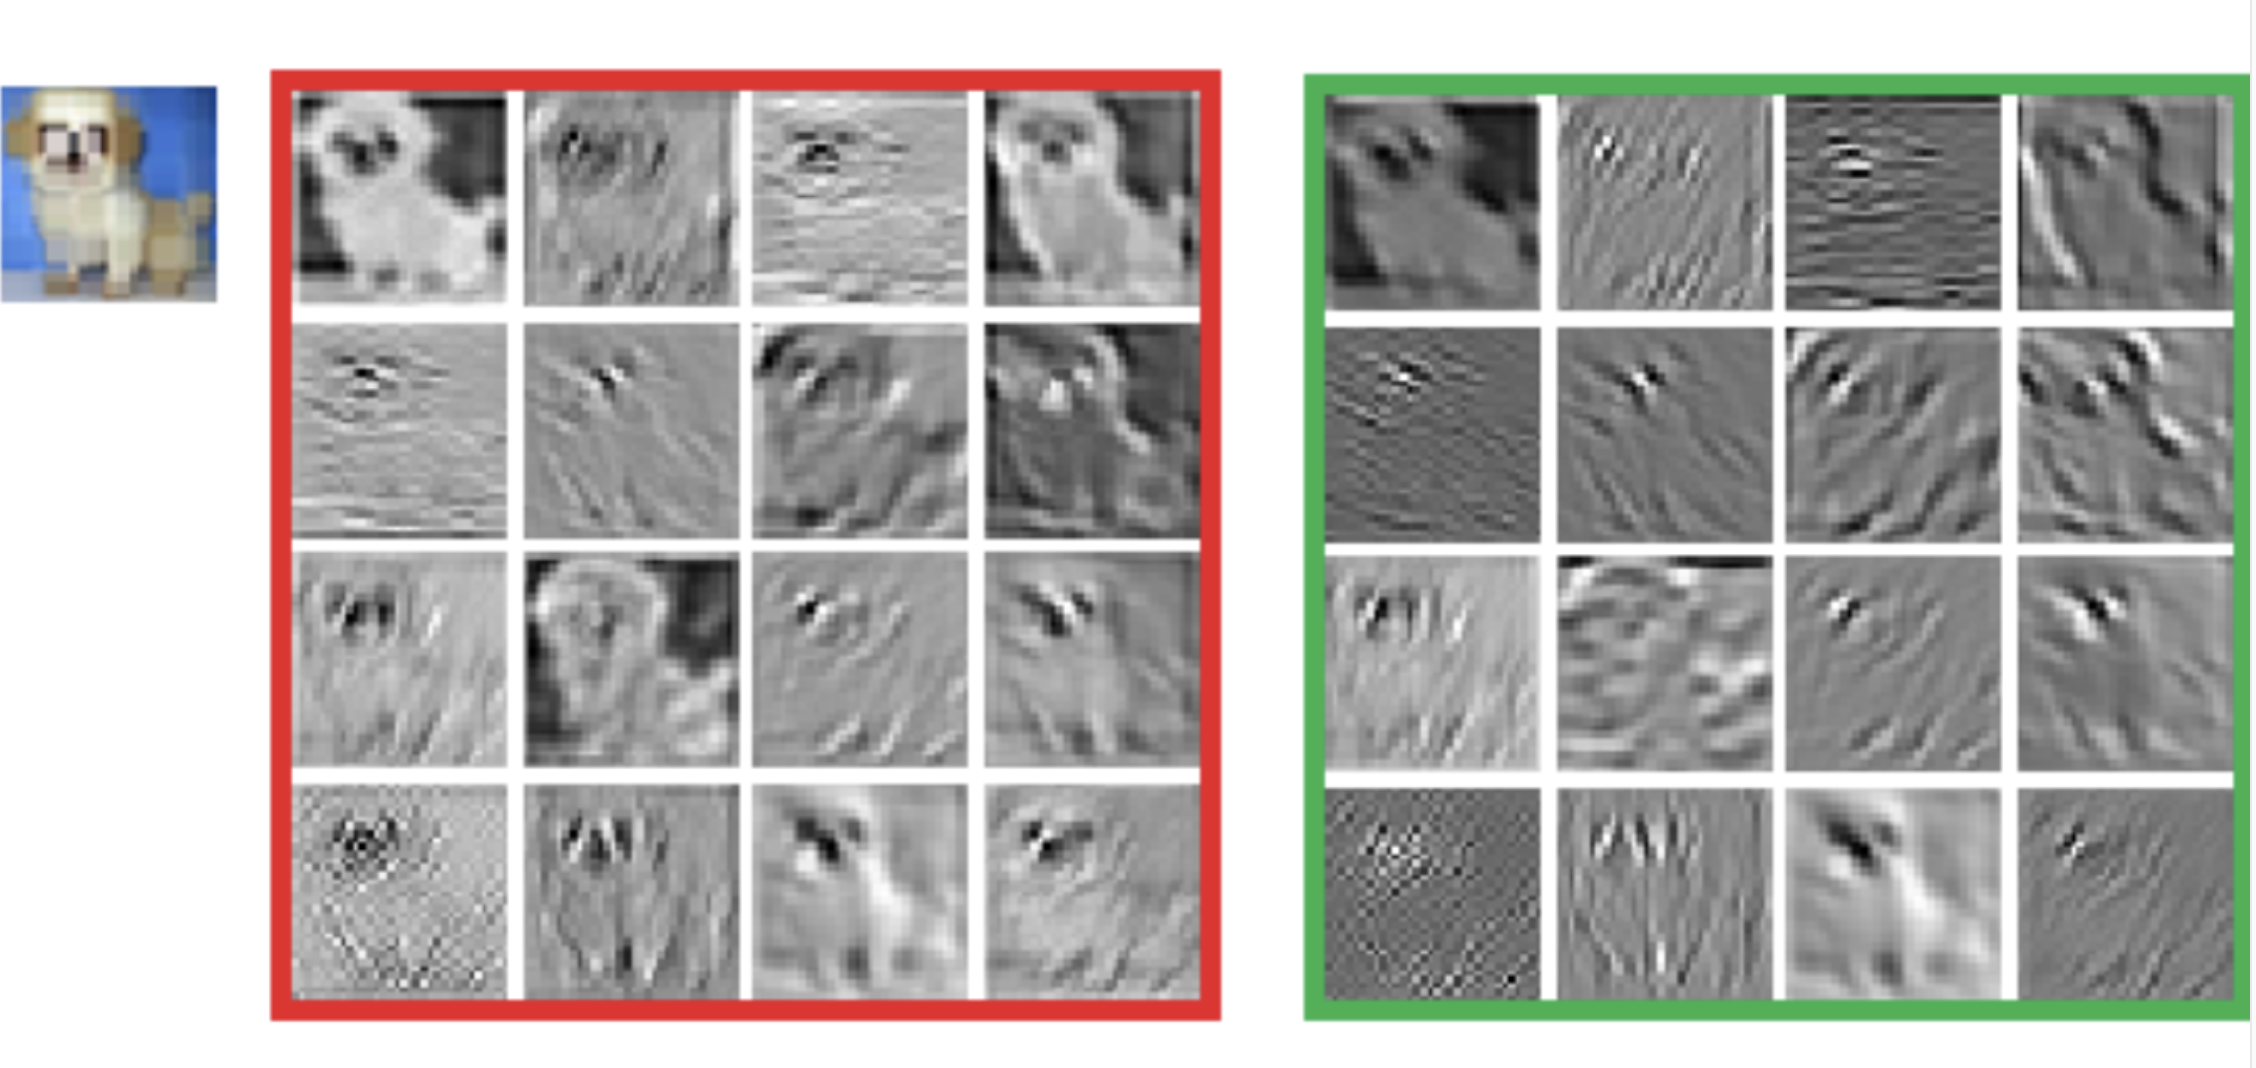
\includegraphics[width=\textwidth]{thesis-template-master/images/ghostgener.png}
\label{fig:cellnet}
\end{center}
\caption{\textbf{The feature maps in the 2nd layer of Ghost-VGG-16  \cite{19}}.  The left-top image is the input, the feature maps in the left red box are from the primary convolution, and the feature maps in the right green box are after the depthwise transformation.}
\label{fig:2.8}
\end{figure}

MobileNet \cite{30} and ShuffleNet \cite{29} have introduced depthwise convolution or shuffle operation to build efficient CNNs using  smaller convolution  filters  (floating-number operations).

Ghost net\cite{19} supposed that the output feature maps are "ghosts" of a handful of intrinsic feature maps with some cheap transformations, and these intrinsic feature maps are often of smaller size and produced by ordinary convolution filters. Using a primary convolution to generate those intrinsic feature maps and then applying a series of cheap linear operations on each intrinsic feature a  set of ghost features. It is worthy to note that those actions cost less computation power and in need of fewer weights. In practice, there could be several different linear operations in a Ghost module, such as customized size linear kernels depth-wise convolution, or linear transformations\cite{19}.

The limitation of the original GhostNet \cite{19} is that it still keeps numerous layers and does not get rid of convolutional manipulation. Moreover, it did not provide further experiments on how well the Ghost module can be generalized and integrated into other leading neural networks. These will be investigated in our thesis design.















\chapter{Methodology}
\label{sec:Methodology}
The purpose of this thesis is to invent a unifying approach capable of imaging single-cell morphology of thousands of peripheral blood cells and data-driven learning of characteristic mythologies indicative of the presence of the disease. With this in mind, we introduce a novel family of deep hierarchical network architectures called AttentionNet. Its goal is to land a well-established but straightforward network architecture for nearly-semantic segmentation to ensure higher precision classification tasks. Thus, we can base our claims about the multi-Scale prediction framework and multiple layers concatenation of original YOLOv3 \cite{33} architecture on a variety of experiments  (see Chapter 5). AttentionNet aims to combine lighter-weight layers and K Means++ techniques in pre-processing, and GBCIOU multi-object segment techniques to achieve the nearly-semantic segmentation for cells with lower computation cost and complexity.

For biomedical image processing, due to different experimental conditions, such as lighting conditions and various empirical objects, noise deviations are likely to appear on the sampled cell images\cite{6}\cite{7}, that noise and variability in the background would be confounding variables.
When applying AttentionNet, we explicitly learn features focusing on the morphology structure of the cell, as we mainly design the unifying approach for Sezary cell diagnosis, an aggressive cutaneous T cell lymphoma characterized by tumor T cells with abnormal nucleus morphology in the peripheral blood\cite{6}\cite{7}. Hence, we assume that after AttentionNet segmentation, convolutions are more likely to learn feature representations particularly for cell objects, as only the cell objects are preserved.

Modern architectures leverage multi-scale hierarchies to learn feature representations at different resolutions,i.e., from fine-grained and highly localized features to coarse but semantically enriched features, such as original YOLO network\cite{yolov1} and other state-of-the-art models. On the other hand, it also raises the network's complexity, requires high computational cost, and has insufficient sensitivity to customer datasets.

AttentionNet discards the Darknet\cite{33} part of original YOLO\cite{yolov1}, i.e., a multi convolutional stacked layer, and relies on only two YOLO output layers. Because the prior predicted box is known upfront by k-Mean++ clustering, only a few up-sampling layers additional are needed to give a satisfying accurate prediction of the cell position. Then, the circle detection algorithm will convert the bounding box to nearly semantic cell prediction while guaranteeing user-defined character requirements of the cell structure.

NMS(Non-Maximum Suppression) of YOLOv3\cite{33} will only remove highly overlapping prediction boxes that occupy a lower class score. YOLOv3\cite{33}  cannot guarantee excellent performance in cases such as multiple cells have high objectiveness scores and overlap with each other, or multiple cells do not overlap but do present in the same frame. Therefore, it is inevitable to utilize our GBCIOU algorithm to eliminate objects with relatively lower objectiveness scores while maximizing the retention of overlapping.

It is worth noting that the AttentionNet is not involved in the task of cell classification. Therefore, we purpose the Cellnet for cell classification.  The main novelty of CellNet is that it creatively combines the features of ResNet\cite{20} that are easy to expand, easy to understand, and extremely high classification accuracy, and the functionality of GhostNet\cite{19} module that uses a small amount of cheap linear operation to reduce redundant feature maps. Here, we introduce our new ghost module by adding the SE layer\cite{24} to better scaling less distinct feature maps generated by the cheap linear operation. What is more, the modern architecture of eight ghost modules. It was thereby achieving a lighter weight, real-time processing, and higher classification accuracy network, especially suitable for complex medical data sets.



\section{AttentionNet}
\label{sec:lorem}


\subsection{Network Architecture} % (fold)
\label{sub:citations}

In Table 3.1, we present our multi-scale AttentionNet architecture, which adopts the YOLOv3-Tiny\cite{18} architecture as its fundamental building block to process more efficiently on small targets. We follow the same
symmetrical encoder-decoder architecture \cite{17} with additional skip-connections interconnected in the same hierarchy level. At each hierarchy level, we consecutively perform several point-wise convolutions. 

\begin{table}[h]
\centering

\scalebox{0.90}{
\begin{tabular}{@{}clllll@{}}
\toprule
\multicolumn{1}{l}{\textbf{layer}} & \textbf{Type}                & \multicolumn{1}{l}{\textbf{Filters}} & \textbf{Size/Stride} & \textbf{Input}       & \textbf{Output}                          \\ \midrule
0                                  & Convolutional                & 16                                   & $3\times3$/1       & 416\times416\times3            & 416\times416\times16                               \\
1                                  & Maxpool                      &                                      & $2\times2$/2                & 416\times416\times16           & 208\times208\times16                               \\
2                                  & Convolutional                & 32                                   & $3\times3$/1                & 208\times208\times16           & 208\times208\times32                               \\
3                                  & Maxpool                      &                                      & $2\times2$/2                & 208\times208\times32           & 104\times104\times32                               \\
4                                  & Convolutional                & 64                                   & $3\times3$/1                & 104\times104\times32           & 104\times104\times64                               \\
5                                  & Maxpool                      &                                      & $2\times2$/2                & 104\times104\times64           & 52\times52\times64                                 \\
6                                  & Convolutional                & 128                                  & $3\times3$/1                & 52\times52\times64             & 52\times52\times128                                \\
7                                  & Maxpool                      &                                      & $2\times2$/2                & 52\times52\times128            & 26\times26\times128                                \\
8                                  & Convolutional                & 256                                  & $3\times3$/1                & 26\times26\times128            & 26\times26\times256                                \\
9                                  & Maxpool                      &                                      & $2\times2$/2                & 26\times26\times256            & 13\times13\times256                                \\
10                                 & Convolutional                & 512                                  & $3\times3$/1                & 13\times13\times256            & 13\times13\times512                                \\
11                                 & Maxpool                      &                                      & $2\times2$/1                & 13\times13\times512            & 13\times13\times512                                \\
12                                 & Convolutional                & 1024                                 & $3\times3$/1                & 13\times13\times512            & 13\times13\times1024                               \\
13                                 & Convolutional                & 256                                  & $1\times1$/1                & 13\times13\times1024           & 13\times13\times256                                \\
14                                 & Convolutional                & 512                                  & $3\times3$/1                & 13\times13\times256            & 13\times13\times512                                \\
15                                 & Convolutional                & {\color[HTML]{CB0000} \textbf{18}}   & $1\times1$/1                & 13\times13\times512            & {\color[HTML]{CB0000} \textbf{$13\times13\times18$}} \\
16                                 & YOLO                         &                                      &                      &                      &                                          \\
17                                 & \textbf{Rout13}              &                                      &                      &                      &                                          \\
18                                 & Convolutional                & 128                                  & $1\times1$/1                & 13\times13\times256            & 13\times13\times128                                \\
19                                 & Upsampling                   &                                      & $2\times2$/2                & 13\times13\times256            & 26\times26\times128                                \\
20                                 & \textbf{Route 19, 8}         &                                      &                      &                      &                                          \\
21                                 & Convolutional                & 256                                  & $3\times3$/1                & 26\times26\times384            & 26\times26\times256                                \\
22                                 & Convolutional                & {\color[HTML]{CB0000} \textbf{18}}   & $1\times1$/1                & 26\times26\times256            & {\color[HTML]{CB0000} \textbf{$26\times26\times18$}} \\
23                                 & YOLO                         &                                      &                      &                      &                                          \\ \bottomrule

\end{tabular}}
\caption{\textbf{AttentionNet network structure}. Final YOLO Output should equal to $3\times(classes+5)$}
\end{table}

The attributes of self-detection and labeling, of nearly real-time resolve and general resource requirements mainly characterize the AttentionNet. In the beginning, it is similar to YOLOv3\cite{33} that the input image is divided into an $M \times M$ grid. Then $B$ bounding boxes and confidence scores are defined in each grid cell. Each grid cell predicts $C$ conditional probabilities, denoted as $P(Class_{i}\mid Object_{j})$ for $i$ classes and object $j$. If there is an object $j$ in the grid, then indicated the objectiveness score $P(Object_{j})$  equal to $1$\cite{18}. Here, we refer to the initiatives from YOLOv3\cite{33}, and the confidence score also represents the confidence of the box prediction, define as $GIOU_{Ground truth}^{Predition}$. Unlike the originally YOLOv3\cite{33}, instead of using Intersection‐Over‐Union (IOU), we use $GIOU$ with higher precision, which refers to the generalized intersection area between the predicted bounding box and ground truth box.

It should be noted that each grid cell predicted conditional class probability is not the same as the confidence score. These often leads to misunderstanding of the fact that the former $P(Class_{i} \mid Object_{j})$ is predicted in each grid, while the $P(Object_{j}) \times GIOU_{Ground truth}^{Predition}$ is predicted in each bounding box\cite{18}. 
Finally Class Score $S$ is defined as follow (1): \label{eq}

\begin{equation}
\begin{split}
$S&=P(Class_{i}\mid Object_{j}) \times P(Object_{j}) \times GIOU_{Ground truth}^{Predition} \\
$& = P(Class_{i}) \times GIOU_{Ground truth}^{Predition} $\label{eq}
\end{split}
\end{equation}

The Class Score $ S $ computed the probability of the object $j \in  i$ class appearing in the box and how well the bounding box fits each object $j$.



\subsection{Multi Scale Tensor Prediction Framework}
\label{sub:fixme}

The original YOLOv3\cite{33} used the Darknet front-end feature extraction module, but the detection performance on Sezary Syndrom dataset is unsatisfied. On the contrary, AttentionNet with only $13 \times 13$, $26 \times 26$ YOLO scale output tensors adopts multi-scale fusion, and K means++ clustering\cite{18} techniques, outperforms TF-Yolo\cite{18} and  YOLOv3 \cite{33}, which occupied  $13 \times 13$, $26 \times 26$, $52 \times 52$ YOLO scale output tensor. In order to train a suitable segment-or, it is recommended to choose corresponding scale tensors that refer to different data sets. 

We use a YOLOv3\cite{33} like architecture due to its modularisation capabilities. In the ablation study, we individually measure the impact of all architectural components. Here, we vary the tensor Multi-Scale Tensor, as well as the number of hierarchy levels used by the architecture. Moreover, we modify the number of point-wise convolution layers to measure the effect of each Yolo tensor output independently and in parallel. Hence, we make reasonable
claims about the combination of only $13 \times 13$, $26 \times 26$ YOLO scale output tensors.

\begin{figure}[h]
	\begin{center}
		\begin{subfigure}[b]{0.49\textwidth}
			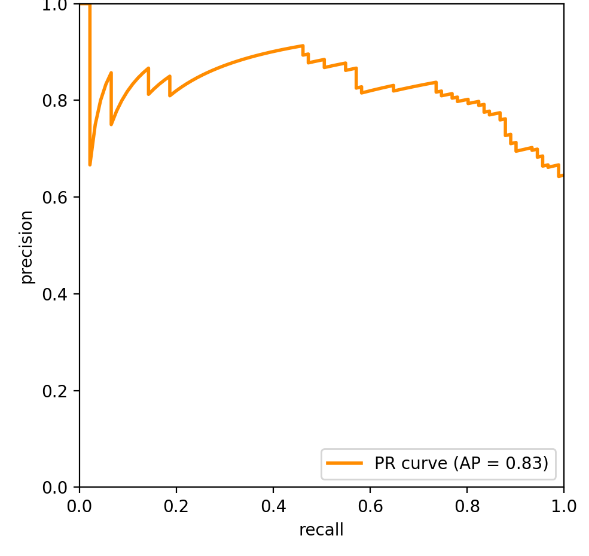
\includegraphics[width=\textwidth]{thesis-template-master/images/2 tensor cellyolo PR on val dataset.png}
			\caption{$13 \times 13$, $26 \times 26$ tensor }
			\label{fig:res18}
		\end{subfigure}
		\begin{subfigure}[b]{0.49\textwidth}
		    \centering
			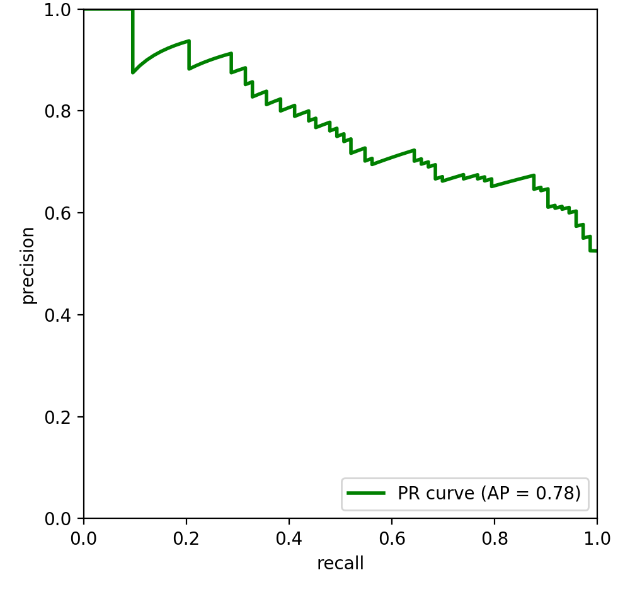
\includegraphics[width=\textwidth]{thesis-template-master/images/52 tensor cellyolo PR on val dataset.png}
			\caption{$52 \times 52$, $26 \times 26$tensor }
			\label{fig:cellnet}
		\end{subfigure}
	\end{center}
	\caption{\textbf{Precision-Recall curve on val dataset of Sezary Syndrom dataset in terms of different scale YOLO output layers.}. ,  Note: both measured on on val dataset: 1k training image, 726 test image.}
	\label{fig:3.1}
\end{figure}


\subsection{K‐means++ Clustering in Pre-processing}

K‐means++ clustering is an approach commonly used to adaptive partition a dataset into groups. It is necessary to specify the number of cluster centers in advance. The K‐means++ algorithm generally uses the Euclidean distance to measure the distance between two points. Instead of using the prior nine boxes given by YOLOv3\cite{33} trained on the COCO dataset, for our customer dataset, it is noteworthy that give the prior knowledge of the ground truth box. Utilizing a small subset of the manually annotated cell, we can improve $GIOU$(ground truth box position, prediction box location) scores. It will lead to better class scores and, in the final, achieve higher accuracy (see \eg\reffig{3.3}).


\begin{figure}[h]
	\begin{center}
		\begin{subfigure}[b]{0.49\textwidth}
			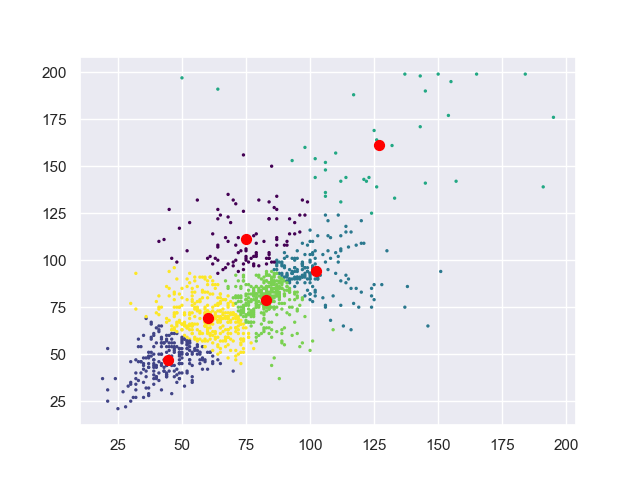
\includegraphics[width=\textwidth]{thesis-template-master/images/Figurefor 1480_1.png}
			\caption{ The cluster  distribution }
			\label{fig:res18}
		\end{subfigure}
		\begin{subfigure}[b]{0.49\textwidth}
		    \centering
			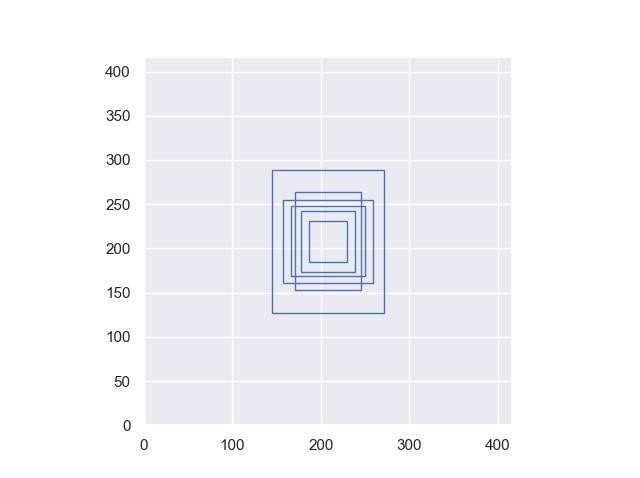
\includegraphics[width=\textwidth]{thesis-template-master/images/Figure_for1480.png}
			\caption{ Six prior boxs}
			\label{fig:cellnet}
		\end{subfigure}
		\begin{subfigure}[b]{0.49\textwidth}
			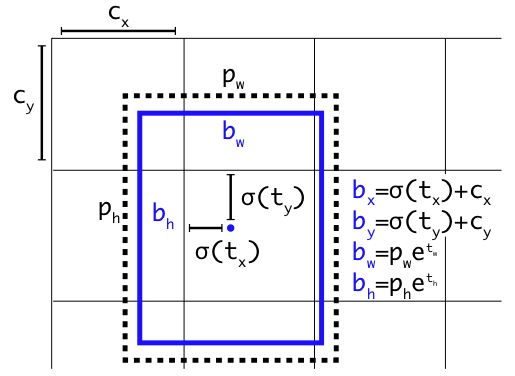
\includegraphics[width=\textwidth]{thesis-template-master/images/anchor.JPG}
			\caption{ Prior box and prediction box in YOLOv3\cite{33}}
			
		\end{subfigure}
	\end{center}
	\caption{\textbf{The illustrations of K-means++ applied in prior box acknowledgment}. (a) the dot represents the ground truth box$(w,h)$ ;(b) the six prior boxes clustered by K-Means++,  input by manually labeled ground truth boxes;(c)  the blue dotted line box represents the prediction box, and the smaller solid line box stands for bounding box predicted by grid cell.  Ground truth box as anchor box input could give the network the firsthand knowledge of cell size to help more accurate prediction.}
	\label{fig:3.2}
\end{figure}

The main steps of the K‐means++ method are as follows in Algorithm 1.
\begin{figure}[h]
	\begin{center}
		\begin{subfigure}[b]{0.49\textwidth}
		    \centering
			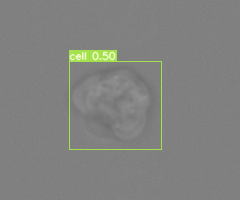
\includegraphics[width=0.9\textwidth]{thesis-template-master/images/withkmean.png}
			\caption{With K-means++ cluster}
			\label{fig:cellnet}
		\end{subfigure}
		\begin{subfigure}[b]{0.49\textwidth}
		    \centering
			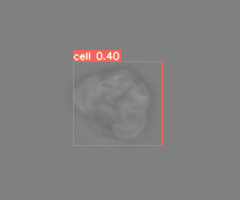
\includegraphics[width=0.9\textwidth]{thesis-template-master/images/withoutkmean.png}
			\caption{Without K-means++ cluster}
			\label{fig:cellnet}
		\end{subfigure}
		\begin{subfigure}[b]{0.49\textwidth}
		    \centering
			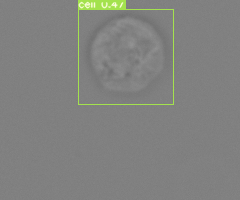
\includegraphics[width=0.9\textwidth]{thesis-template-master/images/withkmean1.png}
			\caption{With K-means++ cluster}
			\label{fig:cellnet}
		\end{subfigure}
		\begin{subfigure}[b]{0.49\textwidth}
		    \centering
			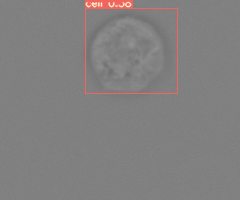
\includegraphics[width=0.9\textwidth]{thesis-template-master/images/withoutkmean2.png}
			\caption{Without K-means++ cluster}
			\label{fig:cellnet}
		\end{subfigure}
	\end{center}
	\caption{\textbf{The comparison on cell segmentation  performance between With / Without K-means++ cluster}. As (a) and (b) show clearly, the K-means++ cluster helps not only the score of the cell  and the degree of polymerization. }
	\label{fig:3.3}
\end{figure}


\begin{algorithm}[h]
  \caption{K‐means++ Clustering in ground truth boxes.}
  \label{alg:Framwork}
  \begin{algorithmic}[1]
    \Require
    manually labelled a series of ground truth $B^{i}$ bounding boxes coordinates:
     $B^{i}=\left ( x_{1}^{i},y_{1}^{i},x_{2}^{i},y_{2}^{i} \right ), i\in n.$ And clusters number $K$.
    \Ensure
    optimal  prediction box size $\left ( w,h \right )$
    \State For each box $B^{i}$, calculated the width and height by:
    
    $w^{i}=(x_{2}^{i}-x_{1}^{i}), h^{i}=(x_{2}^{i}-x_{1}^{i})$.
    
    \State Choose an initial center $t_{1}$ uniformly at random from the dataset $X=(w^{i},h^{i}),i\in n$.
    \While{$d\left ( x \right )$ shortest distance and  $K$ cluster not reached}
       \State Choose the next center $t_{i}$ , selecting $t_{i}={x}'\in X $ with probability $\frac{d ( {x}')^{2}}{\sum_{x\in X}^{}d\left ( x \right )^{2} }$
where $d\left ( x \right )$ is the distance from a data point $x$ to the closest cluster center.
       \State For $i \in \left \{ 1,2,...K \right \}$ , set the cluster $T_{i}$ to be the set of points in $X$ that are closer to
$t_{i}$ than they are to $t_{j}$ for all $i\neq j$.
    
  
    \Return $T_{i}=(w^{i},h^{i}),i \in K$.
  \end{algorithmic}
\end{algorithm}

As mentioned above, the YOLOv3\cite{33} algorithm has achieved end‐to‐end training and high‐speed target detection. However, some problems still exist: conventional YOLO \cite{yolov1} divides each image into a fixed grid, which results in a limited number of detected objects;  the fixed parameters provided by anchor are suitable for the targets in the VOC datasets, while they are not adapted to the targets in specific scenes. Common targets, such as vehicles, tanks, and airplanes, have a large aspect ratio. Therefore, this section takes advantage of the ideas in K-Means++ clustering. In the beginning,  we manually set a series of prior boxes for the network, select appropriate anchor box size, and adjust the network needs accordingly to real application domains. In this way, the AttentionNet network achieves nearly semantic prediction. Meanwhile, it is insensitive to small objects, particularly cell object.



\subsection{Loss function} % (fold)
\label{sub:citations}

Contrarily to the original implementation of YOLOv3\cite{33}, we calculate the loss function employing three parts. Here, we divide them into three compositions, the loss between the ground truth box and the prediction box, the confidence score loss, the final cross-entropy loss for the class label. The first part is the prediction bounding box loss; the second part indicates the confidence loss, and the final part represents the class label loss. in Equation (3.2), $k$ means the classes, the $conf$ states the confidence, and the 10,647 generated from 2,535 prediction bounding boxes. It is equal to $(13\times13\time3+26\time26\time3)=2,535$ in contrast to originally YOLOv3\cite{33} has $(13\times13\time3+26\time26\time3+26\time26\time3)=10,647$ prediction bounding boxes.

\begin{equation}
\begin{split}
$Loss&=\frac{1}{2}\sum_{i=1}^{2535}\lambda _{obj}\times \{ \left ( 2-truth_{w} \times truth_{h}\right )\times  \sum_{r\in \left ( x,y,w,h \right )}^{}\left ( truth_{r}-predict_{r} \right )^{2} \\$
$&+ \sum_{k-1}^{r=0} \left ( \left ( r==truth_{class} \right )-predict_{class_{r}} \right )^{2}  \} + \left ( truth _{conf}-predict_{conf}\right )^{2}$\label{eq}
\end{split}
\end{equation}

\textbf{ The Loss for Bounding Box}:
\begin{equation}
\begin{split}
$\lambda _{obj}\times \left  \left ( 2-truth_{w} \times truth_{h}\right )\times \sum_{r\in \left ( x,y,w,h \right )}^{}\left ( truth_{r}-predict_{r} \right )^{2}$ \label{eq}
\end{split}
\end{equation}
In YOLO\cite{yolov1}, the author did find the square root of the width and height (w, h) to weakening the influence of the bounding box size on the loss value. Here, we are following YOLOv3\cite{33} priority suggestions do not adopt the square root method, but added a weight-related to the quantity of the object box size, namely with weight = $  2-truth_{w} \times truth_{h}  $, value range from $(1~2)$. In contrast to the first version of the YOLO network, which adopted the IOU loss to calculate the loss between prediction box and prior, the YOLOv3\cite{33} improved the accuracy by 1\% under the contribution of GIOU loss. 

\begin{algorithm}[htb]
  \caption{ Generalized Intersection over Union(GIoU) as Bounding Box loss.}
  \label{alg:Framwork}
  \begin{algorithmic}[1]
    \Require
    Predicted $B^{p}$ and ground truth $B^{g}$ bounding box coordinates:
     $ B^{p}=\left ( x_{1}^{p},y_{1}^{p},x_{2}^{p},y_{2}^{p} \right ),B^{g}=\left ( x_{1}^{g},y_{1}^{g},x_{2}^{g},y_{2}^{g} \right ).$
    \Ensure
     GIoU loss $L_{GIoU}$;
    \State For the predicted box $B^{p}$, ensuring $x_{2}^{p} > x_{1}^{p}$ and $y_{2}^{p} > y_{1}^{p}$:
    
    $\hat{x}_{1}^{p}=min( x_{1}^{p},x_{2}^{p})$, $\hat{y}_{1}^{p}=min( y_{1}^{p},y_{2}^{p})$,
    $\hat{x}_{2}^{p}=max( x_{1}^{p},x_{2}^{p})$, $\hat{y}_{2}^{p}=max( y_{1}^{p},y_{2}^{p})$.

    
    \State Calculating the area of $B^{g}$:
    $A^{g}=(x_{2}^{g}-x_{1}^{g}) \times (y_{2}^{g}-y_{1}^{g})$
   
    \State  Calculating the area of $B^{p}$:
    $A^{p}=(\hat{x}_{2}^{p}-\hat{x}_{1}^{g}) \times (\hat{y}_{2}^{p}-\hat{y}_{1}^{p})$
    
    \State Calculating the intersection area $I$ between  $B^{g}$and  $B^{p}$:
    
    $x_{1}^{I}=max( \hat{x}_{1}^{p},x_{1}^{g})$, $y_{1}^{p}=max( \hat{y}_{1}^{p},y_{1}^{g})$,
    $x_{2}^{I}=min(\hat{x}_{2}^{p},x_{2}^{g})$, $y_{2}^{p}=min(\hat{y}_{2}^{p},y_{2}^{g})$.
    \If {$x_{1}^{I} < x_{2}^{I},  y_{1}^{I} < y_{2}^{I} $}
      \State  $I= (x_{2}^{I}-x_{1}^{I}) \times (y_{2}^{I}-y_{1}^{I})$ 
    \Else
      \State $I \gets 0$
      
    \EndIf
    \State Finding the coordinate of the smallest enclosing convex object $C$:
      $ C=\left ( min( \hat{x}_{1}^{p},x_{1}^{g}), max(\hat{x}_{2}^{p},x_{2}^{g}),
      min( \hat{y}_{1}^{p},y_{1}^{g}), max(\hat{y}_{2}^{p},y_{2}^{g}) \right )$
    
    \State Calculating area of the smallest enclosing convex object $S^{C}$
    \State $IoU=I/( A^{g} + A^{p} - I)$
    \State $GIoU=  IoU -\frac{S^{C}-A^{g} - A^{p} + I}{S^{C}}$
    \State $L_{GIoU}=1-GIoU$
    \newline
    \Return $L_{GIoU}$.
  \end{algorithmic}
\end{algorithm}

The bounding box is generally composed of the upper left and lower right corners of the coordinates, denoted as ($x_{1}, y_{1}, x_{2}, y_{2}$). Note that this is actually a vector, and vector distances are generally can be measured by either the $ L_{1}$ norm or the $ L_{2}$ norm. However, it was found that the values of both IOU and GIOU are very different, indicating that the use of the $L$ paradigm to measure the distance between the prediction and the real ground truth is inappropriate, as shown in  \eg\reffig{3.4}.



\begin{figure}[h]
	\begin{center}
		\begin{subfigure}[b]{0.49\textwidth}
		    \centering
			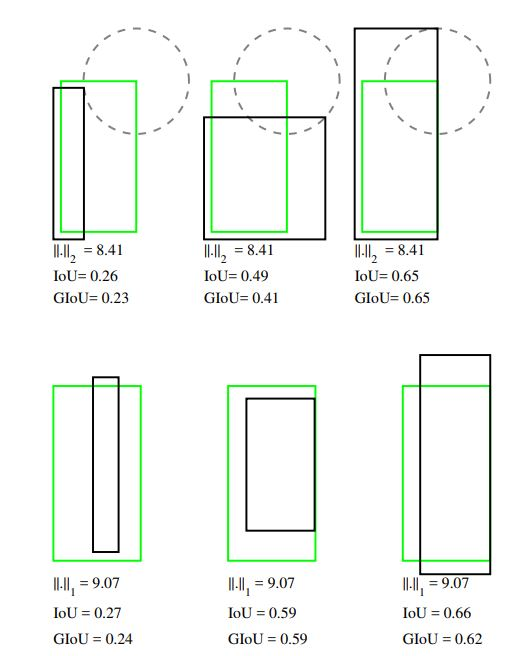
\includegraphics[width=\textwidth]{thesis-template-master/images/l2loss.JPG}
			\label{fig:cellnet}
		\end{subfigure}
	\end{center}
	\caption{\textbf{Two sets of examples with the bounding box}.
boxes represented by two corners  ($x_{1}, y_{1}, x_{2}, y_{2}$)  for first row, center and size  ($x_{c}, y_{c}, w, h$). for second row. For all three cases in each set  $ L_{1}$ norm distance, and the $ L_{2}$ norm distance, between the representation of two rectangles are exactly same value, but their IOU and GIOU values are very different.}
    \label{fig:3.4}
\end{figure}

The IOU is commonly used in academia to measure the similarity between two boundaries, but we found that there are two obvious drawbacks to using IOU, making it less suitable for the loss function.

First, when there is no overlap between the prediction box and the ground truth. An IOU value of 0 results in a gradient of 0 when optimizing the loss function, meaning that optimization is impossible.

Secondly, even if the prediction box and the real box overlap and have the same IOU value, the detection effect will differ. It is indistinguishable by IOU because IOU is the same, but GIOU various. If the two bounding boxes overlap, the better the alignment, the higher the GIOU value.

\textbf{ The confidence score loss}:
\begin{equation}
\begin{split}
$\left ( truth _{conf}-predict_{conf}\right )^{2}$ \label{eq}
\end{split}
\caption{\textbf{The Loss for Bounding Box}.}
\end{equation}

Here, we should find the prediction bounding box with the most massive IOU value of the real ground truth. If the most massive IOU is less than the threshold, then the prediction contains no objects, and it is the background grid. Then we calculate the confidence loss (we hope that if the grid contains objects, then the confidence of the prediction box output is 1, and 0 when there is no object). The confidence $\lambda _{obj}$ comes from focal loss. It indicates the confidence level to determine if there is an object in the grid.

\textbf{ The cross entropy loss for class label:}
\begin{equation}
\begin{split}
$\lambda _{obj}\times \sum_{k-1}^{r=0}  ( ( r==truth_{class}  )-predict_{class_{r}} )^{2} $ \label{eq}
\end{split}
\caption{\textbf{The Loss for Bounding Box}.}
\end{equation}
Finally, we utilize the cross-entropy loss to generate the class label.


\subsection{GBCIOU and Circle segmentation}
\label{sub:fixme}



\begin{algorithm}[htb]
  \caption{ GBCIOU for objects overlapping}
  \label{alg:Framwork}
  \begin{algorithmic}[1]
    \Require
     Two cell object Prediction $A$ and $B$ bounding box coordinates in the same flame:
     $ B=\left ( x_{1}^{b},y_{1}^{b},x_{2}^{b},y_{2}^{b} \right ),A=\left ( x_{1}^{a},y_{1}^{a},x_{2}^{a},y_{2}^{a} \right ).$ And confidence Score of each object $S^{b}>S^{a}$.
    \Ensure
     Optimal prediction box $P$. 
    \State For the box $A$ and $B$, ensuring: $x_{2}^{b} > x_{1}^{b}$, $y_{2}^{b} > y_{1}^{b}$, $x_{2}^{a} > x_{1}^{a}$, $y_{2}^{a} > y_{1}^{a}$.
    \State Calculate the intersection area:
    
    $I= (min(x_{2}^{a}, x_{2}^{b}) - max(x_{1}^{a}, x_{1}^{b})) \times (min(y_{2}^{a},y_{2}^{b})- max(y_{1}^{a},y_{1}^{b})) $
    \State Calculating the Union area, contrarily to the original Union we add small $1e-16 $
    to balance the integral side effect of $A$ and $B$ bounding box coordinates, but it will not effect the $GIoU$: 
    $Union= (x_{2}^{b}-x_{1}^{b}) \times (y_{2}^{b}-y_{1}^{b})+ 1e-16 + (x_{2}^{a}-x_{1}^{a}) \times (y_{2}^{a}-y_{1}^{a}) -I $
    \State Finding the coordinate of the smallest enclosing convex object $C_{w,h}$: 
    
    $ w, h= max(x_{2}^{a}, x_{2}^{b}) - max(x_{1}^{a}, x_{1}^{b}), max(y_{2}^{a},y_{2}^{b}) - max(y_{1}^{a}, y_{1}^{b})$
    \State Calculating  enclose area  $E$: $E = w \times h + 1e-16$
    \State Calculating  $GIoU$: $GIoU= \frac{E - Union}{E}$ 
    \If { $GIoU < threshold $}
      \State  $P \gets( min(x_{1}^{a}, x_{1}^{b}), min(y_{1}^{a},y_{1}^{b}),max(x_{2}^{a}, x_{2}^{b}),max(y_{2}^{a},y_{2}^{b})) $ 
    \Else
      \State $P \gets (x_{1}^{b},y_{1}^{b},x_{2}^{b},y_{2}^{b})$
    \EndIf
    
    \Return $P$
    
  \end{algorithmic}
\end{algorithm}




\begin{figure}[h]
	\begin{center}
		\begin{subfigure}[b]{0.25\textwidth}
		    \centering
			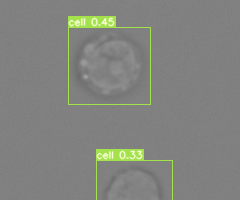
\includegraphics[width=\textwidth]{thesis-template-master/images/gbciou1.png}
			\caption{}
			\label{fig:cellnet}
		\end{subfigure}
		\begin{subfigure}[b]{0.25\textwidth}
		    \centering
			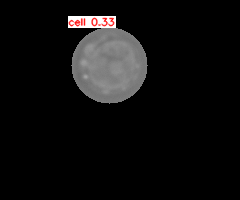
\includegraphics[width=\textwidth]{thesis-template-master/images/gbciou2.png}
			\caption{}
			\label{fig:cellnet}
		\end{subfigure}
		\begin{subfigure}[b]{0.25\textwidth}
		    \centering
			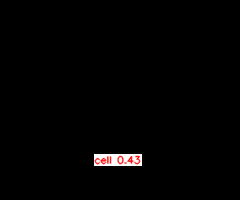
\includegraphics[width=\textwidth]{thesis-template-master/images/gbciou3.png}
			\caption{}
			\label{fig:cellnet}
		\end{subfigure}
		\begin{subfigure}[b]{0.25\textwidth}
		    \centering
			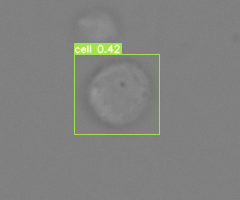
\includegraphics[width=\textwidth]{thesis-template-master/images/gbciou7.png}
			\caption{}
			\label{fig:cellnet}
		\end{subfigure}
		\begin{subfigure}[b]{0.25\textwidth}
		    \centering
			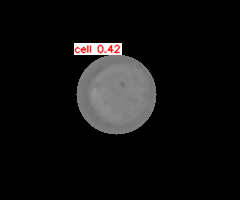
\includegraphics[width=\textwidth]{thesis-template-master/images/gbciou8.png}
			\caption{}
			\label{fig:cellnet}
		\end{subfigure}
		\begin{subfigure}[b]{0.25\textwidth}
		    \centering
			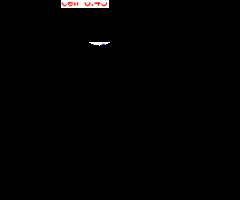
\includegraphics[width=\textwidth]{thesis-template-master/images/gbciou9.png}
			\caption{}
			\label{fig:cellnet}
		\end{subfigure}
		\begin{subfigure}[b]{0.25\textwidth}
		    \centering
			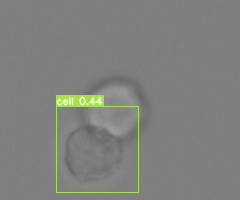
\includegraphics[width=\textwidth]{thesis-template-master/images/gbciou10.png}
			\caption{}
			\label{fig:cellnet}
		\end{subfigure}
		\begin{subfigure}[b]{0.25\textwidth}
		    \centering
			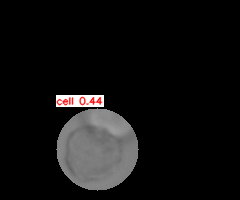
\includegraphics[width=\textwidth]{thesis-template-master/images/gbciou11.png}
			\caption{}
			\label{fig:cellnet}
		\end{subfigure}
		\begin{subfigure}[b]{0.25\textwidth}
		    \centering
			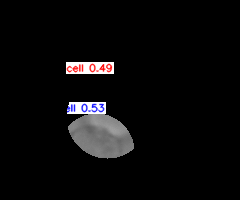
\includegraphics[width=\textwidth]{thesis-template-master/images/gbciou12.png}
			\caption{}
			\label{fig:cellnet}
		\end{subfigure}
	\end{center}
	\caption{\textbf{Experiments on GBCIOU for multiple predictions occur in same cell images.}(a),(d) and(g) stand for original cell bounding box detection, especially multiple cells overlapping or present in the same frame.(b),(e) and (h) represents with  GBCIOU circle segmentation, contrast to (c),(f) and(i) without GBCIOU. With help of GBCIOU, it obtains the best segmentation performance on cell.}
	\label{fig:3.5}
\end{figure}

Using the cvfillPoly function, we can easily classify the cell image into unaffected polygonal areas and achieve high-speed segmentation once we obtain the output from the AttentionNet network for bounding box detection, namely ($x_{1}$, $y_{1}$, $x_{2}$, $y_{2}$). However, it has undeniable shortcomings that the shape of the segmentation does not perfectly approximate the ground truth of the cell. To overcome this problem, we proposed a $ HSV $ space mask threshold method, It quietly converted to $ HSV $ space and used a threshold to eliminate the outside part of the central circle of box detection.  For the common challenge of the YOLO original version\cite{yolov1}: when multiple objects are standing in the same area or overlapping in the central point, it will become much more challenging to draw the correct prediction and always leads to wrong labeling. If multiple cells occur and one cell has a more competitive confidence score than another during circle detection, that will lead to either non-labeled or partly labeled problem.

We proposed the GBCIOU function to ideally find a general intersected box center when multiple box predictions occur in the same image, in addition to the GIOU (general interaction of union) computes the deviation between ground truth and the prediction.

\section{CellNet}
\label{sec:ipsum}


\subsection{Network Architecture} % (fold)
\label{sub:Network Architecture_2}
Inspired by those two outstanding neural network\cite{19}\cite{20}, instead of stacking lots of point-wise convolutional layers and taking a massive amount of convolutional manipulations, we can avoid the redundant feature maps by the cheap operation. 


As shown in Table 3.2, the first layer of CellNet is a standard convolutional layer with 64 filters, follows standard batch normalization and relu, generates initial intrinsic feature maps, then purpose a few series of G-bneck, in total eight layers. In each stage, we first apply stride = 1 then apply stride = 2 bottlenecks, which gradually increase the output channel dimension. After eight layers feature extraction, we get a 512-dimensional feature vector by global average pooling and convolutional layer. SE layer\cite{24} applied to scale less important feature map. Smoothing, blurring, and motion are also widely used in linear operation\cite{19}, but they need more GPU support. Utilizing a depth-wise convolution layer, we can generate more correlated ghost feature maps at a cheaper cost.

\begin{figure}[h]
	\begin{center}
		\begin{subfigure}[t]{0.49\textwidth}
		    \centering
			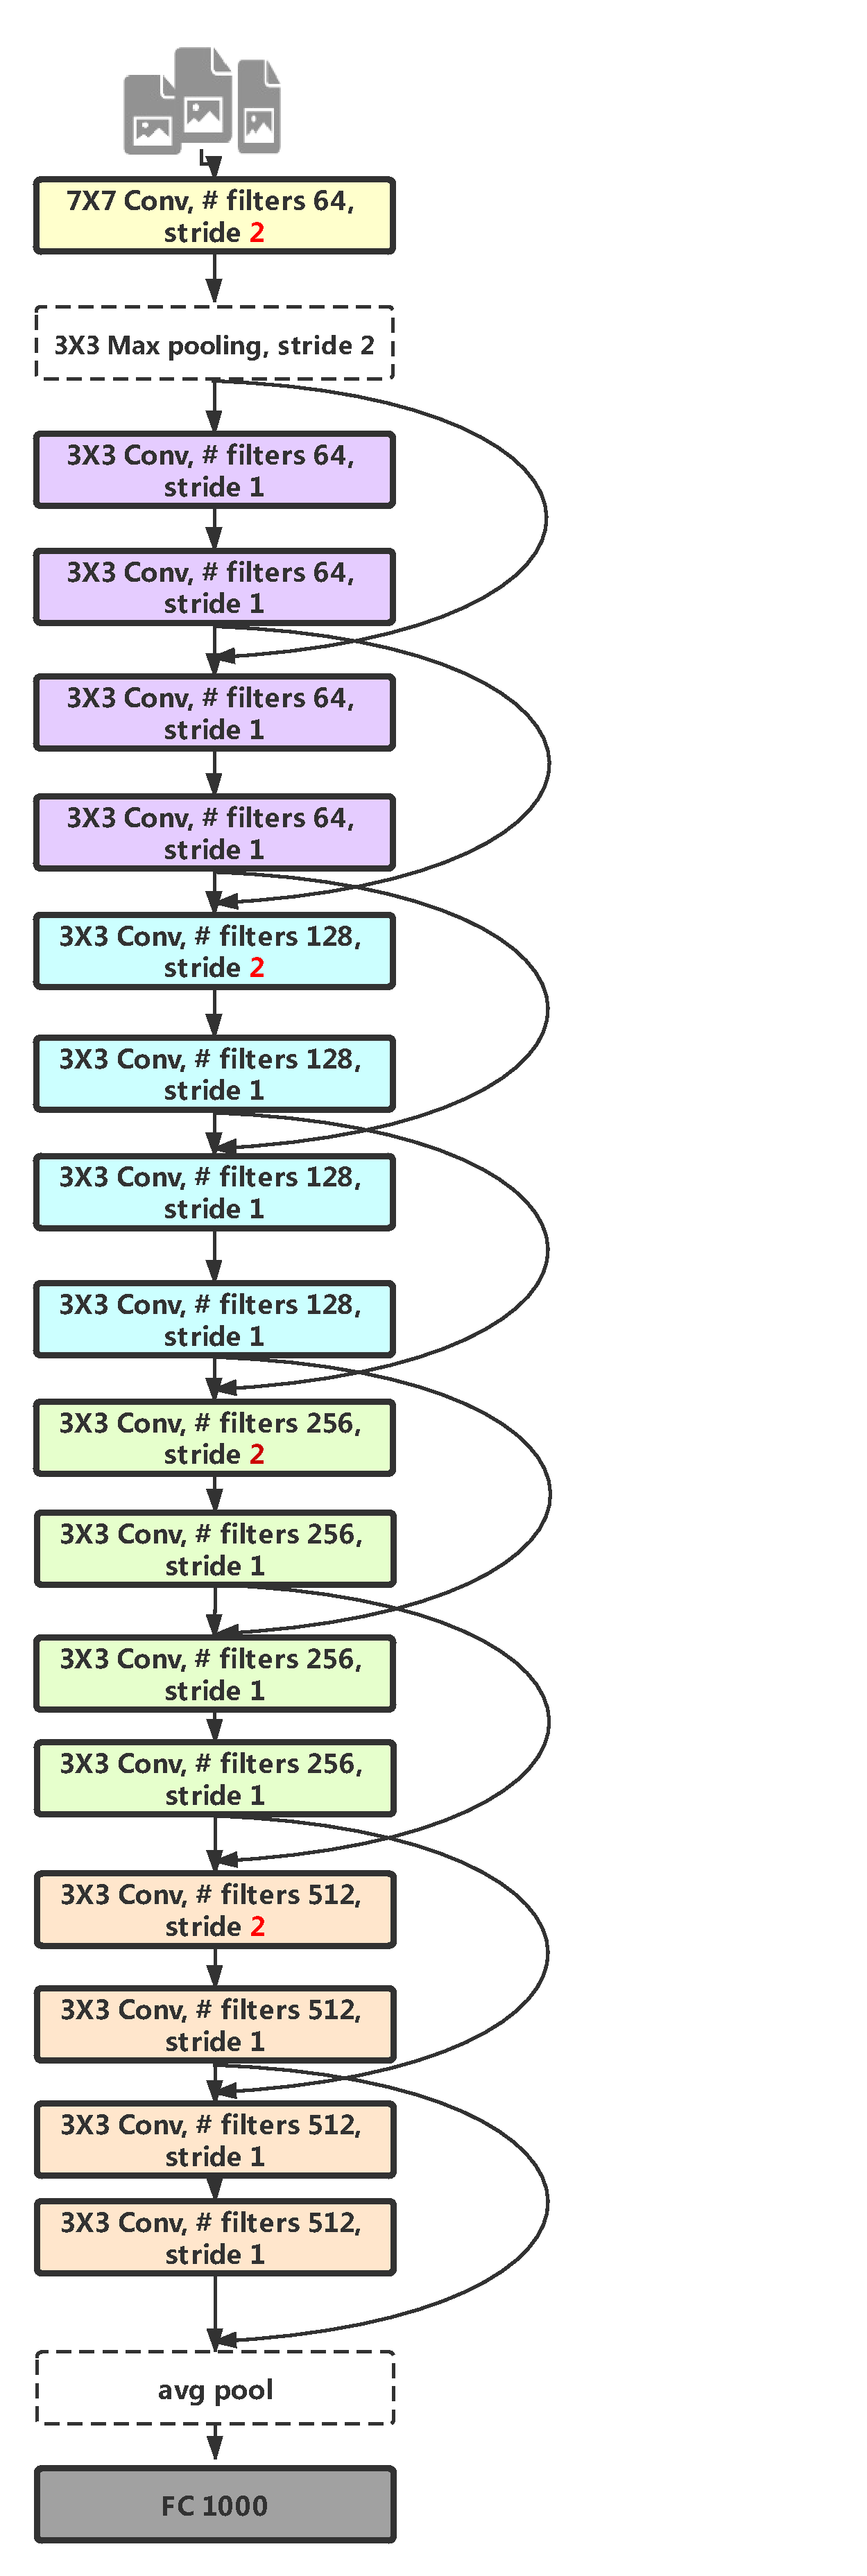
\includegraphics[height=6in]{thesis-template-master/images/res18.pdf}
			\caption{Overall architecture of ResNet18}
			\label{fig:res18}
		\end{subfigure}
		\begin{subfigure}[t]{0.49\textwidth}
		    \centering
			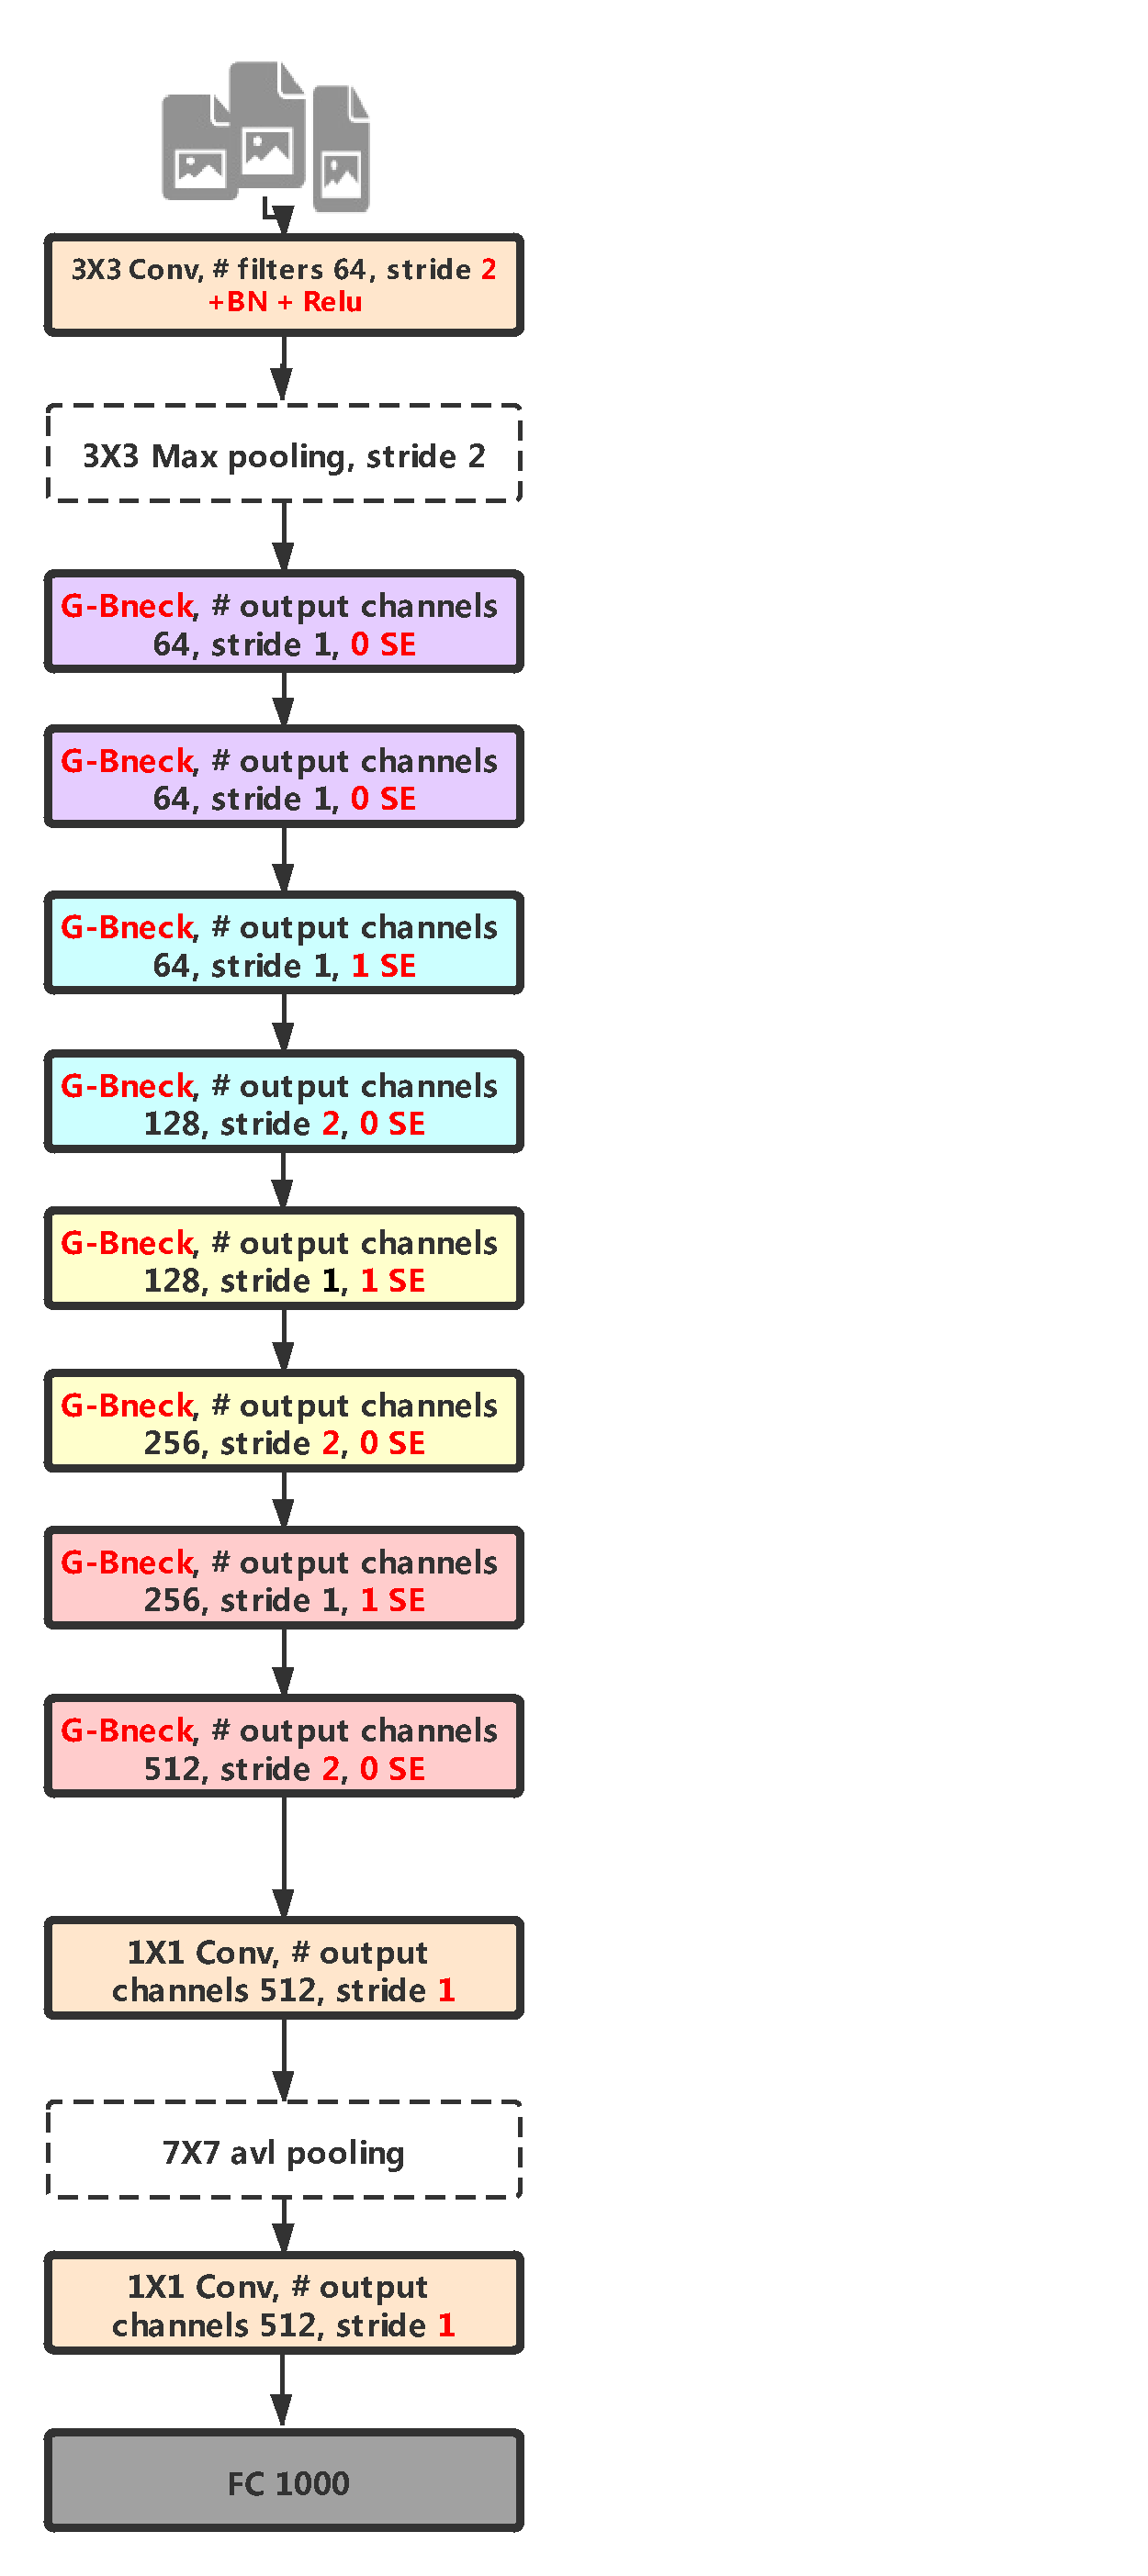
\includegraphics[height =5in]{thesis-template-master/images/Ghostres18.pdf}
			\caption{Overall architecture of CellNet}
			\label{fig:cellnet}
		\end{subfigure}
	\end{center}
	\caption{\textbf{The comparison between ResNet18 \cite{20} and CellNet}. Despite its simplicity (only eight layers ghost module) and lower parameters ( $1/4$ weights than ResNet18 \cite{20}), inside G-bottleneck adopted residual function for deeper gradient forward.}
	\label{fig:3.6}
\end{figure}








\subsection{Novel Ghostmodule} % (fold)
\label{sub:amet}

\begin{figure}[h]
	\begin{center}
		\begin{subfigure}[b]{\textwidth}
		    \centering
			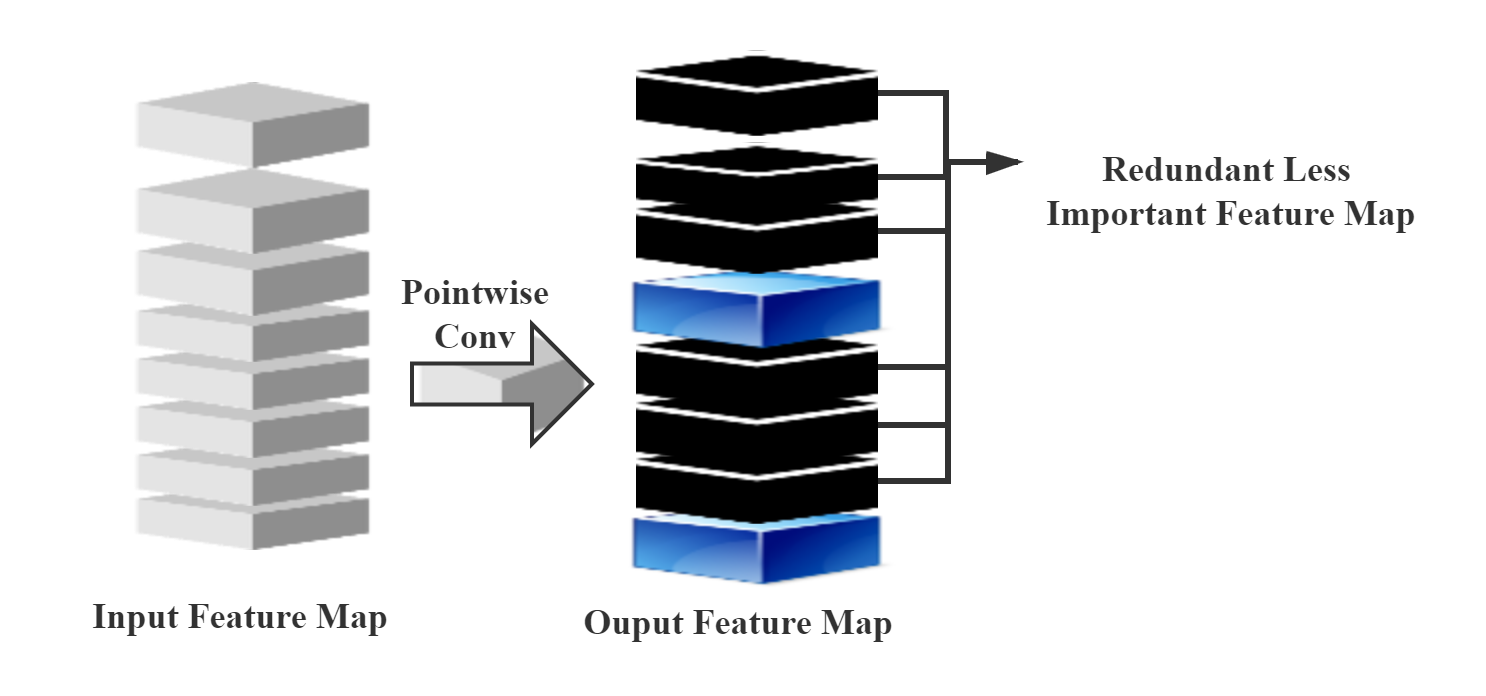
\includegraphics[width=\textwidth]{thesis-template-master/images/normal conv.png}
			
			\label{fig:cellnet}
		\end{subfigure}
	\end{center}
	\caption{\textbf{The normal Convolutional layer in \cite{26}\cite{27}\cite{28}}. As it illustrated that to extract the same amount of feature map, there are much more redundant output feature maps by taking point-wise convolution, especially for the small target objects or less informative images.}
	\label{fig:3.7}
\end{figure}


\begin{figure}[h]
	\begin{center}
		
		\begin{subfigure}[b]{\textwidth}
		    \centering
			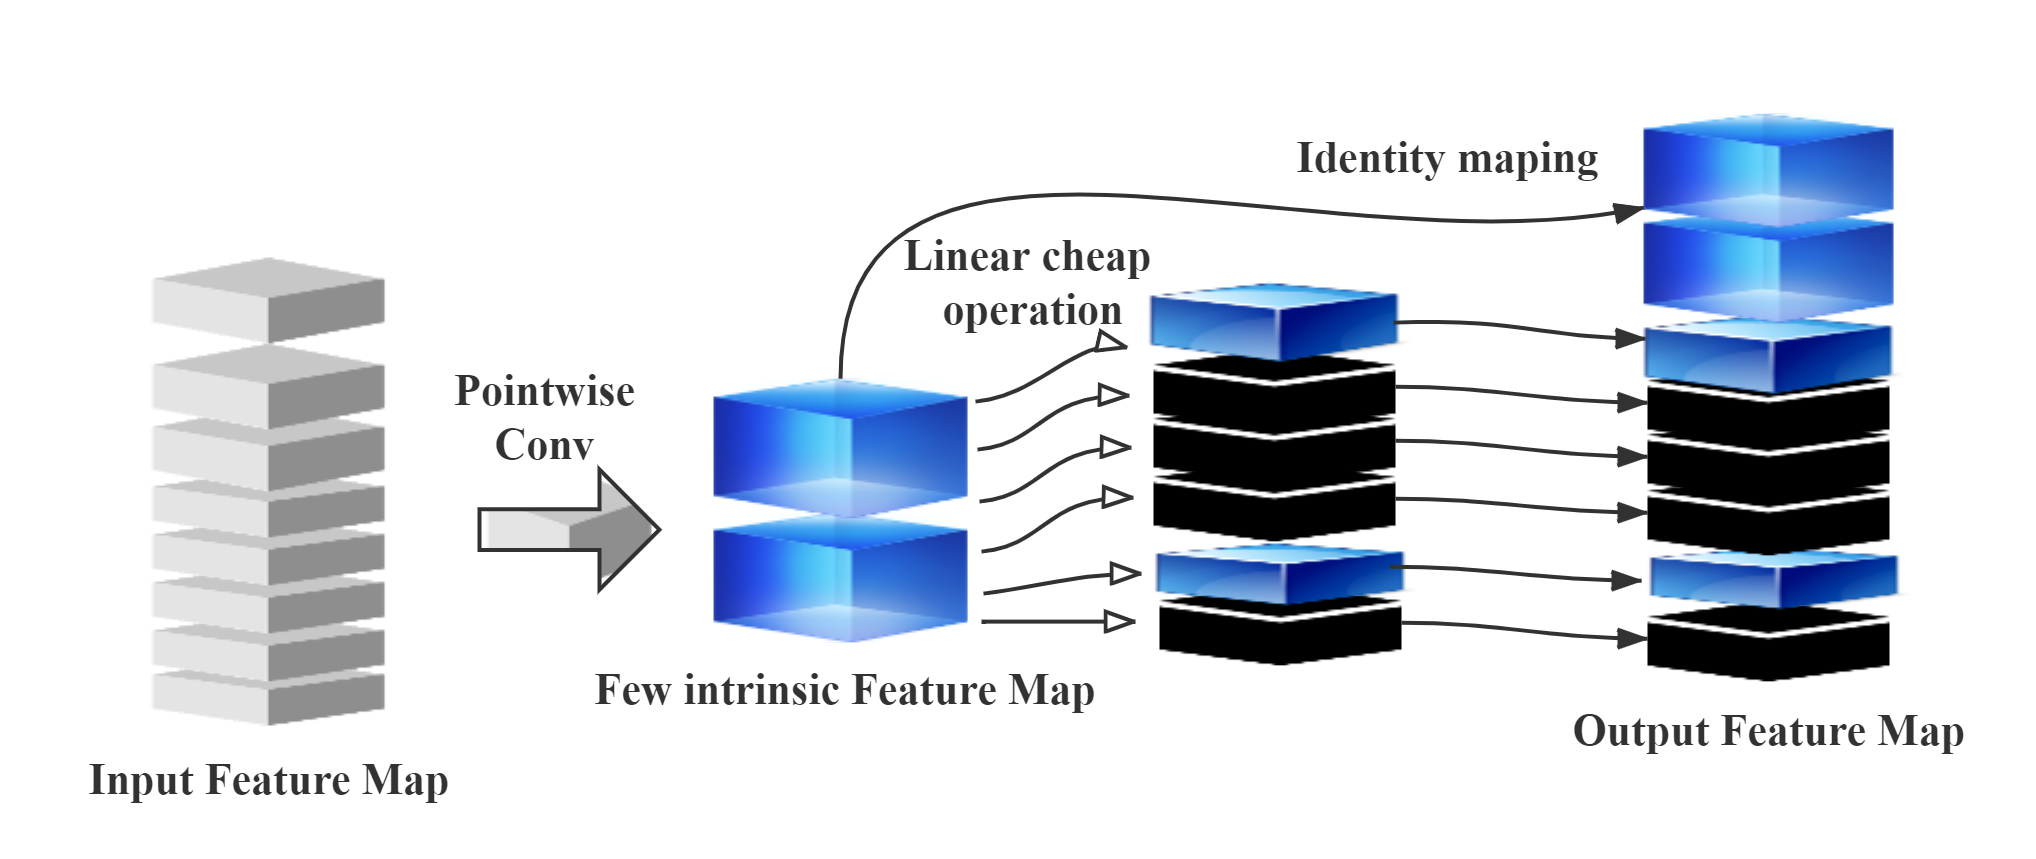
\includegraphics[width=\textwidth]{thesis-template-master/images/ghostmodule.png}
			
			\label{fig:cellnet}
		\end{subfigure}
	\end{center}
	\caption{\textbf{The ghost module layer in \cite{19}}. We only take point-wise convolution once to get a few intrinsic feature maps, and then we utilized the cheap linear transformation to generate a ghost map with a lower cost.}
	\label{fig:3.8}
\end{figure}

Unlike the Ghost module applied in GhostNet\cite{19}, we designed two kinds of new Ghost Modules for feature extraction and adopted the SE layers from Squeeze-and-Excitation Networks \cite{24} for enhancing useful features and balancing less inhibiting feature map. The first novel Ghost module inside Gbneck acts as an expansion layer, increasing the number of channels, while the second Ghost module reduces the number of channels to match the short-cut path. Then the inputs and the outputs of these two Ghost modules are concatenated by short-cut. We adopted batch normalization (BN) and ReLU non-linearity right after each layer as well\cite{19}, except that ReLU was not used after the second Ghost module, as suggested by MobileNetV2\cite{30}. In each novel Ghost Module, we only take point-wise convolution once to get a few intrinsic feature maps, then we utilized the cheap linear transformation such as depth-wise convolution or affine transformation and wavelet transformation, as suggested by GhostNet\cite{19}, here the depth-wise convolution was used.

\begin{figure}[h]
	\begin{center}
		\begin{subfigure}[b]{0.49\textwidth}
		    \centering
			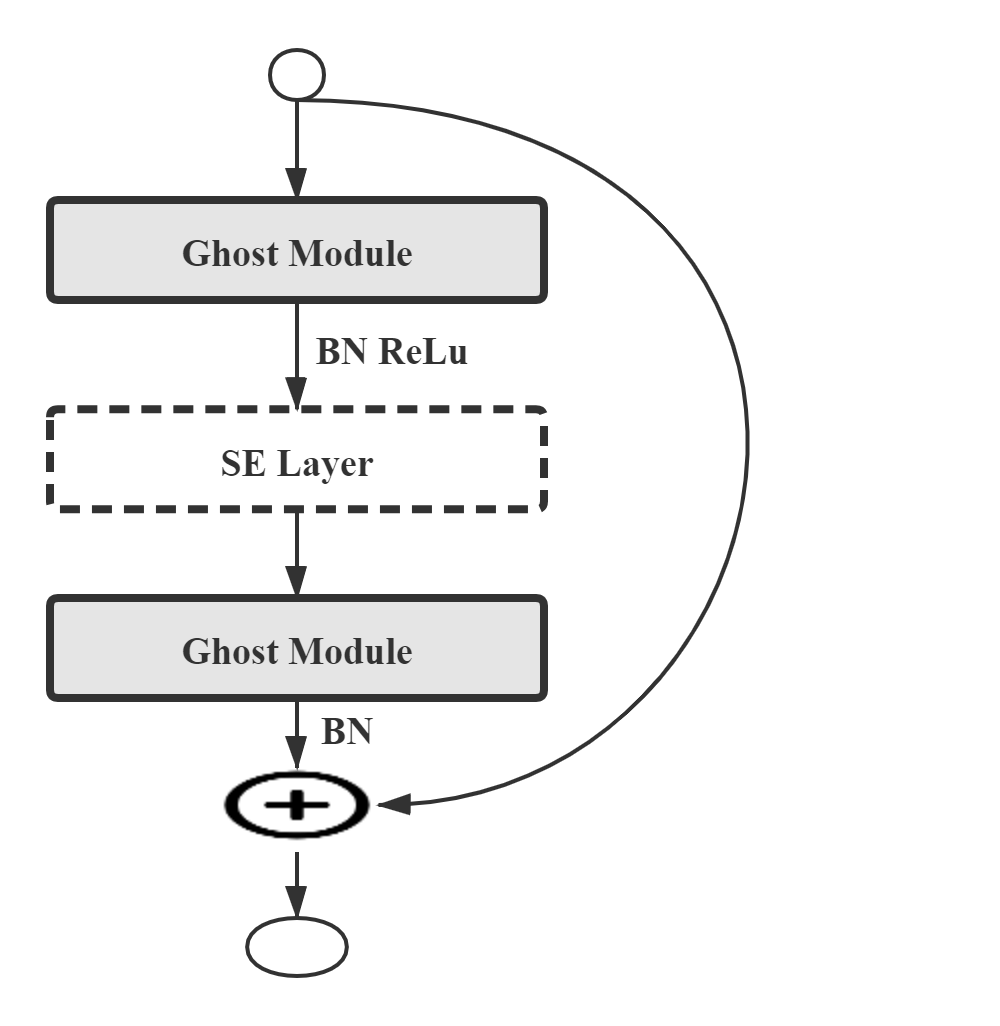
\includegraphics[width=\textwidth]{thesis-template-master/images/stride1 module.png}
			\caption{Stride = 1 SE = 0 G-bneck}
			\label{fig:cellnet}
		\end{subfigure}
		\begin{subfigure}[b]{0.49\textwidth}
		    \centering
			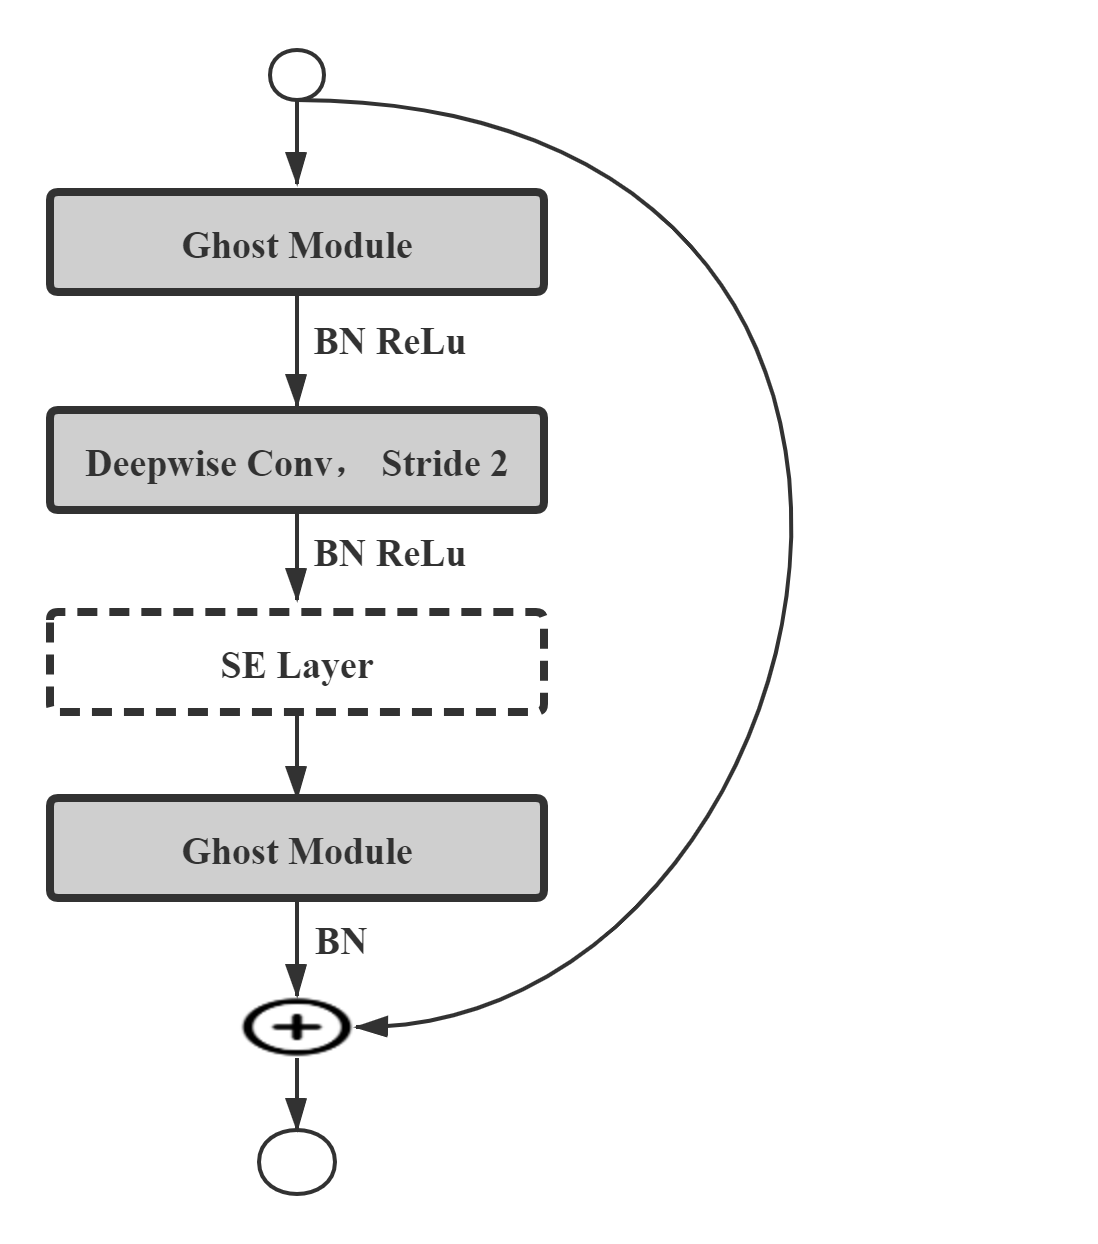
\includegraphics[width=\textwidth]{thesis-template-master/images/stride2 module.png}
			\caption{Stride = 2 SE = 0 G-bneck}
			\label{fig:cellnet}
		\end{subfigure}
	\end{center}
	\caption{\textbf{Two kind of Gbnecks we proposed for feature extraction}.We implement Stride = 1 to keep the output channel of the feature map, and Stride = 2 reduces the output channel while extracting information without losing much information. SE = 0 denotes not applying the SE layer.  The short-cut is used to correlate between the inputs and outputs of these two Ghost modules, as suggested by GhostNet, we achieve in the short-cut of Stride=2 G-bneck by a downsampling layer only single connection in short-cut of Stride =1 G-bneck.}
	\label{fig:3.9}
\end{figure}


\subsection{Squeeze-and-Excitation (SE Layer)} % (fold)
\label{sub:amet}

\textbf{Scaling inhibiting vs intrinsic features map.} Squeeze-and-Excitation (SE)\cite{24} adaptively recalibrates channel-wise feature responses by explicitly modeling inter-dependencies between channels.

SENet further proved that SE blocks bring significant improvements in performance for existing state-of-the-art CNNs with slight additional computational cost \cite{24}. 



\subsection{Analysis on complexities and necessities} % (fold)
\label{sub:dolor_sit}
Here, we extra analyze the profit on memory usage and theoretical speed-up by manipulating the Ghost module. In enhancement, we will draft the visual experiments. The theoretical speed-up ratio of $ \gamma $ of upgrading ordinary convolution with the Ghost module is equal to the following:

\begin{equation}
\begin{split}
\gamma $& = \frac{\left ( n\cdot {h}'\cdot {w}'\cdot c\cdot k\cdot k \right )}{\left (\frac{n}{s}\cdot {h}'\cdot {w}'\cdot c\cdot k\cdot k +\left ( s-1 \right )\cdot \frac{n}{s}\cdot {h}'\cdot {w}' \cdot d\cdot d \right )} \\
$&= \frac{c\cdot k\cdot k}{\frac{1}{s}\cdot c\cdot k\cdot k + \frac{s-1}{s}\cdot d\cdot d } \\
$&\approx \frac{s\cdot c}{s +c-1 } \\
$&\approx s $\label{speed}
\end{split}
\end{equation}

In Equation \eqref{speed}, ${h}' \cdot {w}' \cdot {n}$ represents  $n$ output feature maps with height ${h}'$, width ${w}'$, and $k \cdot k$, $d \cdot d$ stands for the convolution kernel filter and linear operation kernel size, respectively. And $m$ is the number of intrinsic feature maps, where $m < n$ because we only take few intrinsic feature maps and apply a series of cheap linear operations on each intrinsic feature to generate $s$ ghost features. It is also noteworthy that there are 1 ghost map adopted by identify mapping that indicates $s-1$. In total there are $\frac{n}{s} \cdot(s-1)$  linear operations. This leads to theoretically $s$ speed-up ratio.

More major feature maps will be generated by a linear operation based on a set of intrinsic feature maps instead of creating redundant data by point-wise convolution demands of a massive amount of parameters simultaneously. It furthermore partially explains that our net reaches the best performance on several benchmarks.
As far as we profoundly analyze each-layer-generated feature map by our net, we can additionally figure out the second factor: the artifacts appear in the image could also be learned by the neural network, which significantly affects the accuracy of the network, with the combination of AttentionNet segmentation techniques in cell image pre-processing, we can more focus on cell object rather than artifacts.


\begin{table}[htbp]
\centering

\scalebox{0.9}{
\begin{tabular}{@{}llllllll@{}}
\toprule
layer & Type    & Filters & Size/Stride           & Input      & Output     & \multicolumn{1}{l}{\#Expan} & SE \\ \midrule
0     & Conv2d  & 64      & 3\times3/2                 & 416\times416\times3  & 112\times112\times64 & -                                  & -  \\
1     & Maxpool & -       & 3\times3/2                 & 112\times112\times64 & 56\times56\times64   & -                                  & -  \\
2     & G-bneck & 64      & 3\times3/1                 & 56\times56\times64   & 56\times56\times64   & 64                                 & 0  \\
3     & G-bneck & 64      & 3\times3/1                 & 56\times56\times64   & 56\times56\times64   & 64                                 & 0  \\
4     & G-bneck & 64      & 3\times3/1                 & 56\times56\times64   & 56\times56\times64   & 128                                & 1  \\
5     & G-bneck & 128     & 3\times3/2                 & 56\times56\times64   & 28\times28\times128  & 256                                & 0  \\
6     & G-bneck & 128     & 3\times3/1                 & 28\times28\times128  & 28\times28\times128  & 512                                & 1  \\
7     & G-bneck & 256     & 3\times3/2                 & 28\times28\times128  & 14\times14\times256  & 1024                               & 0  \\
8     & G-bneck & 256     & 3\times3/1                 & 14\times14\times256  & 14\times14\times256  & 1024                               & 1  \\
9     & G-bneck & 512     & 3\times3/2                 & 14\times14\times256  & 7\times7\times512    & 1024                               & 0  \\
10    & Conv2d  & 512     & 1\times1/1                 & 7\times7\times512    & 7\times7\times512    & -                                  & -  \\
11    & Advpool & -       & 7\times7                   & 7\times7\times512    & 1\times1\times512    & -                                  & -  \\
12    & Conv2d  & 512     & 1\times1/1                 & 1\times1\times512    & 1\times1\times512    & -                                  & -  \\
13    & FC      & -       & \multicolumn{1}{c}{-} & 1\times1\times512    & 1000       & -                                  & -  \\ \bottomrule


\end{tabular}}
\caption{\textbf{CellNet Network Structure}. G-bneck denotes novel Ghostbottleneck that we designed. We use 8 Ghostbottleneck in corresponding to ResNet18 \cite{20} 16 feature extraction layers of point-wise convolution. We adopted 1:0:1:0:1:0 frequency of SE layer \cite{24} in corresponding to the stride frequency of 1:2:1:2:1:2 to satisfied that the re-scaling of less weight ghost map already executed before decrease of output channel.\#Expan means expansion size. }
\end{table}
































\chapter{Experiments}
\label{sec:examples}
In this chapter, we focus on experimentally evaluating our proposed two architectures. At the very beginning, we will introduce the standard evaluation metrics, such as Confusion Matrix, F1 Score, Area Under the ROC curve(AUC – ROC), Top-1 accuracy, mAP,  weights and FLOPs and so on. 

Followed by qualitative and quantitative results on two well-established benchmark data sets ( Cifar-10 \cite{21} for the approved classification task, Pneumonia dataset \cite{38} for biomedical classification task), we also contribute to the work of the establishing the first-ever Sezary Syndrome dataset benchmark, including the data acquisition, handling, aggregating and pre-processing with our AttentionNet to classifier data into the corresponding folder. Among the well-established benchmark, we also made the COVID-19 X-ray/CT image dataset while participating in the Kaggle challenge fighting against the COVID-19. We then report a state-of-the-art result on all these four data sets. We also provide detailed descriptions of the training and testing pipeline, including data pre-processing, training tricks and strategies, and network architectures used to obtain the final scores.

\section{Evaluation Metrics}
\label{sec:lorem}
In order to quantitatively evaluate the performance of the model, we define Evaluation metrics suit for our cases.

To start with our AttentionNet,  as described in chapter 3, the AttentionNet is based on classification task and follows the superiority of the architecture of Yolov3- tiny \cite{18}, therefore, there is generally established metric for evaluation, such as Confusion Matrix Precision and Recall, F1 Score, mAP,  the IOU and  Classification Loss. To compare our methods on the new dataset we established, we, therefore, adopted most of those evaluation schemes from the original YOLOv3\cite{33}. Moreover, combining Area Under the ROC curve leads to conclusive quality metrics paying attention to various aspects. 
In further, we acknowledge the resources limitation and time cost for software application in real scenarios usages, we then analyzed the time cost in different GPU availability and computation FLOPs.


\subsection{Confusion Matrix}
To make quantitative statements about the model of the CellNet, we mainly appropriated the  Confusion Matrix (TP, TN, FP, FN, Sensitivity, Accuracy), time complexity, weights of parameters, and the computation complexity FLOPs. 
Evaluation metrics are the means to perform this comparison, which is presented in the following paragraphs.

A confusion matrix is an $N \times N $ matrix, where $ N $ is the number of predicted classes. Because we possess a binary classification problem, we set then the $N=2$, and hence we get a $2 \times 2$ matrix. Here are a few definitions:


\begin{table}[h]
\centering
\scalebox{0.8}{
\begin{tabular}{|l|l|l|l|l|}
\hline
\multicolumn{2}{|c|}{\multirow{2}{*}{\textbf{}}}                                                & \multicolumn{2}{c|}{\textbf{Target}}                                                                                                  & \multirow{2}{*}{}    \\ \cline{3-4}
\multicolumn{2}{|c|}{}                                                                          & Positive                                                          & Negative                                                          &                      \\ \hline
\multirow{2}{*}{\textbf{\begin{tabular}[c]{@{}c@{}}Model\\ Prediction\end{tabular}}} & Positive & TP                                                                & FP                                                                & Precision (TP/(TP+FP)) \\ \cline{2-5} 
                                                                                     & Negative & FN                                                                & TN                                                                & Recall (TN/(FN+TN))   \\ \hline
\multicolumn{2}{|l|}{}                                                                          & \begin{tabular}[c]{@{}l@{}}Sensitivity \\ (TP/(TP+FN))\end{tabular} & \begin{tabular}[c]{@{}l@{}}Specificity \\ (TN/(FP+FN))\end{tabular} &                      \\ \hline

\end{tabular}}

\caption{\textbf{The illustration of  Confusion Matrix}. We will use the precision and recall as evaluation matrix in our experiments.}

\end{table}

The number of true positives ($TP$) constitutes how many data points of the ground truth class $c$ were correctly classified:


\begin{equation}
\begin{split}
TP\left ( Y_{p},Y_{g},c \right )=\sum_{x}^{}Y_{p}\left ( x,c \right )\times Y_{g}\left ( x, c \right )
\label{}
\end{split}
\end{equation}
where the ground truth class distribution $Y_{g} (x, c)$ and the predicted class distribution $Y_{p} (x, c)$ which both yield $1$ if the data point $x$  is classified as class $c$.

\begin{equation}
\begin{split}
TN\left ( Y_{p},Y_{g},c \right )=\sum_{x}^{}\left (1-Y_{p}\left ( x,c \right )  \right )\times \left ( 1-Y_{g}\left ( x,c \right ) \right ) 
\label{}
\end{split}
\end{equation}

The number of true negatives ($TN$) comprises how many data points not belonging to the ground truth class $c$ was correctly rejected by the predictor.

\begin{equation}
\begin{split}
FP\left ( Y_{p},Y_{g},c \right )=\sum_{x}^{}Y_{p}\left ( x,c \right )\times \left ( 1-Y_{g}\left ( x,c \right ) \right )
\label{}
\end{split}
\end{equation}

The number of false positives ($FP$) represents how many data points not belonging to the ground truth class c were wrongly classified by the predictor.
The final metric is the number of false negatives ($FN$) which represents how many data points of the ground truth class c were wrongly rejected by the predictor:
\begin{equation}
\begin{split}
FN\left ( Y_{p},Y_{g},c \right )=\sum_{x}^{}\left (1-Y_{p}\left ( x,c \right )  \right )\times Y_{g}\left ( x,c \right ) 
\label{}
\end{split}
\end{equation}


Another metric is precision, which measures the ratio between true positives and the overall number of class instantiations. Precision returns a probability estimate of how exact our predictor is, and it returns the proportion of positive cases that were correctly identified. Besides precision, there is the metric of recall, which is defined as the fraction of true positives to the overall positive samples. This estimates how complete a prediction is, as it generates the proportion of negative cases that were correctly identified.

In general, we are concerned with more than one of the above-defined metric.
A high precision rate, therefore, states that positive predictions are likely to be classified correctly. Contrastingly, the recall rate measures how complete a prediction is. Hence, a high recall rate means that a specific class's instantiations are likely to be detected in the dataset.

However, we favor a scalar value to create an ordered ranking of algorithms performing the same task. We thus condense both metrics into a single one. The $F$ score measures weights precision and recall according to a weighting factor such that recall has $ \beta $ times more weight than precision:
\begin{equation}
\begin{split}
F_{\beta }=\left ( 1+\beta ^{2} \right )\times \frac{precision\times recall}{\left (\beta ^{2}\times precision \right )+recall }
\label{}
\end{split}
\end{equation}

In the case of $ \beta = 1$, the $F_{1 }$ score is the harmonic mean between precision and recall.

Positively correlated to F score is the metric of intersection over union (IoU), which is prominent in the computer vision field and is used in the evaluation protocols across all tested datasets of this thesis.




\subsection{ROC curve and AUC (Area under Curve)}
The ROC (Receiver operating characteristic) curve is the plot between sensitivity and (1- specificity). As shown in Table 4.1, the sensitivity of a test is also called the true positive rate (TPR) and stands for the proportion of actual positive cases that are correctly identified. For example, a test that correctly identifies all positive samples in a panel is very sensitive. Another test that only detects 60 \% of the positive samples in the panel would be deemed to have lower sensitivity as it is missing positives and to give higher a false negative rate (FNR).

The specificity of a test, also referred to as the true negative rate (TNR), is the proportion of samples that test negative and are genuinely negative. For example, a test that identifies all healthy people as being negative for a particular illness is very specific. Another test that incorrectly identifies 30 \% of healthy people as having the condition would be deemed to be less specific, having a higher false-positive rate (FPR).

(1- specificity) is also known as the false-positive rate (FNR). On the other hand, the ROC curve is almost independent of the response rate because it has the two-axis coming out from columnar calculations of the confusion matrix.

\begin{figure}[h]
	\begin{center}
		\begin{subfigure}[b]{\textwidth}
		    \centering
			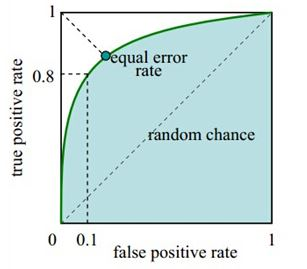
\includegraphics[width=0.4\textwidth]{thesis-template-master/images/ROC.JPG}
			\label{fig:cellnet}
		\end{subfigure}
	\end{center}
	\caption{\textbf{ROC (Receiver operating characteristic) curve}. $x$ axis in ROC curve represents FPR, or 1-TNR, or 1-Specificity. The higher the FPR, the more actual negative categories in the predicted positive category. On the other hand, $y$ axis in the ROC curve represents TPR or, by other words, Sensitivity. The higher the TPR, the more actual positive categories in the predicted positive category.}
	\label{fig:4.1}
\end{figure}
Our idea objective will be TPR=1 and FPR=0, which is the (0,1) point in the figure, so the closer the ROC curve is to the (0,1) point, the better it deviates from the diagonal of 45 degrees, and the higher the Sensitivity and Specificity, the more effective.
The numerator and denominator of both x and y-axis will change on a similar scale in the response rate shift.

The most significant advantage of utilizing the ROC curve is that it is independent of the variation in the proportion of responders. This statement will get more explicit in the following sections.

As a numerical value, AUC(Area under Curve) can directly evaluate the classifier's quality, and it calculates the area under the ROC curve, which varies from 0 and 1.  A test with perfect accuracy has an AUC of 1.

The interpretation of the AUC is the average value of Sensitivity for all possible values of specificity. To more clearer, we illustrated with a binary classification problem, by randomly given a positive sample and a negative sample. AUC represents the probability of the classifier predicting positive samples is higher than the probability of the classifier predicting negative samples.%AUC评估的是随机给定一个正样本和一个负样本,模型对正样本的预测概率大于模型对于负样本预测概率的概率


\subsection{Top N accuracy }
Top N accuracy is not any different metric, but it is just standard accuracy of the target class being equal to any of the N most probable classes predicted by the classification model. Top 1 accuracy is the accuracy in which the target class matches the most probable classes predicted by the model, which is the same as our standard accuracy. Top 2 accuracy is the accuracy where target class matches with any one of the 2 most probable classes predicted by the model. Moreover, accordingly, the Top 3 accuracy is the accuracy where target class matches with any one of the 3 most probable classes predicted by the model. In the same way, we can measure the top 4, top 5, top 6, and so on.


We illustrate both metrics in the following examples considering classifying records into respective animals (dog, cat, lion, tiger, and elephant). The following table shows the target class and the predicted class of 6 records.
For instance, if the test target class is given dog, the target class under the Top 1 accuracy circumstance is unmatched with the most probable classes predicted by the model{Cat}. Therefore, this can be recognized as false prediction, leading to 50\% Top 1 accuracy.
On the other hand, the target class under the Top 2 accuracy circumstance matches with the most two probable classes predicted by the model{Cat, Dog}.because only one match, we can count them as positive prediction, it leads to 83\% on Top  2  accuracy.
\begin{table}[h]
\centering

\begin{tabular}{@{}cccc@{}}

\toprule
\multicolumn{2}{c}{Top-1 accuracy: 0.5} & \multicolumn{2}{c}{Top-2 accuracy: 0.83} \\ \midrule
Test Target class    & Prediction      & Test Target class   & Prediction         \\
Dog                  & \{Cat\}         & Dog                 & \{Cat, Dog\}       \\
Elephant             & \{Elephant\}    & Elephant            & \{Elephant, Cat\}  \\
Lion                 & \{Tiger\}       & Lion                & \{Tiger, Cat\}     \\
Dog                  & \{Dog\}         & Dog                 & \{Dog, Lion\}      \\
Lion                 & \{Lion\}        & Lion                & \{Lion, Cat\}      \\
Tiger                & \{Cat\}         & Tiger               & \{Cat, Tiger\}     \\ \bottomrule


\end{tabular}

\caption{\textbf{The illustration of Top 1 accuracy and Top 2 accuracy}. As Table illustrated, we will obtain an accuracy of 50\% on Top 1 accuracy and 83\% on Top 2 accuracy. }
\end{table}


As Table 4.2 illustrates, we will obtain an accuracy of 50\%, when we are taking the Top 1 accuracy into evaluation metrics, which is not satisfying. As soon as we take into consideration of the accuracy where target class matches with any one of the two most probable classes predicted by the model, as the second column demonstrated, we will be getting an accuracy of 83\%, which is a significant increase compared to the previous one. It is the basic intuition behind the Top N accuracy, which is especially applicable for the mutil-class objects prediction tasks.





\section{Sezary Syndrome Dataset}
\label{sec:lorem}

\begin{figure}[h]
	\begin{center}
		\begin{subfigure}[b]{\textwidth}
		    \centering
			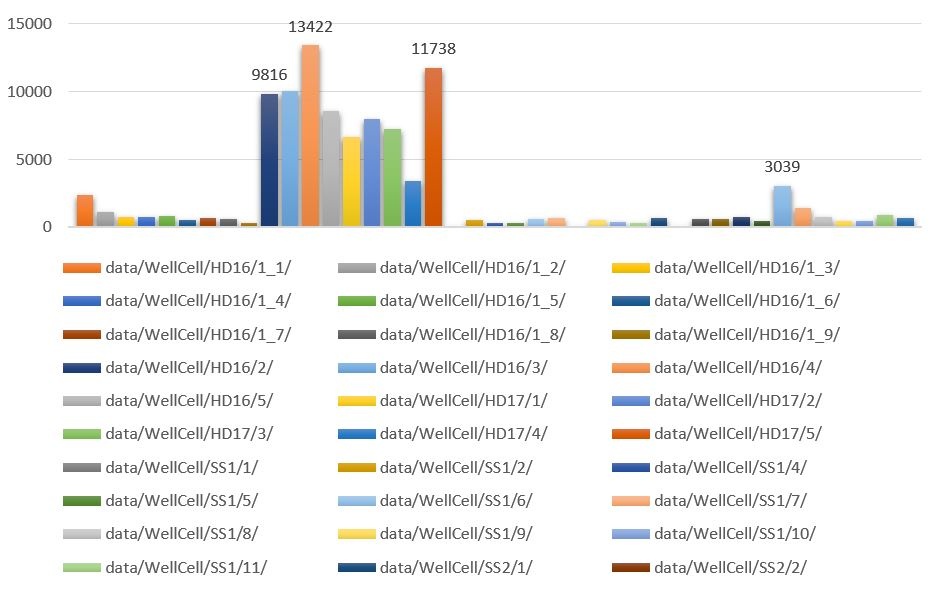
\includegraphics[width=0.9\textwidth]{thesis-template-master/images/wellcellSezary dataset.JPG}
			\label{fig:cellnet}
		\end{subfigure}
	\end{center}
	\caption{\textbf{Wellcell dataset on Sezary dataset}. In total we had Well cell data:$HD16:49787+ HD17:37009+SS1:5250+SS2:10852= 102,898$.}
	\label{fig:4.2}
\end{figure}

\begin{figure}[h]
	\begin{center}
		\begin{subfigure}[b]{\textwidth}
		    \centering
			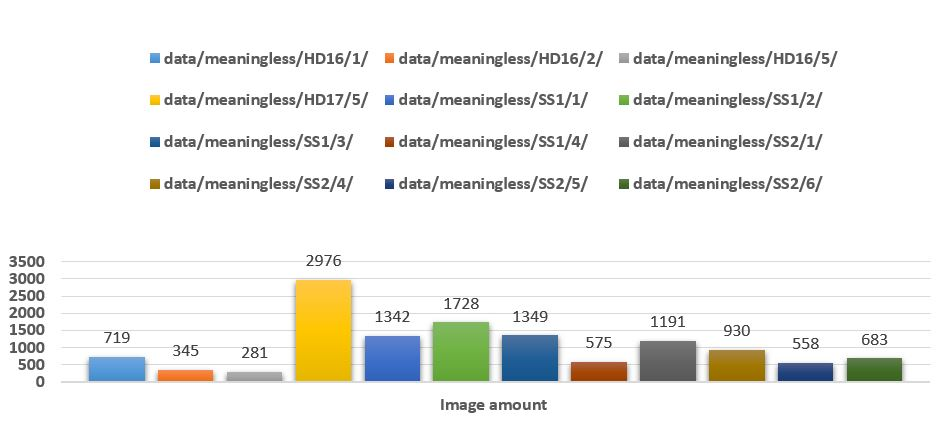
\includegraphics[width=0.9\textwidth]{thesis-template-master/images/noiseofSezarySyndrome.JPG}
			\label{fig:cellnet}
		\end{subfigure}
	\end{center}
	\caption{\textbf{Noise dataset of Sezary Syndrome}.We had noise data: 12,695.}
	\label{fig:4.3}
\end{figure}

\subsection{The introduction of Sezary Syndrome Dataset}
Sezary syndrome is an aggressive form of cutaneous T-cell lymphoma, which is a group of disorders that occur when T-cells (a type of white blood cell) become cancerous and affect the skin\cite{Alain}. Moreover, it corresponds to 3\% of all cutaneous lymphomas, and it is characterized by a triad of manifestations: erythroderma with pruritus, limphonodomegalia, and atypical circulating lymphocytes (referred to as Sézary or Lutzner cells). Associated clinical manifestations include lagophthalmos, alopecia, palmoplantar hyperkeratosis, and onycodystrophy \cite{Yamashita}.


\begin{figure}[ht]
	\begin{center}
		\begin{subfigure}[b]{0.25\textwidth}
			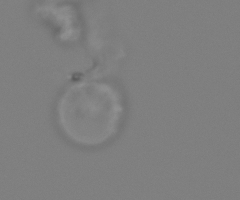
\includegraphics[width=\textwidth]{thesis-template-master/images/noisefortest (106).png}
			\label{fig:Debris}
		\end{subfigure}
		\begin{subfigure}[b]{0.25\textwidth}
			\reflectbox{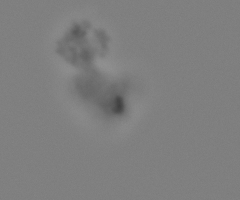
\includegraphics[width=\textwidth]{thesis-template-master/images/noisefortest (107).png}}
			\label{fig:Out of Focus}
		\end{subfigure}
		\begin{subfigure}[b]{0.25\textwidth}
			\reflectbox{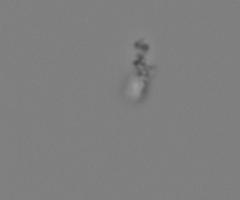
\includegraphics[width=\textwidth]{thesis-template-master/images/noisefortest (47).png}}
			\label{fig:Lighting Artifacts}
		\end{subfigure}
		\begin{subfigure}[b]{0.25\textwidth}
			\reflectbox{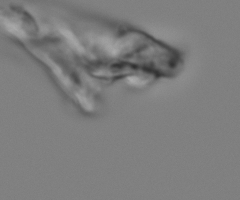
\includegraphics[width=\textwidth]{thesis-template-master/images/noisefortest (66).png}}
			\label{fig:Outside FOV}
		\end{subfigure}
		\begin{subfigure}[b]{0.25\textwidth}
			\reflectbox{\includegraphics[width=\textwidth]{thesis-template-master/images/noisefortest (69).png}}
			\label{fig:Contaminated}
		\end{subfigure}
		\begin{subfigure}[b]{0.25\textwidth}
			\reflectbox{\includegraphics[width=\textwidth]{thesis-template-master/images/noisefortest (91).png}}
			\label{fig:Good Cell}
		\end{subfigure}
		\begin{subfigure}[b]{0.25\textwidth}
			\reflectbox{\includegraphics[width=\textwidth]{thesis-template-master/images/noisefortest (93).png}}
			\label{fig:Good Cell}
		\end{subfigure}
		\begin{subfigure}[b]{0.25\textwidth}
			\reflectbox{\includegraphics[width=\textwidth]{thesis-template-master/images/noisefortest (87).png}}
			\label{fig:Good Cell}
		\end{subfigure}
				\begin{subfigure}[b]{0.25\textwidth}
			\reflectbox{\includegraphics[width=\textwidth]{thesis-template-master/images/ss5 (1).png}}
			\label{fig:Good Cell}
		\end{subfigure}
	\end{center}
	\caption{\textbf{Meaningless noise images from Sezary Syndrome data set}.  The six typical noise images introduced in \eg\reffig{1.1}. In total, we had noise data: 12,695.}
	\label{fig:4.4}
\end{figure}

Sezary syndrome symptoms are described by a widespread red rash that may reach most of the body, malignant T cells (called Sezary cells) in the blood, and abnormally expanded lymph nodes. Additional symptoms may include severe itchiness, scaling plus peeling of the skin, fever, weight loss, hair loss, outward turning of the eyelids (ectropion). According to \cite{10.1182/blood-2004-09-3502}\cite{20001195667}, the presence of the Sezary syndrome is aggressive with a median survival of 1 to 5 years. Moreover, the exact cause of Sezary syndrome is currently undiscovered. Medication differs based on the types and symptoms present in each person and the severity of the condition.\cite{Yamashita}.

A diagnosis of Sezary syndrome is often suspected in people with particular types and symptoms. Additional testing can then be ordered to confirm the diagnosis. It may include: A skin biopsy, A complete blood count, Peripheral blood smear, Immunophenotyping, T-cell receptor (TCR) gene rearrangement test, and Flow cytometry \cite{Alain}.


\begin{figure}[ht]
	\begin{center}
		\begin{subfigure}[b]{0.25\textwidth}
			\includegraphics[width=\textwidth]{thesis-template-master/images/hd7 (80).png}
			\label{fig:Debris}
			\caption{HD cell}
		\end{subfigure}
		\begin{subfigure}[b]{0.25\textwidth}
			\reflectbox{\includegraphics[width=\textwidth]{thesis-template-master/images/hd7 (107).png}}
			\label{fig:Out of Focus}
			\caption{HD cell}
		\end{subfigure}
		\begin{subfigure}[b]{0.25\textwidth}
			\reflectbox{\includegraphics[width=\textwidth]{thesis-template-master/images/hd7 (102).png}}
			\label{fig:Lighting Artifacts}
			\caption{HD cell}
		\end{subfigure}
		\begin{subfigure}[b]{0.25\textwidth}
			\reflectbox{\includegraphics[width=\textwidth]{thesis-template-master/images/ss5 (135).png}}
			\label{fig:Outside FOV}
			\caption{SS cell}
		\end{subfigure}
		\begin{subfigure}[b]{0.25\textwidth}
			\reflectbox{\includegraphics[width=\textwidth]{thesis-template-master/images/ss5 (120).png}}
			\label{fig:Contaminated}
			\caption{SS cell}
		\end{subfigure}
		\begin{subfigure}[b]{0.25\textwidth}
			\reflectbox{\includegraphics[width=\textwidth]{thesis-template-master/images/ss5 (24)}}
			\label{fig:Good Cell}
			\caption{SS cell}
		\end{subfigure}
		
	\end{center}
	\caption{\textbf{Well cell images from Sezary Syndrome data set}. Only Well cell images from the Sezary Syndrome data set can be analyzed in the classification task. As shown in the figure, the morphological characteristics can be even hardly distinguished by experts, which partly explains the unsatisfied classification accuracy of the neural network. In total, we had well cell data: 102,898.}
	\label{fig:4.5}
\end{figure}

Based on the previously manually folder-labeled image, we manipulated the second round of filtering, because of the impurity of the data set. Because we do not allow the cell folder contains noise data, so we manually checked for the whole data set again and deleted those raw images, the following data is the newest version of the folder(Seen \eg\reffig{4.2} and \eg\reffig{4.3}). 



\subsection{AttentionNet on Sezary Sydrome Dataset}

\begin{table}[t]
\scalebox{0.5}{
\begin{tabular}{@{}ccl@{}}
\toprule
Configuration hyperparameter         & Value                                                                                                & Annotation                                                                                                                                                                                                                                                                                                                                                                                             \\ \midrule
\multicolumn{1}{|c|}{batch}          & \multicolumn{1}{c|}{64}                                                                              & \multicolumn{1}{l|}{Update parameters every batch of 64 samples}                                                                                                                                                                                                                                                                                                                                       \\ \midrule
\multicolumn{1}{|c|}{subdivisions}   & \multicolumn{1}{c|}{1}                                                                               & \multicolumn{1}{l|}{\begin{tabular}[c]{@{}l@{}}The batch will be divided by 1 to decrease GPU VRAM requirements \\ as we are using ETH Leonhard we donot facing the GPU resources limitations\end{tabular}}                                                                                                                                                                                            \\ \midrule
\multicolumn{1}{|c|}{height}         & \multicolumn{1}{c|}{416}                                                                             & \multicolumn{1}{l|}{The width of input figure}                                                                                                                                                                                                                                                                                                                                                         \\ \midrule
\multicolumn{1}{|c|}{width}          & \multicolumn{1}{c|}{416}                                                                             & \multicolumn{1}{l|}{The height of input figure}                                                                                                                                                                                                                                                                                                                                                        \\ \midrule
\multicolumn{1}{|c|}{channels}       & \multicolumn{1}{c|}{3}                                                                               & \multicolumn{1}{l|}{\begin{tabular}[c]{@{}l@{}}The channels of input training images,\\ as our image is here RGB image, therefore, we set here 3\end{tabular}}                                                                                                                                                                                                                                         \\ \midrule
\multicolumn{1}{|c|}{momentum}       & \multicolumn{1}{c|}{0.9}                                                                             & \multicolumn{1}{l|}{\begin{tabular}[c]{@{}l@{}}For the poorly conditioned Hessian matrix problem \\ (intuitively, the gradient is highly sensitive to certain directions of the parameter space)\\ usually set 0.5, 0.9, or 0.99, which means the maximum speed is \\ 2 times, 10 times, 100 times the algorithm of SGD\end{tabular}}                                                                  \\ \midrule
\multicolumn{1}{|c|}{decay}          & \multicolumn{1}{c|}{0.0005}                                                                          & \multicolumn{1}{l|}{Regularization term of weight decay  to prevent overfitting}                                                                                                                                                                                                                                                                                                                       \\ \midrule
\multicolumn{1}{|c|}{angle}          & \multicolumn{1}{c|}{0}                                                                               & \multicolumn{1}{l|}{Generate more training samples by rotation}                                                                                                                                                                                                                                                                                                                                        \\ \midrule
\multicolumn{1}{|c|}{saturation}     & \multicolumn{1}{c|}{1.5}                                                                             & \multicolumn{1}{l|}{Generate more training samples by adjusting saturation}                                                                                                                                                                                                                                                                                                                            \\ \midrule
\multicolumn{1}{|c|}{exposure}       & \multicolumn{1}{c|}{1.5}                                                                             & \multicolumn{1}{l|}{Generate more training samples by adjusting exposure}                                                                                                                                                                                                                                                                                                                              \\ \midrule
\multicolumn{1}{|c|}{hue}            & \multicolumn{1}{c|}{.1}                                                                              & \multicolumn{1}{l|}{Generate more training samples by adjusting hue}                                                                                                                                                                                                                                                                                                                                   \\ \midrule
\multicolumn{1}{|c|}{learning rate}  & \multicolumn{1}{c|}{0.001}                                                                           & \multicolumn{1}{l|}{\begin{tabular}[c]{@{}l@{}}Initial learning rate, The learning rate determines how fast the parameter moves to the optimal solution. \\ If it is too large, it may cross the optimal value and cause the model to fail to converge. \\ Otherwise if it is too small, the algorithm cannot converge for a long time \\ and it is easy to fall into the local optimal.\end{tabular}} \\ \midrule
\multicolumn{1}{|c|}{max batches}    & \multicolumn{1}{c|}{500200}                                                                          & \multicolumn{1}{l|}{Stop learning after training reaches max\_batches}                                                                                                                                                                                                                                                                                                                                 \\ \midrule
\multicolumn{1}{|c|}{policy}         & \multicolumn{1}{c|}{steps}                                                                           & \multicolumn{1}{l|}{\begin{tabular}[c]{@{}l@{}}The policies for adjusting the learning rate are as follows:\\ CONSTANT, STEP, EXP, POLY, STEPS, SIG, RANDOM\end{tabular}}                                                                                                                                                                                                                              \\ \midrule
\multicolumn{1}{|c|}{steps}          & \multicolumn{1}{c|}{400000,450000}                                                                   & \multicolumn{1}{l|}{Adjust the learning rate according to batch\_num}                                                                                                                                                                                                                                                                                                                                  \\ \midrule
\multicolumn{1}{|c|}{scales}         & \multicolumn{1}{c|}{.1,.1}                                                                           & \multicolumn{1}{l|}{The rate of change in learning rate, cumulatively multiplied}                                                                                                                                                                                                                                                                                                                      \\ \midrule
\multicolumn{1}{|c|}{mask}           & \multicolumn{1}{c|}{1,2,3,4,5,67,8,9}                                                                & \multicolumn{1}{l|}{Yolo Output Layer will select different three anchor box set}                                                                                                                                                                                                                                                                                                                      \\ \midrule
\multicolumn{1}{|c|}{anchors}        & \multicolumn{1}{c|}{\begin{tabular}[c]{@{}c@{}}38,39 50,53\\ 51,67 71,78\\ 84,83 99,95\end{tabular}} & \multicolumn{1}{l|}{\begin{tabular}[c]{@{}l@{}}The prior prediction box learned from our KMeans++cluster \\ one set contains two value (w,h)\end{tabular}}                                                                                                                                                                                                                                             \\ \midrule
\multicolumn{1}{|c|}{classes}        & \multicolumn{1}{c|}{2}                                                                               & \multicolumn{1}{l|}{The number of object classes that the network needs to classifier}                                                                                                                                                                                                                                                                                                                 \\ \midrule
\multicolumn{1}{|c|}{num}            & \multicolumn{1}{c|}{6}                                                                               & \multicolumn{1}{l|}{Each grid cell predicts \#num number of bounding boxes}                                                                                                                                                                                                                                                                                                                            \\ \midrule
\multicolumn{1}{|c|}{jitter}         & \multicolumn{1}{c|}{0.3}                                                                             & \multicolumn{1}{l|}{Increase noise by jitter to suppress overfitting}                                                                                                                                                                                                                                                                                                                                  \\ \midrule
\multicolumn{1}{|c|}{ignore\_thresh} & \multicolumn{1}{c|}{0.7}                                                                             & \multicolumn{1}{l|}{The parameter determines whether the IOU error needs to be calculated  in the cost function}                                                                                                                                                                                                                                                                                       \\ \midrule
\multicolumn{1}{|c|}{truth\_thresh}  & \multicolumn{1}{c|}{1}                                                                               & \multicolumn{1}{l|}{The size of the IOU threshold involved in the calculation}                                                                                                                                                                                                                                                                                                                         \\ \midrule
\multicolumn{1}{|c|}{random}         & \multicolumn{1}{c|}{1}                                                                               & \multicolumn{1}{l|}{Multi-scale training is enabled. Otherwise, the training size of image is the same as the input size}                                                                                                                                                                                                                                                                              \\ \bottomrule
\end{tabular}}
\caption{ \textbf{AttentionNet configuration files (.cfg) }. As shown in the evaluation table, we will present the training hyper-parameters that we chose in detail and explain why we set like that.}
\end{table}


\subsubsection{Implementation and Hyper-parameters}

\textbf{Preparing dataset.}  Ere begins to train; we prepare the data for object detection. We used the LabelImg tool to formulate the expert-defined good cell/noise contours. In this tool, we can make our data in two different formats: XML and txt. For the suggestion of original YOLOv3\cite{33}, we used txt format. We further wrote a function (xmltotxt.py) that can convert the XML format to txt format. 

Machine learning training procedure involves the principal splitting the data randomly into two sets. Using our (filtertrainandtest.py) script, we can split the test / train data set into user-defined distribution. Train set: this is the part of the data on which we train the model. Test set: this is the part of the data on which we test our model. Typically, this is 70\%/30\% of the data. No image should be part of both the train and the test set.

Then we create two files noted train.txt and test.txt. These files must save the path of train and test images in the data set line by line. Train.txt should have the formal: $(data/images/imagenames.png)$, and Test.txt should have the formal $(data/images/imagenames.png)$.

Because of supervised-learning, we should additionally generate (./image) and (. /labels) folder accordingly. Moreover, the label file and the image should have an identical filename. It can be guarantee by our script (xmltotxt.py).

\textbf{Preparing AttentionNet configuration files}. YOLOv3 \cite{33} needs certain specific files to know how and what to train. We must create these three files(.data, .names, and .cfg) and we explained those configuration hyperparameters in the above Table 4.3.\\



\subsubsection{Evaluated performances}
We train 1000 epochs and input 857 instance level labeled images, set up 772(90\%) image for train set, and 85 images for the test. For Training image: 772 images consists of 274 noise images, 144 HD Cell images, and 439 SS cell images. Val image: 85 images. In addition, we test the trained model on 723 new images as well.


\begin{table}[t]
\centering
\scalebox{0.6}{
\begin{tabular}{@{}clccc@{}}
\toprule
\multicolumn{1}{c}{\textbf{Evaluation matrix}} & \textbf{\begin{tabular}[c]{@{}c@{}}500 epochs\\ +450 train images \\ +YOLOv3 tiny\end{tabular}}                     & \textbf{\begin{tabular}[c]{@{}c@{}}1000 epochs\\ +450 train images\\ +YOLOv3 tiny\end{tabular}}                                     & \textbf{\begin{tabular}[c]{@{}c@{}}1000 epochs\\ +450 train images\\ +Circle detection\\ +YOLOv3 tiny\end{tabular}}                                               \\ \midrule
TP(HD Cell be detected as Cell)                & 193/308=0.633                                                                                                       & 0.6558                                                                                                                              & 0.56                                                                                                                                                              \\
TP(SS Cell be detected as Cell)                & 166/306=0.5424                                                                                                      & 0.6078                                                                                                                              & 0.4314                                                                                                                                                            \\
FP(Noise be detected as Cell)                  & 0                                                                                                                   & 1                                                                                                                                   & 0                                                                                                                                                                 \\
TN(Noise be detected as Noise)                 & 82/109=0.7523                                                                                                       & 0.871559                                                                                                                            & 0.6605                                                                                                                                                            \\
Image No Label                                 & 300/723=41.49\%                                                                                                     & 33.05\%                                                                                                                             & 47.72\%                                                                                                                                                           \\
mAP                                            & 0.376                                                                                                               & 0.551                                                                                                                               & 0.551                                                                                                                                                             \\
Time Cost(s)                                   & 236.344                                                                                                             & 16.344                                                                                                                              & 475.65                                                                                                                                                            \\ \midrule
\textbf{Evaluation matrix}                     & \textbf{\begin{tabular}[c]{@{}c@{}}1000 epochs\\ +850 train images\\ +Circle detection\\ +YOLOv3 tiny\end{tabular}} & \textbf{\begin{tabular}[c]{@{}c@{}}1000 epochs\\ +850 train images\\ +$26\times26$, $52\times52$  YOLOversion\\ +KMean++ clustering\end{tabular}} & \textbf{\begin{tabular}[c]{@{}c@{}}1000 epochs\\ +1400 train images\\ +$26\times26$, $52\times52$ YOLOversion\\ +Circle detection\\ +KMean++clustering \\ +GBCIOU\end{tabular}} \\ \midrule
TP(HD Cell be detected as Cell)                & 0.95129                                                                                                             & 0.9123                                                                                                                              & 0.8571                                                                                                                                                            \\
TP(SS Cell be detected as Cell)                & 0.9738                                                                                                              & 0.9117                                                                                                                              & 0.8497                                                                                                                                                            \\
FP(Noise be detected as Cell)                  & 12                                                                                                                  & 10                                                                                                                                  & 11                                                                                                                                                                \\
TN(Noise be detected as Noise)                 & 0.8073                                                                                                              & 0.6605                                                                                                                              & 0.587                                                                                                                                                             \\
Image No Label                                 & 1.93\%                                                                                                              & 11.20\%                                                                                                                             & 17.1\%                                                                                                                                                            \\
mAP                                            & 0.881                                                                                                               & 0.7255                                                                                                                              & 0.53                                                                                                                                                              \\
Time Cost(s)                                   & 15.674                                                                                                              & 284.467                                                                                                                             & 266.36                                                                                                                                                            \\ \bottomrule
\end{tabular}}
\caption{\textbf{Evaluation of different designs on Sezary Syndrome Dataset}}
\end{table}


\begin{figure}[t]
	\begin{center}
		\begin{subfigure}[c]{0.6\textwidth}
			\includegraphics[width=\textwidth]{thesis-template-master/images/An illustration test performance of CellYolo best weight.png}
			\label{fig:Debris}
			\caption{val Wellcell dataset}
		\end{subfigure}
		\begin{subfigure}[c]{0.6\textwidth}
			\includegraphics[width=\textwidth]{thesis-template-master/images/An illustration test performance of CellYolo best weight2.png}
			\label{fig:Out of Focus}
			\caption{val Noise dataset}
		\end{subfigure}
		
	\end{center}
	\caption{ \textbf{Detection Performance on val dataset with AttentionNet best weight}. As seen, the well cells are well recognized and ideally located as well. The main problem lay on the noise data, as we have seen the recognition is well-done even for different scale artifacts.}
	\label{fig:4.7}
	
\end{figure}

\begin{figure}[h]
\begin{center}
\includegraphics[width=\textwidth]{thesis-template-master/images/cellyolo best weight based on manually labeled 1500 images.png}
\label{fig:cellnet}
\end{center}
\caption{\textbf{The demonstration of train performance of AttentionNet best weight based on manually labeled 1500 images}. The P-value is nearly 85\%, and the F1 value is also quite well, the mAP@0.5 reaches nearly 88\%.}
\end{figure}

\begin{figure}[t]
	\begin{center}
		\begin{subfigure}[b]{0.25\textwidth}
			\includegraphics[width=\textwidth]{thesis-template-master/images/bestweightoncell.jpg}
			\label{fig:Debris}
			\caption{well cell}
		\end{subfigure}
		\begin{subfigure}[b]{0.25\textwidth}
			\includegraphics[width=\textwidth]{thesis-template-master/images/bestweightoncell2.jpg}
			\label{fig:Out of Focus}
			\caption{well cell}
		\end{subfigure}
		\begin{subfigure}[b]{0.25\textwidth}
			\includegraphics[width=\textwidth]{thesis-template-master/images/bestweightoncell3.png}
			\label{fig:Lighting Artifacts}
			\caption{well cell}
		\end{subfigure}
	
		\begin{subfigure}[b]{0.25\textwidth}
			\includegraphics[width=\textwidth]{thesis-template-master/images/bestweightonnoise1.jpg}
			\label{fig:Contaminated}
			\caption{noise cell}
		\end{subfigure}
		\begin{subfigure}[b]{0.25\textwidth}
			\includegraphics[width=\textwidth]{thesis-template-master/images/bestweightonnoise2.jpg}
			\label{fig:Good Cell}
			\caption{noise cell}
		\end{subfigure}
		\begin{subfigure}[b]{0.25\textwidth}
			\includegraphics[width=\textwidth]{thesis-template-master/images/bestweightonnoise3.jpg}
			\label{fig:Good Cell}
			\caption{noise cell}
		\end{subfigure}
	\end{center}
	\caption{ \textbf{Segmentation performance with AttentionNet best weight, GBCIOU and Circle segmentation}. The confidence score reaches up to 0.86 out of 1, and the segmentation performance for both well cell and noise close semantic level.}
	\label{fig:4.8}
\end{figure}

As table 4.4 illustrates, we conduct a thorough evaluation study on different design to support our claims that
(1)We achieve the current best weight based on 1000 epochs with nearly manually labeled 850 representative Noise and Well cell images, add Circle detect and segmentation in the final phase, and use YOLOv3-tiny \cite{18} two YOLO output layers architecture;
(2)The quantity of training image does not play a key role, but the training epochs contribute to the overall  performance;
(3)YOLO output tensors as a means of different target detectors individually contribute to classification and detection performance of different customer dataset;
(4)The combinations of different functions we designed, including GBCIOU or KMeans++ in pre-processing and novel architecture, enable us efficiently detect noise/well cell and final finishing segmentation at a very lower time cost.


\subsection{CellNet on Sezary Sydrome Dataset}

\subsubsection{Implementation and Hyper-parameters}
Here, we will give complete information on which models we derive from our proposed family of CellNet. Moreover, we discuss the training and testing pipeline, including pre-computation and augmentation steps. Our models are implemented in PyTorch and trained on an ETH Zurich Leonhard Cluster for at least 200 epochs. We refer to Chapter 5 for detailed ablation studies on the architectural components and focus on comparing current state-of-the-art methods in this chapter.

We train the network end-to-end by minimizing the cross-entropy loss using the SGD optimizer with an initial learning rate of 0.1 and setting the learning rate to the initial LR decayed by 10 every 30 epochs and weight-decay of 1e-4  with a batch size of 256.

\begin{table}[b]
\scalebox{0.55}{
\begin{tabular}{@{}ccl@{}}
\toprule
\textbf{Hyperparameter}                      & \textbf{Value}                                                                                                              & \textbf{Annotation}                                                                                                                                                                                                                                                                                                                                                                                       \\ \midrule
\multicolumn{1}{|c|}{batch}                  & \multicolumn{1}{c|}{256}                                                                                                    & \multicolumn{1}{l|}{\begin{tabular}[c]{@{}l@{}}Mini-batch size (default: 256), this is the total batch size of all GPUs on the \\ current node whenusing Data-Parallel or Distributed Data-Parallel\end{tabular}}                                                                                                                                                                                         \\ \midrule
\multicolumn{1}{|c|}{epochs}                 & \multicolumn{1}{c|}{124}                                                                                                    & \multicolumn{1}{l|}{\begin{tabular}[c]{@{}l@{}}The batch will be divided by 1 to decrease GPU VRAM requirements \\ as we are using ETH Leonhard we donot facing the GPU resources limitations\end{tabular}}                                                                                                                                                                                               \\ \midrule
\multicolumn{1}{|c|}{CPU time}               & \multicolumn{1}{c|}{76671.00 sec}                                                                                           & \multicolumn{1}{l|}{Total CPU time consumed by all processes in the job}                                                                                                                                                                                                                                                                                                                                  \\ \midrule
\multicolumn{1}{|c|}{Total Requested Memory} & \multicolumn{1}{c|}{90000.00 MB}                                                                                            & \multicolumn{1}{l|}{The memory requested before trainning on ETH Leohard}                                                                                                                                                                                                                                                                                                                                 \\ \midrule
\multicolumn{1}{|c|}{Average Memory}         & \multicolumn{1}{c|}{13936.39 MB}                                                                                            & \multicolumn{1}{l|}{The  average  memory utliilized during trainning on ETH Leohard}                                                                                                                                                                                                                                                                                                                      \\ \midrule
\multicolumn{1}{|c|}{Max Memory}             & \multicolumn{1}{c|}{14580 MB}                                                                                               & \multicolumn{1}{l|}{\begin{tabular}[c]{@{}l@{}}Maximum memory is the total available memory of a machine, \\ measured in megabytes (MB)\end{tabular}}                                                                                                                                                                                                                                                     \\ \midrule
\multicolumn{1}{|c|}{Run time}               & \multicolumn{1}{c|}{36009 sec}                                                                                              & \multicolumn{1}{l|}{The actual run time costed during trainning on ETH Leohard}                                                                                                                                                                                                                                                                                                                           \\ \midrule
\multicolumn{1}{|c|}{ngpus\_excl\_p}         & \multicolumn{1}{c|}{4}                                                                                                      & \multicolumn{1}{l|}{\begin{tabular}[c]{@{}l@{}}To use the GPUs for a job node you need to request the ngpus\_excl\_p resource. \\ It refers to the number of GPUs per node\end{tabular}}                                                                                                                                                                                                                  \\ \midrule
\multicolumn{1}{|c|}{GPU Model}              & \multicolumn{1}{c|}{NVIDIA GeForce GTX 1080 Ti}                                                                             & \multicolumn{1}{l|}{We have four available GPU model available on ETH Leonhard}                                                                                                                                                                                                                                                                                                                           \\ \midrule
\multicolumn{1}{|c|}{momentum}               & \multicolumn{1}{c|}{0.9}                                                                                                    & \multicolumn{1}{l|}{\begin{tabular}[c]{@{}l@{}}For the poorly conditioned Hessian matrix problem (intuitively, the gradient is highly \\ sensitive to certain directions of the parameter space)\\ usually set 0.5, 0.9, or 0.99, which means the maximum speed is \\ 2 times, 10 times, 100 times the algorithm of SGD\end{tabular}}                                                                     \\ \midrule
\multicolumn{1}{|c|}{decay}                  & \multicolumn{1}{c|}{0.0004}                                                                                                 & \multicolumn{1}{l|}{Regularization term of weight decay to prevent overfitting}                                                                                                                                                                                                                                                                                                                           \\ \midrule
\multicolumn{1}{|c|}{normalize}              & \multicolumn{1}{c|}{\begin{tabular}[c]{@{}c@{}}mean={[}0.485, 0.456, 0.406{]}\\ std={[}0.229, 0.224, 0.225{]}\end{tabular}} & \multicolumn{1}{l|}{\begin{tabular}[c]{@{}l@{}}We used the PyTorch image normalization package transforms.normalize\\ with a dataset mean and variance set like mentioned\end{tabular}}                                                                                                                                                                                                                   \\ \midrule
\multicolumn{1}{|c|}{RandomResizedCrop}      & \multicolumn{1}{c|}{224}                                                                                                    & \multicolumn{1}{l|}{\begin{tabular}[c]{@{}l@{}}Data augmentation, crop the given image to defined size 224 and aspect ratio, \\ size is expected output size of each edge\end{tabular}}                                                                                                                                                                                                                   \\ \midrule
\multicolumn{1}{|c|}{RandomHorizontalFlip}   & \multicolumn{1}{c|}{0.5}                                                                                                    & \multicolumn{1}{l|}{Horizontally flip the given image randomly with a given probability 0.5}                                                                                                                                                                                                                                                                                                              \\ \midrule
\multicolumn{1}{|c|}{learning rate}          & \multicolumn{1}{c|}{0.1}                                                                                                    & \multicolumn{1}{l|}{\begin{tabular}[c]{@{}l@{}}The initial learning rate, the learning rate determines how fast the parameter moves \\ to the optimal solution. If it is too large, it may cross the optimal value and \\ cause the model to fail to converge. Otherwise, if it is too small, the algorithm\\ cannot converge for a long time and it is easy to fall into the local optimal\end{tabular}} \\ \midrule
\multicolumn{1}{|c|}{optimizer}              & \multicolumn{1}{c|}{SGD}                                                                                                    & \multicolumn{1}{l|}{With momentum=args.momentum,weight\_decay=weight\_decay}                                                                                                                                                                                                                                                                                                                              \\ \midrule
\multicolumn{1}{|c|}{loss}                   & \multicolumn{1}{c|}{CrossEntropyLoss}                                                                                       & \multicolumn{1}{l|}{Compute the loss with the target. target was defined by the image and object class}                                                                                                                                                                                                                                                                                                   \\ \midrule
\multicolumn{1}{|c|}{Accuracy}               & \multicolumn{1}{c|}{Top 1 Accuracy}                                                                                         & \multicolumn{1}{l|}{\begin{tabular}[c]{@{}l@{}}Computes the accuracy over the 1 top predictions for the specified values. \\ Accuracy evaluated on both train set and val set, \\ our comparison figures only deploy with val set\end{tabular}}                                                                                                                                                           \\ \bottomrule
\end{tabular}}

\caption{\textbf{Hyperparameter of CellNet on Sezary Sydrome Dataset}. As shown in the evaluation table, we will present here the training hyper-parameters that we chose in detail and explain the reason why we set like that.}

\end{table}
\subsubsection{Evaluated performances}
ResNet18\cite{20} and ShuffleNetv2 \cite{29} were verified as so far the most representative best performance on Sezary Syndrome Dataset. However, Our Net can achieve higher classification performance (e.g., 95.638\% top-1 accuracy ) than ResNet 18\cite{20}, ShuffleNet V2\cite{29}, and GhostNet\cite{19}, while fewer weights and computational cost.




\begin{figure}[t]
\begin{center}
\includegraphics[height=0.25\textheight]{thesis-template-master/images/cellnetnecc3.jpg}
\label{fig:cellnet}
\end{center}
\caption{\textbf{The illustration of the necessity of Ghost-Module and CellNet}. There is a visualization of feature maps after ResNet18\cite{20} 1st convolutional layer. Especially for Sezary Syndrome Dataset, after the first layer of point-wise convolution, there are many redundant feature maps (see the same color marked). There is no need to operate point-wise convolution one by one because all the valid information is within the Circle after AttentionNet segmentation.}
\label{fig:4.9}
\end{figure}

\begin{figure}[b]
	\begin{center}
		\begin{subfigure}[b]{0.25\textwidth}
		    \centering
			\includegraphics[height= 0.15\textheight]{thesis-template-master/images/hd1 (4550)ournetWithcellyolo.jpg}
			\caption{}
			\label{fig:cellnet}
		\end{subfigure}
		\begin{subfigure}[b]{0.25\textwidth}
		    \centering
			\includegraphics[height= 0.15\textheight]{thesis-template-master/images/hd1 (4550)resnetWithcellyolo.jpg}
			\caption{}
			\label{fig:cellnet}
		\end{subfigure}
		\begin{subfigure}[b]{0.25\textwidth}
		    \centering
			\includegraphics[height= 0.15\textheight]{thesis-template-master/images/hd1 (4550)vggnetWithcellyolo.jpg}
			\caption{}
			\label{fig:cellnet}
		\end{subfigure}
	\end{center}
	\caption{\textbf{The illustration of the necessity of Ghost-Module and AttentionNet}. After AttentionNet segmentation, artifacts will be removed, and only morphological characteristics of the objects stay. There are saliency map of segmented cell  after ResNet18\cite{20} (b), our Net (a) and VGG16 net \cite{23} (c). Leading  STOA  algorithms, such as ResNet18 and VGG16 Net, are more focused on non  ROI  features,  such as the debris feature outside the ROI. Those leading networks pay more attention to that debris information that leads to worse classification performance.}
	\label{fig:4.10}
\end{figure}

\begin{table}[h]
\centering
\begin{tabular}{@{}llll@{}}
\toprule
Model          & \begin{tabular}[c]{@{}l@{}}Weights\\ (million)\end{tabular} & \begin{tabular}[c]{@{}l@{}}Top-1 Val Acc.\\ (\%)\end{tabular} & \begin{tabular}[c]{@{}l@{}}FLOPs\\ (million)\end{tabular} \\ \midrule
ResNet18\cite{20}      & 11                                                          & 95.28                                                         & 180                                                       \\
Ghost Net\cite{19}      & 5.18                                                        & 93.411                                                        & 141                                                       \\
*our           & 2.91                                                        & {\color[HTML]{CB0000} \textbf{95.638}}                        & 41.7                                                      \\
Shuffle Net v2\cite{29} & {\color[HTML]{CB0000} 1.4}                                  & 83.868                                                        & {\color[HTML]{CB0000} \textbf{41}}                        \\ \bottomrule
\end{tabular}
\caption{\textbf{Comparison of structure and parameters of state-of-the-art methods on Sezary Syndrome Dataset}}
\end{table}

\begin{figure}[ht]
\begin{center}
\includegraphics[height=200pt,width=0.9\textwidth]{thesis-template-master/images/Sesary_TimeSeries-12-06-2020.png}
\label{fig:cellnet}
\end{center}
\caption{\textbf{ResNet18 \cite{20}, ShuffleNetv2 \cite{29},GhostNet \cite{19} and Our Net performance on Sezary SyndromeDataset}. Our Net achieves higher classification performance (e.g., 95.638\% top-1 accuracy ) than ResNet 18\cite{20} , ShuffleNet V2\cite{29}, and GhostNet\cite{19}, while fewer weights and computational cost.}
\label{fig:4.11}
\end{figure}



\section{Pneumonia Dataset}
\label{sec:ipsum}
The author in \cite{38} built the standard benchmark Pneumonia dataset. It contains nearly 2000 patients CT images, and the training set contains two classes Normal 1341 images and Pneumonia 3875 images, the Val set contains 242 Normal images and 398 Pneumonia images.

On benchmark Pneumonia Dataset\cite{38}, the Pneumonia / Normal classification Top 1 Val accuracy of our Net converges into nearly 91.785\% better than GhostNet\cite{19} and ResNet18\cite{20}. Besides, after around 80 epochs, the accuracy of our Net converges into nearly 91.785\% compared to  Inception V3 after 7,000 epochs reach 88.0\%\cite{38}.

\begin{table}[t]
\centering
\begin{tabular}{@{}llll@{}}
\toprule
Model                                                  & \begin{tabular}[c]{@{}l@{}}Weights\\ (million)\end{tabular} & \begin{tabular}[c]{@{}l@{}}Top-1 Val Acc.\\ (\%)\end{tabular} & \begin{tabular}[c]{@{}l@{}}FLOPs\\ (million)\end{tabular} \\ \midrule
\begin{tabular}[c]{@{}l@{}}Inception V3\cite{38}\end{tabular} & 23.81                                                       & 88.0                                                          & 540                                                       \\
ResNet18\cite{20}                                               & 11                                                          & 87.50                                                         & 180                                                       \\
Ghost Net\cite{19}                                              & 5.18                                                        & 88.69                                                         & 141                                                       \\
*our                                                   & {\color[HTML]{CB0000} \textbf{2.91}}                        & {\color[HTML]{CB0000} \textbf{91.78}}                         & {\color[HTML]{CB0000} \textbf{41.7}}                      \\ \bottomrule
\end{tabular}
\centering
\caption{\textbf{Comparison of structure and parameters of state-of-the-art methods on Pneumonia dataset}}
\end{table}


\begin{figure}[t]
\centering
\includegraphics[height=200pt,width=0.9\textwidth]{thesis-template-master/images/Pneumonia_TimeSeries-1.png}
\label{fig}
\centering
\caption{ \textbf{Comparison of state-of-the-art  methods for training on Pneumonia Dataset}.  Considering the fact that Our Net has only 8 Novel Ghostmodule layers and 2.91 millions of weights, outperforms both ResNet18\cite{20}, GhostNet\cite{19}, and InceptionV3 Net\cite{38} from Accuracy and Complexity perspective views.}
\label{fig:4.12}
\end{figure}


\section{Cifar-10 Dataset} % (fold)
\label{sub:amet}
To verify the proposed Our Net architecture's effectiveness and generalization, we conduct experiments on several benchmark visual datasets, including CIFAR-10\cite{21}. Moreover, we compare the performance with several so far best representative state-of-the-art models.
\begin{table}[t]
\centering
\begin{tabular}{@{}llll@{}}
\toprule
Model     & \begin{tabular}[c]{@{}c@{}}Weights\\ (million)\end{tabular} & \begin{tabular}[c]{@{}c@{}}Top-1 Val Acc.\\ (\%)\end{tabular} & \begin{tabular}[c]{@{}c@{}}FLOPs\\ (million)\end{tabular} \\ \midrule
VGG-16\cite{23}    & 15                                                          & {\color[HTML]{CB0000} \textbf{93.6}}                          & 313                                                       \\
ResNet18\cite{20}   & 11                                                          & 88.779                                                        & 180                                                       \\
Ghost Net\cite{19} & 5.18                                                        & 88.238                                                        & 141                                                       \\
*our      & {\color[HTML]{CB0000} \textbf{2.91}}                        & {\color[HTML]{333333} \textbf{92.45}}                         & {\color[HTML]{CB0000} \textbf{41.7}}                      \\ \bottomrule
\end{tabular}
\caption{\textbf{Comparison of structure and parameters of state-of-the-art methods on Cifar10 dataset \cite{21}}}
\end{table}
CIFAR-10 dataset\cite{21} consists of 60,000 $32 \times 32$ color images in 10 classes, with 50,000 training images and 10,000 test images. A common data augmentation scheme including random crop\cite{22} and mirroring\cite{19} is adopted as well. Our Net can achieve higher classification performance  (e.g.  92.45\%  Top-1  accuracy  ) than both ResNet18 and GhostNet, with the least  weights, namely $1/7$ weights than VGG16 \cite{23}. 

\begin{figure}[ht]
\begin{center}
\includegraphics[height=0.3\textheight]{thesis-template-master/images/cifardataset.png}
\label{fig:cellnet}
\end{center}
\caption{\textbf{Demonstration of CIFAR-10 datasetc}. CIFAR-10 dataset\cite{21} consists of 60,000  $32 \times 32$ color images in 10 classes, with 50,000 training images and 10,000 test images. Note: as those images are  $32 \times 32$, we do not apply AttentionNet pre-processing. Indeed, a common data augmentation scheme, including random crop and mirroring, is adopted during experiments.}
\label{fig:4.13}
\end{figure}


\begin{figure}[t]
\begin{center}
\includegraphics[height=200pt,width=0.7\textwidth]{thesis-template-master/images/Cifar-12-06-2020.png}
\label{fig:cellnet}
\end{center}
\caption{\textbf{Comparison of state-of-art methods on CIFAR10 Dataset\cite{21}}.  ResNet\cite{20} won first place in the ILSVRC 2015 classification competition with a top-5 error rate of 3.57\%, converges faster than other models, and solved the degradation problem. For the Cifar10 dataset\cite{21}, Our Net achieves a better classification performance than ResNet18, and recently CVPR 2020 published GhostNet\cite{19}}
\label{fig:4.14}
\end{figure}


\section{COVID-19 Dataset} % (fold)
\label{sub:amet}

The 2019 novel coronavirus (COVID-19) brings a considerable challenge to our life, and we are facing an increasingly disrupted challenging time. In order to help the medical scientists, we made this COVID-19 dataset. Based on initial COVID-19 Image Data Collection\cite{37}, which contains only 123 frontal view X-rays. We additionally collected data from newest publications and assembled medical images from websites and publications such as the European Journal of Radiology\cite{36}, and collected nearly 1583 healthy Lung CT images as comparative data from recently available resources and publications\cite{37} \cite{38}.


Bilateral multiple lobular and subsegmental areas of consolidation constitute the typical findings in chest CT images of the intensive care unit (ICU) patients on admission \cite{huang}. In comparison, non-ICU patients show bilateral ground-glass opacity and subsegmental areas of consolidation in their chest CT images \cite{huang}. In those patients, succeeding chest CT images reveal bilateral ground-glass opacity with resolved consolidation \cite{huang}.

\begin{figure}[t]
\begin{center}
\includegraphics[height=200pt,width=0.9\textwidth]{thesis-template-master/images/covidlungandhealthylung.JPG}
\label{fig:cellnet}
\end{center}
\caption{\textbf{COVID infected patient’s lung (second row) and normal healthy lung (first row)\cite{huang}}. While the diagnosis is confirmed using polymerase chain reaction (PCR), infected patients with pneumonia may present on chest X-ray and computed tomography (CT) images with a pattern that is moderately characteristic for the human eye\cite{huang}}
\label{fig:4.15}
\end{figure}


\begin{figure}[t]
\centering
\includegraphics[height=200pt,width=0.8\textwidth]{thesis-template-master/images/COVID-19_TimeSeries-1.png}
\label{fig}
\centering
\caption{ \textbf{Comparison of state-of-art methods for training on COVID-19 Dataset}. Our models' weights are 2.91 million, compared to DenseNet121\cite{32} 7.98 million of weights, MobileNet V2\cite{30} 3.4 million of weights, and 301 millions of FLOPs. Considering the fact of the higher complexity and parameter amount of other SOTA Nets, our Net is quite competitive on classification tasks for the biomedical dataset. }
\label{fig:4.16}
\end{figure}

\begin{table}[h]
\centering
\begin{tabular}{@{}llll@{}}
\toprule
Model         & \multicolumn{1}{c}{\begin{tabular}[c]{@{}c@{}}Weights\\ (million)\end{tabular}} & \multicolumn{1}{c}{\begin{tabular}[c]{@{}c@{}}Top-1 Val Acc.\\ (\%)\end{tabular}} & \multicolumn{1}{c}{\begin{tabular}[c]{@{}c@{}}FLops\\ (million)\end{tabular}} \\ \midrule
ResNet-18\cite{20}     & 11                                                                              & 94.389                                                                            & 180                                                                           \\
GhostNet \cite{19}     & 5.18                                                                            & 92.739                                                                            & 141                                                                           \\
*our          & {\color[HTML]{CB0000} \textbf{2.91}}                                            & 94.719                                                                            & 41.7                                                                          \\
MobileNet V2\cite{30}  & 3.4                                                                             & 95.38                                                                             & 301                                                                           \\
Vgg11\_BN  \cite{23}   & 13.28                                                                           & 87.129                                                                            & 132.87                                                                        \\
DenseNet121  \cite{32} & 7.98                                                                            & {\color[HTML]{CB0000} \textbf{95.71}}                                             & 283                                                                           \\
AlexNet   \cite{31}    & 60.95                                                                           & 0                                                                                 & 727                                                                           \\
SqueezeNet V2 \cite{24} & {\color[HTML]{000000} N/A}                                                      & 0                                                                                 & {\color[HTML]{CB0000} \textbf{40}}                                            \\ \bottomrule
\end{tabular}
\caption{\textbf{Comparison of structure and parameters of state-of-the-art methods on COVID-19 dataset}}

\end{table}

\begin{figure}[b]
\includegraphics[width=0.8\textwidth]{thesis-template-master/images/BarDiagram_Bold.png}
\label{fig}
\centering
\caption{\textbf{Graphical summary of composition of COVID-19 Xray/CT images}. Based on initial COVID-19 Image Data Collection \cite{37}, we additionally collected and sorted nearly 2,000 CT/Xray images with a large-scale range in gender, age, survival status, and country/places from the latest publications and CDC public sources\cite{36}\cite{37}\cite{38}. }
\label{fig:4.17}
%\caption{Graphical summary of Alex Net\cite{31}, Squeeze net\cite{24}, ResNet18\cite{20}, MobieNetv2\cite{30}, Our Net, Ghost Net\cite{19}, DenseNet121\cite{32}, and Vgg11\cite{23} performance on COVID-19 dataset. }
\end{figure}


\chapter{Ablation Study}
\label{sec:examples}

We conduct a thorough ablation study to support our claims: (1)  Different Yolo output layer contributed to detecting the different sizes of objects, the Yolo output layer we adopted enhance Sezary Syndrome cell detection the most; (2) Applying the Attention Net for Cell segmentation on the sezary syndrome dataset satisfies the requirements of limited computation resources. 
(3) It is proven that better generalization and robustness of CellNet on the Sezary Syndrome dataset. We tested on a new image set of Sezary Syndrome cells and established the comparison experiment between the SOTA model, such as ResNet18\cite{20}, AlexNet \cite{31}, and GhostNet \cite{19}; (4) It is certainly not just the depthwise convolution in \cite{19} that performs well, numerous other cheaper linear operations are recommended to avoid redundancy in the network and consumption of excessive GPU resources.


\section{Architectural Design Choices}
\label{sec:lorem}

We designed the AttentionNet tool, which provides a new intuition for object recognition, i.e., evading artifacts in the image, which can effectively improve the performance of many networks, such as Alexnet\cite{31}, VGGNet\cite{23}, and MnasNet\cite{39}. Using AttentionNet, it is possible to automatically label an object with an accuracy of 88.64\% in 0.25 seconds. 

In the previous chapter, we have evaluated the architecture agnostic components of our CellNet. In this chapter, however, we present more details on our architectural design choices of AttentionNet. We will show the impact of the quantity and size of Yolo output tensor for the AttentionNet.

\begin{figure}[h]
	\begin{center}
		\begin{subfigure}[b]{0.49\textwidth}
			\includegraphics[width=0.9\textwidth]{thesis-template-master/images/2 tensor cellyolo ROC.png}
			\caption{$13 \times 13$, $26 \times 26$ tensor  }
			\label{fig:res18}
		\end{subfigure}
		\begin{subfigure}[b]{0.49\textwidth}
		    \centering
			\includegraphics[width=0.9\textwidth]{thesis-template-master/images/52 tensor cellyolo ROC.png}
			\caption{$52 \times 52$, $26 \times 26$ tensor  }
			\label{fig:cellnet}
		\end{subfigure}
	\end{center}
	\caption{\textbf{ROC curve of AttentionNet on Sezary Syndrom dataset in terms of different scale Yolo output layers}. Note: both measured on Val dataset: 1k training image, 726 test image. Not only PR in \eg\reffig{3.1}, but ROC metrics show that $13\times13$, $26\times26$ we adopted are more suitable for Sezary Syndromes cell detection.}
	\label{fig:5.1}
\end{figure}

As shown in \eg\reffig{5.1}, we interpret here the mechanism that led to this result. When the Yolo output layer divides the image into more giant prediction grid cells, which corresponds to ($13\times13$), i.e., segments an image into $13\times13 $ equal parts, the less likely to miss a cell in the image since our dataset image is $140\times200$. On the contrary, when too many smaller grid cells are drawn, such as $ 52\times52$, those grid cells will not be able to cover the whole cell, resulting in poor final detection performance. The combination of $13\times13$ and $ 26\times26$ Yolo output layers we adopted achieves better performance. 

\section{Runtime}
\label{sec:ipsum}

\begin{figure}[h]
\begin{center}
\includegraphics[width=0.8\textwidth]{thesis-template-master/images/Duration (1).png}
\label{fig:cost}
\end{center}
\caption{\textbf{Time Cost of AttentionNet cell segmentation per image on Google Colab}. Overall, the mean runtime for the AttentionNet segmentation on the validation set is 0.80s (generated both segmented image and cell location annotation file) with an average input size of 102,898 well cell images. We perform this experiment on a  Google Colab Tesla V100 16GB.}
\label{fig:5.2}
\end{figure}

As \eg\reffig{5.2} indicates, the time cost of making a segmented image and label file is twice as only making a label file. Generating segmented cell image and label file on Google GPU  takes average 0.80s, while without a segmented image, only producing a label txt file by our trained model only takes 0.40 average second. We perform this experiment on  Google Colab Tesla V100 16GB.

In contrast to Google Colab Tesla, we also generated txt file on the localhost PC  intel CPU. Although the detection in  Google Colab is faster than local CPU, input/output file on Google Colab is not perfect as writing in local PC, the time cost for label-generation is surprisingly well suiting for local PC. Overall, the mean time cost on local CPU for the AttentionNet segmentation on the validation set is 0.25s per image (generated only cell location annotation file) with an average input size of 102,898 well cell images.


\section{Transfer Learning} % (fold)
\label{sub:amet}

To further verify the generalization ability of CellNet, we test with our CellNet best weight trained so far on the Non-cerebriform dataset/ cerebriform dataset of Sezary Syndrome. These two datasets are our latest experimental datasets, sezary cells under the cerebriform/non-cerebriform situation. As shown in \eg\reffig{5.3}, the TP and TN achieved the general highest score on HD/SS folder with a more massive image amount. Moreover, average accuracy reaches up to 99.53\%-96.51\% among HD image, and average accuracy achieves 92.19\%-98.78\% among SS image, but there are some small folders obtain 38.29\%-37.48\% on SS1 and SS2, 40.17\% in SS6B folder as well. 

According to the concept of transfer learning, after further finetuning, basically set the best weight as initial weight, load a subset of the cerebriform/non-cerebriform dataset, and training around 100 epochs with mini batch=679. The accuracy is improved with SS1 and SS2 and SS6B folder, surprisingly up to 64.34\%, 82.64\%, and 96.91\%.


\begin{figure}[h]		
	\begin{center}
		\begin{subfigure}[b]{\textwidth}
			\includegraphics[width=\textwidth]{thesis-template-master/images/Ceribriform.jpg}
			\caption{CellNet on cerebriform dataset of Sezary Syndrom }
			\label{fig:res18}
		\end{subfigure}
		\begin{subfigure}[b]{\textwidth}
		    \centering
			\includegraphics[width=\textwidth]{thesis-template-master/images/Non-ceribriform.jpg}
			\caption{CellNet on non-cerebriform dataset of Sezary Syndrom }
			\label{fig:cellnet}
		\end{subfigure}
	\end{center}
\caption{\textbf{Generalization performance of CellNet on cerebriform/non-cerebriform dataset of Sezary Syndrom}. As shown in the figure, the TP and TN achieved the general highest score on HD/SS folder with a more massive image amount. Moreover, average accuracy can reach up to 99.53\%-96.51\% among HD image, and average accuracy achieves 92.19\%-98.78\% among SS image.}
\label{fig:5.3}
\end{figure}





\chapter{Discussion}
\label{sec:examples}

\section{CellNet Paper}
\label{sec:lorem}

This chapter is currently in preparation for submission to a peer-reviewed international journal or computer vision conference.

\textbf{Qiang Li, Corin Otesteanu, Manfred Claassen}

Work performed at ETH Zurich support by IDEA League Research Grant.
I generated the inducible cell images, designed, performed, and analyzed the experiments and created the figures and the manuscript under the supervision of Dr. Corin Otesteanu and Prof. Dr. Manfred Claassen.

\subsection{Abstract}
\label{sec:abstract}
Early diagnosis of cancer is a crucial determinant of patient outcome. However, current existing state-of-the-art high-precision approaches on the diagnosis of cancer are only of limited use in deriving a morphological signature in a diagnostic trial, since they require a cell type annotation for every single-cell image. Labeling a large number of data sets in real cancer detection is very time-consuming and resource-intensive. Unsupervised learning or weakly supervised learning is often incapable of applying clinical medical cancer detection because of insufficient accuracy.

This paper proposes a unifying approach that is capable of (1) imaging single-cell morphology of thousands of peripheral blood cells and (2) data-driven learning of morphological characteristics, which are indicative of the presence of the disease.
Inspired by the leading SOTA model, such as Deep Residual Learning\cite{20} and Ghosts Net\cite{19}, we proposed CellNet. Instead of stacking lots of point-wise convolutional layers and taking tremendous convolutional manipulations, we can avoid the redundant feature maps by taking cheap operation. CellNet is originally designed for Sezary Syndrome Dataset, and we provide comprehensive empirical evidence showing that CellNet has 1/4 weights than ResNet18 \cite{20} and best classification performances on several other benchmarks such as CIFar10 \cite{21} (92.451\% Top-1 accuracy), Pneumonia Dataset\cite{38} (91.785\% Top-1 accuracy) and Sezary Syndrome Dataset (95.638\% Top-1 accuracy).

Besides, we purpose AttentionNet Network as an automated data pre-processing tool, which gives a new intuition for object recognition; eliminating noise artifacts out of the image precisely can effectively improve the classification performance of many SOTA networks. Alternately of manually labeling a large quantity of data after Image flow cytometry and PBMC samples \cite{12}, it is achievable to automatically label an object with an accuracy of 88.64 \% in 0.25 seconds through AttentionNet. 

We additionally created the first COVID-19 Chest Xray/CT Dataset, including nearly 2,000 Xray/CT images (nearly 1,500 Healthy Xray/CT images and nearly 500 COVID-19 infected Xray/CT images). Experiments conducted on COVID-19 Datasets also demonstrated that the proposed CellNet is an effective alternative of current baseline models, and our CellNet (94.719\% in Top-1 accuracy) outperforms the GhostNet\cite{19} (92.739\%  in Top -1 accuracy) and other leading models. In addition, we developed a software application for potential diagnosis, which integrated with 12 leading SOTA models, including our CellNet. All code is available at \textit{https://github.com/Johnny-liqiang/CellNetUML}.

\label{sub:figures}
\begin{figure}[t]
	\begin{center}
	\includegraphics[width=\textwidth]{thesis-template-master/images/general workflow2.pdf}
	\label{fig:lenna}
	\end{center}
	\caption{\textbf{General Workflow of Proposed Project}. After Image Flow Cytometry (Morphological identification of tumor T-cells in the blood), those generated images can be categorized into six typical classes: lighting artifacts, out of focus cell, debris, contaminated cell, outside FOV cells and multiple cells concatenated together. Using AttentionNet as an automatic detector and segment-or, we can filter out most artifacts in the images and only keep the morphological characteristics of the cell for CellNet classification. CellNet only has eight novel Ghost module layers. CellNet software includes a total of 5 interfaces, 25 buttons, 10 user prompt functions, and inherits 12 algorithms with the integration of 4 data sets.}
	\label{fig:lennas}
\end{figure}

\subsection{Introduction}
\label{sec:Introduction}
In addition to the fact that medical data sets in real-world scenarios are often too complex and contain large amounts of noisy data, the complexity and interpretability of the models significantly affect the difficulty of training and the probability of model adoption.
An efficient neural architecture design could have a very high potential for establishing highly efficient deep networks with fewer parameters and calculations\cite{19}. Besides them, pre-processing of the data set may further improve classification accuracy.
 
CellNet and AttentionNet are newly designed networks based on the demand for Sezary Syndrom diagnosis, and they are lightweight, easy to understand, and well generalized. Sezary Syndrom is an aggressive form of cutaneous T-cell lymphoma that is characterized by the presence of tumor T-cells with abnormal nucleus morphology in the peripheral blood. The smooth and precise detection of malignant cells in the blood of patients with Sezary Syndrome is of significant diagnostic, prognostic, and therapeutic value, and is essential for disease monitoring under treatment\cite{6}\cite{7}. We plan to circumvent the challenges involving the definition of molecular diagnostic markers through an automated procedure, integrating image flow cytometry and deep learning as a route to ultra-high throughput and sensitive diagnosis.

In the first step, AttentionNet has been developed to automatically annotate and segment cell images obtained from imaging flow cytometry experiments. AttentionNet, as an efficient and accurate object detector emphasizing on a small target, inherited the characteristics of the YOLO network's real-time detection while avoiding the low accuracy of the YOLO network in detecting small objects \cite{33}. Inspired by the YOLOv3-tiny network\cite{18}, we adopted the K Means++ algorithm to imply prior box knowledge for prediction. Experimental results demonstrate that AttentionNet is a cost-efficient solution for practical application (Labeling/Segmenting each image takes only 0.25 seconds in Intel CPU) but also an effective way of improving the accuracy of object classification. 

Secondly, we proposed CellNet for cell classification. We apply a similar Residual layer to forward and enable a deeper neural network and follow the underlying architecture of ResNet18 and GhostNet for its superiority \cite{19}\cite{20}. Replace all the ResNet18 \cite{20} point-wise convolutional layers (In total, 18 layers ) with novel Ghost Bottleneck. We also adopted the SE layers from Squeeze-and-Excitation Networks \cite{24} to enhance useful features, scaleless inhibiting features map. In each ghost module, we first take point-wise convolution to get a few intrinsic feature maps, and then we utilized the cheap linear transformation such as depth-wise convolution to generate more ghost feature maps with much lower cost.
Despite its simplicity (only has 8 layers novel ghost module) and lower parameters ($1/4$ weights than ResNet18\cite{20}, $1/2$ weights than GhostNet\cite{19}), CellNet establishes a new state-of-the-art on Sezary Syndrome Dataset (95.638\% Top-1 accuracy) and CIFar10\cite{21} ( 92.451\% Top-1 accuracy). Moreover, the same method is also very competitive against recent leading supervised approaches on Pneumonia Dataset (91.785\% Top-1 accuracy), where Inception V3 adopted after 7000 epochs reach only 88.0\%\cite{38}. 

The remaining sections of this paper are organized as follows: Section 2 briefly outlines some of the most relevant prior work in medical image classification and segmentation, including a brief introduction about YOLOv3 \cite{33} algorithm, the essential intuition of Residual learning, and recently the invention of Ghost module.
Section 3 introduces our proposal. Section 4 presents experimental verification and visualization on different benchmark data sets. Finally, conclusions are summarized in Section 5.

\subsection{Related Work}
\subsubsection{Biomedical image analysis}

Deep learning systems rely on multi-layer neural networks that can extract increasingly complex, task-related features directly from the data. Recent developments in neural network architecture schemes and training have enabled researchers to solve previously intractable learning tasks in the field of computer vision. As a result, deep learning-based approaches have become very successful in addressing a wide range of biomedical image analysis tasks such as detection of skin cancers from photographic images \cite{10}, detection of pneumonia on chest X-rays \cite{13}, detection of breast cancer metastases in histopathology images and many others \cite{2}. 
The above approaches are only limited in deriving a morphological signature in a diagnostic trial since they require a cell type annotation for every single-cell image.


For the detection of rare disease-associated cell populations from single-cell mass cytometry data, CellCnn \cite{3} implements a multiple instance learning approaches to define proteomic profiles of cell sub-populations associated with disease status. For instance, using CellCnn to identify paracrine signaling-, AIDS onset- and rare CMV infection-associated cell subsets in peripheral blood and sporadic leukemic blast populations in minimal residual disease-like situations with frequencies as low as 0.01\%\cite{3}.

Another widely used approach in biomedical image segmentation is U-Net\cite{14}. They proposed a net and training strategy that relies on the secure use of data augmentation to utilize the available annotated samples more efficiently\cite{14}.
There are apparent disadvantages: in-needs of data augmentation with elastic deformation and longer training time (Usually more than 10 hours on 6GB Nvidia Titan GPU); only derived small amount of information from very few annotated images\cite{14}.

\subsubsection{Supervised/Semi-supervised object classification and segmentation}
In ResNet\cite{20}, they explicitly reformulated residual layers and provided comprehensive evidence showing that these residual networks can solve degradation problem: when the network depth is increasing, the accuracy gets unsurprising saturated and then degrades rapidly \cite{20}.
More importantly, they evaluated both 18-layer and 34-layer ResNet. The 34 layer ResNet exhibits considerably lower both training error and validation error. This indicates that the degradation problem is well addressed too. The 18-layer ResNet\cite{20} converges much faster while still keep comparable accuracy. 

YOLOv3 \cite{33} follows the principle of coordinate prediction in YOLOv2. 
Meanwhile, YOLOv3 adopts a binary cross-entropy loss function instead of a multi‐class loss function\cite{18}. However, YOLOv3 has common mislabeling and out of objectiveness scores problem for a small target. To overcome this, a tiny version and sparse representation of shallow network will be investigated. The YOLOv3‐tiny network can satisfy real‐time requirements based on limited hardware resources. Nevertheless, the YOLOv3‐tiny creates a feature pyramid with strong semantics at two scales tensors ($13 \times 13 and 26 \times 26$) by adopting sub-sampling layers and a fusion approach\cite{18}.

In GhostNet\cite{19}, they first investigated in eliminating redundancy feature maps in neural architecture design. The limitation of the original GhostNet \cite{19} is that it still keeps many layers and does not get rid of convolutional manipulation. Moreover, it did not provide further experiments on how well the Ghost module can be generalized and integrated into other leading neural networks.

\subsection{Methodology}
The main novelty of Cellnet is that it creatively combines the features of ResNet\cite{20} that are easy to expand, easy to understand, and extremely high classification accuracy, and the feature of GhostNet\cite{19} module that uses a small amount of cheap linear operation to reduce redundant feature maps. The new structure design and novel ghost module help accomplish a lighter weight, real-time processing, and higher classification accuracy network, which is especially suitable for the use of complex medical data sets.

For biomedical images processing, due to different experimental conditions, such as lighting condition and various experimental objects, noise deviations are likely to appear on the sampled cell images\cite{6}\cite{7}, that noise and variability in the background would be confounding variables, and we want to focus on the main object in the image. Therefore, we purpose AttentionNet, which plays a vital role in removing those artifacts and improving classification performance.

\subsubsection{CellNet: generate more feature map by linear operation}

\begin{comment}
\begin{figure}[h]
	\begin{center}
		\begin{subfigure}[t]{0.49\textwidth}
		    \centering
			\includegraphics[height=6.5in]{thesis-template-master/images/res18.pdf}
			\caption{Overall architecture of ResNet18}
			\label{fig:res18}
		\end{subfigure}
		\begin{subfigure}[t]{0.49\textwidth}
		    \centering
			\includegraphics[height =6in]{thesis-template-master/images/Ghostres18.pdf}
			\caption{Overall architecture of CellNet}
			\label{fig:cellnet}
		\end{subfigure}
	\end{center}
	\caption{\textbf{The comparison between ResNet18 \cite{20} and CellNet}. Despite its simplicity (only 8 layers ghost module) and lower parameters ( $1/4$ weights than ResNet18 \cite{20}), inside Ghost bottleneck adopted residual function for deeper gradient forward.}
\end{figure}

\end{comment}



Inspired by those two outstanding neural network\cite{19}\cite{20}, instead of stacking lots of point-wise convolutional layers and taking vast amounts of convolutional manipulations, we can avoid the redundant feature maps by the cheap operation. 

As shown in Table 6.1, the first layer of CellNet is a standard convolutional layer with 64 filters, follows standard batch normalization and relu, generates initial intrinsic feature maps, then purpose a few series of G-bneck, namely 8 layers. In each stage, we first apply Stride = 1 then apply Stride = 2 bottleneck, which gradually increases the output channel dimension. After 8 layer feature extraction, we get a 512-dimensional feature vector by global average pooling and convolutional layer. SE layer applied to scale less important feature map. Smoothing, blurring, and motion are also widely used in linear operation, but they need more GPU support. By using a depth-wise convolution layer, we can generate more correlated ghost feature maps at a cheaper cost.
\begin{table}[htbp]
\centering

\scalebox{0.85}{
\begin{tabular}{@{}llllllll@{}}
\toprule
layer & Type    & Filters & Size/Stride           & Input      & Output     & \multicolumn{1}{l}{\#Expan} & SE \\ \midrule
0     & Conv2d  & 64      & $3\times3$/2                 & 416\times416\times3  & 112\times112\times64 & -                                  & -  \\
1     & Maxpool & -       & $3\times3$/2                 & 112\times112\times64 & 56\times56\times64   & -                                  & -  \\
2     & G-bneck & 64      & $3\times3$/1                 & 56\times56\times64   & 56\times56\times64   & 64                                 & 0  \\
3     & G-bneck & 64      & $3\times3$/1                 & 56\times56\times64   & 56\times56\times64   & 64                                 & 0  \\
4     & G-bneck & 64      & $3\times3$/1                 & 56\times56\times64   & 56\times56\times64   & 128                                & 1  \\
5     & G-bneck & 128     & $3\times3$/2                 & 56\times56\times64   & 28\times28\times128  & 256                                & 0  \\
6     & G-bneck & 128     & $3\times3$/1                 & 28\times28\times128  & 28\times28\times128  & 512                                & 1  \\
7     & G-bneck & 256     & $3\times3$/2                 & 28\times28\times128  & 14\times14\times256  & 1024                               & 0  \\
8     & G-bneck & 256     & $3\times3$/1                 & 14\times14\times256  & 14\times14\times256  & 1024                               & 1  \\
9     & G-bneck & 512     & $3\times3$/2                 & 14\times14\times256  & 7\times7\times512    & 1024                               & 0  \\
10    & Conv2d  & 512     & $1\times1$/1                 & 7\times7\times512    & 7\times7\times512    & -                                  & -  \\
11    & Advpool & -       & 7\times7                   & 7\times7\times512    & $1\times1\times512$    & -                                  & -  \\
12    & Conv2d  & 512     & $1\times1$/1                 & $1\times1\times512$   & $1\times1\times512$    & -                                  & -  \\
13    & FC      & -       & \multicolumn{1}{c}{-} & $1\times1\times512$    & 1000       & -                                  & -  \\ \bottomrule


\end{tabular}}
\caption{\textbf{CellNet Network Structure}. G-bneck denotes novel Ghostbottleneck. \#Expan means expansion size.}
\end{table}

\begin{figure}[h]
	\begin{center}
		\begin{subfigure}[b]{0.49\textwidth}
			\includegraphics[width=\textwidth]{thesis-template-master/images/normal conv.png}
			\caption{The normal Convolutional layer}
			\label{fig:res18}
		\end{subfigure}
		\begin{subfigure}[b]{0.49\textwidth}
		    \centering
			\includegraphics[width=\textwidth]{thesis-template-master/images/ghostmodule.png}
			\caption{The Ghost module}
			\label{fig:cellnet}
		\end{subfigure}
	\end{center}
	\caption{\textbf{The comparison between normal convolutional layer in \cite{26}\cite{27}\cite{28} and ghost module}. We only take point-wise convolution once to get a few intrinsic feature maps, and then we utilized the cheap linear transformation to generate a ghost map with a lower cost.}
\end{figure}



\textbf{Ghostmodule: Is point-wise convolution really indispensable?} Unlike the Ghost module applied in GhostNet\cite{19}, we designed two kinds of new Ghost Modules for feature extraction and adopted the SE layers from Squeeze-and-Excitation Networks \cite{24} for enhancing useful features and balancing less inhibiting feature map. The first novel Ghost module inside of Gbneck acts as an expansion layer, increasing the number of channels, while the second Ghost module reduces the number of channels to match the short-cut path. Then the inputs and the outputs of these two Ghost modules are concatenated by short-cut. We adopted batch normalization (BN) and ReLU non-linearity right after each layer as well\cite{19}, except that ReLU was not used after the second Ghost module, as suggested by MobileNetV2\cite{30}. In each novel Ghost Module, we only take point-wise convolution once to get a few intrinsic feature maps, then we utilized the cheap linear transformation such as depth-wise convolution or affine transformation and wavelet transformation, as suggested by GhostNet\cite{19}, here the depth-wise convolution was used.

\begin{comment}
\begin{figure}[h]
	\begin{center}
		\begin{subfigure}[b]{0.49\textwidth}
			\includegraphics[width=3.5in]{thesis-template-master/images/stride1 module.png}
			\caption{Stride = 1 SE = 0 G-bneck}
			\label{fig:res18}
		\end{subfigure}
		\begin{subfigure}[b]{0.49\textwidth}
			\includegraphics[width=3.5in]{thesis-template-master/images/stride2 module.png}
			\caption{Stride = 2 SE = 0 G-bneck}
			\label{fig:cellnet}
		\end{subfigure}
	\end{center}
	\caption{Two kind of Gbnecks we proposed for feature extraction. where we apply Stride = 1 to keep the output channel of the feature map, Stride = 2 decreases the output channel while extracting information without losing a lot of information. SE = 0 represents not applying SE layer.}
\end{figure}
\end{comment}



\textbf{Squeeze-and-Excitation(SE Layer): scaling inhibiting vs intrinsic features map.}  Squeeze-and-Excitation (SE)\cite{24} adaptively recalibrates channel-wise feature responses by explicitly modeling inter-dependencies between channels. 



\subsubsection{Analysis on complexities and necessities}
Here, we further analyze the profit on memory usage and theoretical speed-up by employing the Ghost module; in addition, we will plot the visual experiments. The theoretical speed-up ratio $\gamma$ of upgrading ordinary convolution with the Ghost module is equal to the following:

\begin{equation}
\begin{split}
\gamma $& = \frac{\left ( n\cdot {h}'\cdot {w}'\cdot c\cdot k\cdot k \right )}{\left (\frac{n}{s}\cdot {h}'\cdot {w}'\cdot c\cdot k\cdot k +\left ( s-1 \right )\cdot \frac{n}{s}\cdot {h}'\cdot {w}' \cdot d\cdot d \right )} \\
$&= \frac{c\cdot k\cdot k}{\frac{1}{s}\cdot c\cdot k\cdot k + \frac{s-1}{s}\cdot d\cdot d } \\
$&\approx \frac{s\cdot c}{s +c-1 } \\
$&\approx s $\label{speed}
\end{split}
\end{equation}

In Equation \eqref{speed}, ${h}' \cdot {w}' \cdot {n}$ represents  $n$ output feature maps with height ${h}'$, width ${w}'$, and $k \cdot k$, $d \cdot d$ stands for the convolution kernel filter and linear operation kernel size, respectively. And $m$ is the number of intrinsic feature maps, where $m < n$ because we only take few intrinsic feature maps and apply a series of cheap linear operations on each intrinsic feature to generate $s$ ghost features. It is also noteworthy that there are 1 ghost map adopted by identify mapping that indicates $s-1$. In total there are $\frac{n}{s} \cdot(s-1)$  linear operations. This leads to theoretically $s$ speed-up ratio.

More feature maps will be generated by a linear operation based on a set of intrinsic feature maps instead of generating a lot of redundant data by point-wise convolution, which takes a huge amount of parameters simultaneously. This also partially explains that our Net achieves the best performance on several benchmarks shown in Table 6.2 and Table 6.3.
As far as we deeply analyze each-layer-generated feature map by our Net, we can also figure out the second factor: the artifacts appear in the image could also be learned by the neural network, which greatly affects the accuracy of the network, with the combination of AttentionNet segmentation techniques in cell image pre-processing, we can more focus on object rather than artifacts.


\begin{table}[t]
\centering
\begin{tabular}{@{}llll@{}}
\toprule
Model     & \begin{tabular}[c]{@{}c@{}}Weights\\ (million)\end{tabular} & \begin{tabular}[c]{@{}c@{}}Top-1 Val Acc.\\ (\%)\end{tabular} & \begin{tabular}[c]{@{}c@{}}FLOPs\\ (million)\end{tabular} \\ \midrule
VGG-16\cite{23}    & 15                                                          & {\color[HTML]{CB0000} \textbf{93.6}}                          & 313                                                       \\
ResNet18\cite{20}   & 11                                                          & 88.779                                                        & 180                                                       \\
Ghost Net\cite{19} & 5.18                                                        & 88.238                                                        & 141                                                       \\
*our      & {\color[HTML]{CB0000} \textbf{2.91}}                        & {\color[HTML]{333333} \textbf{92.45}}                         & {\color[HTML]{CB0000} \textbf{41.7}}                      \\ \bottomrule
\end{tabular}
\caption{\textbf{Comparison of structure and parameters of state-of-the-art methods on Cifar10 dataset}}
\end{table}


\begin{table}[t]
\centering
\begin{tabular}{@{}llll@{}}
\toprule
Model                                                  & \begin{tabular}[c]{@{}l@{}}Weights\\ (million)\end{tabular} & \begin{tabular}[c]{@{}l@{}}Top-1 Val Acc.\\ (\%)\end{tabular} & \begin{tabular}[c]{@{}l@{}}FLOPs\\ (million)\end{tabular} \\ \midrule
\begin{tabular}[c]{@{}l@{}}Inception V3\cite{38}\end{tabular} & 23.81                                                       & 88.0                                                          & 540                                                       \\
ResNet18\cite{20}                                               & 11                                                          & 87.50                                                         & 180                                                       \\
Ghost Net\cite{19}                                              & 5.18                                                        & 88.69                                                         & 141                                                       \\
*our                                                   & {\color[HTML]{CB0000} \textbf{2.91}}                        & {\color[HTML]{CB0000} \textbf{91.78}}                         & {\color[HTML]{CB0000} \textbf{41.7}}                      \\ \bottomrule
\end{tabular}
\centering
\caption{\textbf{Comparison of structure and parameters of state-of-the-art methods on Pneumonia dataset}}
\end{table}

\begin{figure}[t]
	\begin{center}
		\begin{subfigure}[b]{0.33\textwidth}
			\includegraphics[height= 0.20\textheight]{thesis-template-master/images/hd1 (4400).png}
			\caption{}
			\label{fig:res18}
		\end{subfigure}
		\begin{subfigure}[b]{0.33\textwidth}
			\includegraphics[height= 0.20\textheight]{thesis-template-master/images/hd1 (4400) (1).png}
			\caption{}
			\label{fig:cellnet}
		\end{subfigure}
		\begin{subfigure}[b]{0.33\textwidth}
			\includegraphics[height= 0.20\textheight]{thesis-template-master/images/hd1 (4550).png}
			\caption{}
			\label{fig:cellnet}
		\end{subfigure}
		\begin{subfigure}[b]{0.33\textwidth}
			\includegraphics[height= 0.20\textheight]{thesis-template-master/images/hd1 (4550) (1).png}
			\caption{}
			\label{fig:cellnet}
		\end{subfigure}
	\end{center}
	\caption{\textbf{The illustration of the necessity of Ghost-Module and AttentionNet}. (a)-(d) implying the performances of AttentionNet. After AttentionNet segmentation, artifacts will be removed, and only morphological characteristics of the objects stay. Leading  STOA  algorithms, such as ResNet18 and VGG16 Net, are more focused on these non  ROI  features,  such as the debris feature outside the ROI. Those leading networks pay more attention to that debris information that leads to worse classification performance.}
\end{figure}

\begin{figure}[t]
	\begin{center}
		\begin{subfigure}[b]{0.33\textwidth}
			\includegraphics[height= 0.20\textheight]{thesis-template-master/images/Inkedfirst Conv1 of resnet18 with pretrain weights on coviddataset_LI.jpg}
			\caption{}
			\label{fig:res18}
		\end{subfigure}
		\begin{subfigure}[b]{0.33\textwidth}
			\includegraphics[height= 0.20\textheight]{thesis-template-master/images/Inkedfirst Conv1 of resnet18 with pretrain weights on penudataset_LI.jpg}
			\caption{}
			\label{fig:cellnet}
		\end{subfigure}
		\begin{subfigure}[b]{0.33\textwidth}
			\includegraphics[height= 0.20\textheight]{thesis-template-master/images/cellnetnecc3.jpg}
			\caption{}
			\label{fig:cellnet}
		\end{subfigure}
        \begin{subfigure}[b]{0.33\textwidth}
			\includegraphics[height= 0.20\textheight]{thesis-template-master/images/cellnetnecc2.jpg}
			\caption{}
			\label{fig:cellnet}
		\end{subfigure}
        
		
	\end{center}
	\caption{The illustration of the necessity of Ghost-Module and CellNet. There are visualization of feature maps after ResNet18\cite{20} 1st convolutional layer. Whether it is a Xray image of COVID-19 dataset (a), a CT image from Pneumonia Dataset (b), a cell image segmented by attentation (c), or  a portrait photo(d), after the first layer of point-wise convolution there is a large amount of redundant feature maps (see the same color marked). Especially for Sezary Syndrome Dataset, there is no need to operate point-wise convolution one by one after AttentionNet segmentation, because all the valid information is within the circle.}
\end{figure}

\subsubsection{AttentionNet: Automatic Detector and Segment-or}\label{AA}
The proposed AttentionNet follows the basic structure of the YOLOv3-tiny algorithm\cite{33}, and it attempts to process more efficiently on small target. The attributes of self-detection and labeling, of nearly real-time resolve and of general resource requirements, mainly characterize the AttentionNet Network. In the beginning, it is similar to YOLOv3\cite{33} that the input image is divided into an $M \times M$ grid. Then $B$ bounding boxes and confidence scores are defined in each grid cell. Each grid cell predicts $C$ conditional probabilities, denoted as $P(Class_{i}\mid Object_{j})$ for $i$ classes and object $j$. If there is an object $j$ in the grid, then indicated the objectiveness score $P(Object_{j})$  equal to $1$\cite{18}. Here, we refer to the initiatives from YoloV3, and the confidence score also represents the accuracy of the box prediction, which is defined as $GIOU_{Ground truth}^{Predition}$. Unlike the originally YOLOv3\cite{33}, instead of using Intersection‐Over‐Union (IOU), we use $GIOU$ with higher precision, which refers to the generalized intersection area between the predicted bounding box and ground truth box.

It should be noted that each grid cell predicted conditional class probability is not the same as the confidence score. These often leads to misunderstanding of the fact that the former $P(Class_{i} \mid Object_{j})$ is predicted in each grid, while the $P(Object_{j}) \times GIOU_{Ground truth}^{Predition}$ is predicted in each bounding box\cite{18}. 
Finally Class Score $S$ is defined as follow (1): \label{eq}
\begin{equation}
\begin{split}
$S&=P(Class_{i}\mid Object_{j}) \times P(Object_{j}) \times GIOU_{Ground truth}^{Predition} \\
$& = P(Class_{i}) \times GIOU_{Ground truth}^{Predition} $\label{eq}
\end{split}
\end{equation}

The Class Score $S$ computed the probability of the object $j \in  i$ class appearing in the box, as well as how well the bounding box fits each object $j$.

The original YOLOv3\cite{33} used the darknet front-end feature extraction module, but the detection performance on Sezary Syndrom dataset is unsatisfied. On the contrary, AttentionNet with only $13 \times 13$, $26 \times 26$ yolo scale output tensors adopts multi-scale fusion, and K means++ clustering\cite{18} techniques, outperforms TF-Yolo\cite{18} and  YOLOv3 \cite{33}, which has $13 \times 13$, $26 \times 26$, $52 \times 52$ yolo scale output tensor. In order to train a suitable segment-or, it is recommended to choose corresponding scale tensors refer to different data sets. 

\textbf{GBCIOU and Circle segmentation.} Using the cvfillPoly function, we can easily classify the cell image into simple polygonal areas and achieve high-speed segmentation once we obtain the output from AttentionNet network for anchor box detection, namely ( $x_{1}$, $y_{1}$, $x_{2}$, $y_{2}$). However, it has undeniable shortcomings that the shape of the segmentation does not perfectly approximate the ground truth of the cell. To overcome this problem, we proposed $HSV$ space mask threshold method, simply converting to $HSV$ space and using a threshold to eliminate the outside part of the central circle of box detection.  For the common challenge of the YOLO original version: when multiple objects standing in the same area or overlapping in the central point, it will become much more difficult to draw the correct prediction and always leads to wrong labeling. In our case, if multiple cells occur and one cell has a more competitive confidence score than another during circle detection, that will leads to either non-labeled or partly labeled problems.
We proposed the GBCIOU function to ideally find a general intersected box center when multiple box predictions occur in the same image, in addition to the GIOU (general interaction of union) computes the deviation between ground truth and the prediction.



\subsection{Experiments}
To verify the effectiveness of the proposed novel Ghost module and CellNet architecture, we conduct experiments on several benchmark visual datasets, including CIFAR-10\cite{21}, phenomenon dataset \cite{38}, and COVID-19 benchmark \cite{36}\cite{37}. 


\subsubsection{CellNet on Visual Benchmarks}



CIFAR-10 dataset\cite{21} consists of 60,000 $32 \times 32$ color images in 10 classes, with 50,000 training images and 10,000 test images. A common data augmentation scheme including random crop\cite{22} and mirroring\cite{19} is adopted as well. Our Net can achieve higher classification performance  (e.g.  92.45\%  Top-1  accuracy  ) than both ResNet18 and GhostNet, with the least  weights, namely $1/7$ weights than VGG16 \cite{23}. 


On benchmark Pneumonia Dataset\cite{38}. The Pneumonia / Normal classification val accuracy of our Net converges into nearly 91.785\% better than GhostNet and ResNet18. Also, after around 80 epochs, the accuracy of our Net converges into nearly 91.785\%, comparing to  Inception V3 after 7,000 epochs reach 88.0\%\cite{38}.

\begin{comment}
\begin{figure}[t]
\centering
\includegraphics[height=200pt, width=0.9\textwidth]{thesis-template-master/images/Pneumonia_TimeSeries-1.png}
\label{fig}
\centering
\caption{ Comparison of state-of-art methods for training on Pneumonia Dataset. Benchmark Pneumonia Dataset contains 5,856 Xray/CT images. Considering the fact that Our Net has only 8 Novel Ghostmodule layers and 2.91 millions of weights, outperforms both ResNet18, GhostNet and InceptionV3 net from Accuracy and Complexity perspective views.}
\end{figure}


\end{comment}

\begin{figure}[h]
\centering
\includegraphics[width=0.9\textwidth]{thesis-template-master/images/COVID-19_TimeSeries-1.png}
\label{fig}
\centering
\caption{ Comparison of state-of-art methods for training on COVID-19 Dataset.  The weights of our models is 2.91 million, comparing to DenseNet121 7.98 millions of weights, MobileNet V2 3.4 millions of weights and 301 millions of FLOPs. Considering the fact of the higher complexity and parameter amount of other SOTA Nets, our Net is very competitive on classification tasks for the biomedical dataset. }
\end{figure}

The 2019 novel coronavirus (COVID-19) brings a huge challenge to our life, and we are facing an increasingly disrupted challenging time. In order to help the medical scientists, we made this COVID-19 dataset. Based on initial COVID-19 Image Data Collection\cite{37}, which contains only 123 frontal view X-rays. We additionally collected data from newest publications and assembled medical images from websites and publications such as the European Journal of Radiology\cite{36}, and collected nearly 1583 healthy Lung CT images as comparative data from recently available resources and publications\cite{37} \cite{38}. COVID-19 Dataset contains nearly 2,000 Xray/CT images we sampled from the newest publications. Our Net achieves third place classification performance among these state-of-art models while at least weights and computational cost.




\subsection*{Conclusion}
To reduce the complexity and computational cost of recent deep neural networks on the biomedical image processing area \cite{3}\cite{15}\cite{17}, this paper presents a novel unifying approach: firstly adopted AttentionNet as a very effective and efficient tool for image pre-processing and artifacts elimination. The experiments conducted on benchmarks illustrate that an AttentionNet method is a plug-and-play tool for SOTA module data pre-processing with remarkable speed and comparable performance. More importantly, we proposed CellNet for biomedical image classification, which uses two novel designed Ghost modules to generate a ghost feature map that eliminates complex and redundant feature maps with lower cost, and it outperforms state-of-the-art neural architectures in several standard medical benchmarks.
What is more, we completed an AI-assisted diagnostic in a real-world medical scenario by integrating 12 leading models (including our AttentionNet and CellNet) into a software application, which provides a reference for high-precision bio-medically assisted diagnosis of complex medical data sets (such as Sezary Syndrome) and all code are publicly available.





\section{CellNet Software}
\label{sec:ipsum}
With the help of the power of Qt and the high development efficiency of Python, using PyQt/PySide for desktop development will be a wonderful plus for demonstrating our excellent software.
The current Qt/PyQt/PySide based GUI development common development methods are list follow: QWidget + QSS, QtWebkit + HTML + CSS + js and Qt Quick. All these three technologies can efficiently,  and quickly develop the cross-platform desktop software. Qt's formal development method is Qt Quick, which uses the JSON like language qml for rapid development. It is easy to learn, expansible, and wildly used in  Ubuntu, Linux Deepin, and other Linux desktop application development. It enables the developer for a rapid development framework and putting more effort into amplifying the corresponding business logic and easy to build the framework Prototypes quickly. Therefore, we have developed software based on PyQt5 QFramer.

\subsection{Software architecture} % (fold)
\label{sub:dolor_sit}
We devised this function prototypes based on CellNet. Meanwhile, we integrated more than ten current state-of-the-art classification networks to better demonstrate the real-world efficacy of CellNet.

In addition, with our lab supervisor's permission, we attended the Deecamp 2020 AI Camp. We further developed our existing CellNet software, and integrated melanoma datasets \cite{melanoma} and datasets of 6 dermatological diseases, as well as collected and expanded COVID-19NLP dataset. The Bert \cite{bert} developed by Google is used for this part of the prediction work since our network is specifically designed based on photographic type input, and Bert is a highly popular neural network for handling text-based input. It is gratifying to note that our CellNet-based Software did well at  Deecamp 2020.
\begin{figure}[t]
\begin{center}
\includegraphics[height=0.35\textheight]{thesis-template-master/images/2020DeeCamp_ppt_tcy (1).pdf}
\label{fig:cellnet}
\end{center}
\caption{ The Proposed software structure diagram.
To better demonstrate our model's diagnostic performance, we selected the classic medical benchmark datasets from competitions on Kaggle, such as the melanoma dataset, the diabetic retinopathy dataset, the actinic keratosis, vascular lesion dataset, dermatofibroma dataset, squamous cell carcinoma dataset \cite{ISIC2}\cite{melanoma}. Meanwhile, we selected nearly 11  representative classification networks, enable users to choose the diagnostic network that fits their customer dataset. Besides, we inherit not only the computer vision classification network but also the classic classification network of NLP. It is worth noting that we develop desktop applications and open APIs to facilitate better user experience, and ETH Leonhard and Megengine jointly provide our computing power.}
\label{fig:6.6}
\end{figure}

\subsection{Class diagram} % (fold)
\label{sub:amet}

\begin{figure}[t]
\begin{center}
\includegraphics[height=0.5\textheight]{thesis-template-master/images/tempsnip.png}
\label{fig:cellnet}
\end{center}
\caption{ \textbf{The Class diagram of the typical page ( Sezary syndrome classification) on CellNet software}. The page is named accordingly, and the diagnosis of Sezary Syndrome is on page 5 out of 8 Pages. As illustrated, we have many labels for logos, copyright, and other graphic Infos. Each button named according to the underlying function, such as the next and default button for the page turnover. The cellyolo button is used for the cell segmentation; the prediction button gives diagnostics of the cell; the compare button is to evaluate the accuracy of different networks on this Dataset. Users can upload new images via the input button, and we use the best CellNet weights file to output the possibility of the category.}
\label{fig:6.7}
\end{figure}

With our main.py, we can quickly train different models on the Dataset to get the optimal weights and then integrate them into the software. PyQt5 provides a large quantity of UML-type development functions, which facilitates the efficient design of the interface. We use a total of nine object classes, including Qlabel, Qwidget, QPushbutton. As shown in \eg\reffig{6.7}, many non-functional buttons are designed for GUI purposes only and do not involve the design of functions, which saves much time in software development and only need to put effort into the functionality of the following types of objects: Qpushbutton, Qslider, and Qcheckbox.


\subsection{Function design} % (fold)
\label{sub:amet}
Here, we principally introduce the implementation of the prediction function and segmentation function in the software. The prediction function is mainly called by the software's Make a prediction button. We extract the image path that needs to be diagnosed by User input in the software interface, and then we use the best training weight file under the weight folder and combining the model to give a comprehensive prediction finally.


\begin{algorithm}[b]
  \caption{Prediction function used in CellNet software.}
  \label{alg:Framwork}
  \begin{algorithmic}[1]
    \Require
    image folder path:$Path$,input check button: $I$
    \Ensure
     path list $L_{path}$, prediction label list $L_{p}$ and target label list $L_{t}$
  
    \If{ input check button: $I$ is checked}
      \State  read image from the globrec function and save image path into a sorted list $L_{img}$: $L_{img}$ = globrec($Path$)
      \State  calculate the length of the image list $len_{L_{img}}$: $len_{L_{img}}$ = len($L_{img}$)
      \State  enable the QtWidgets of sending a message box to give the user notification: $box  \gets QtWidgets.QMessageBox()$
      \State  enable the Qtexteditor  hins buttons $hin$ to be ready for the future output results: $ hin = 1$
      \State  calculate the category possibility using the model trained CellNet $M$ and best weight: $pt$, Precision $P$ and Recall $R$ are calculated as well: $L_{p}$, $P$, $R$ = $M(Path,pt)$. Here, model $M$ can be other model integrated in software as well such as ResNet18 or GhostNet etc.
      \State  store the target label list: $L_{t}$ = the folder index of $Path$
      \State  store path list: $L_{path}$ = each image name of $Path$
      \State  demonstrate the results by the hins button: $hin  \gets P, R$
    \Else
      \State  enable the QtWidgets of sending a message box to give the user warning: $box  \gets QtWidgets.QMessageBox()$
      
    \EndIf \newline
   \Return  $L_{path}$, $L_{p}$ and $L_{t}$
  \end{algorithmic}
\end{algorithm}



It is worth noting that because torchvision PyTorch's custom data loading method, imagefolderdataloader, the path of the image file must be the following type:\newline
$dataset/train/imageclassname/imagename.jpg$ \newline
$dataset/val/imageclassname/imagename.jpg$\newline
The root directory of dataset must contain two folders, train and val, but the train folder can be empty when used for prediction. The user only needs to place the file under the corresponding class folder and copy the path until the dataset folder and upload it to the software, such as $C:username/pathtodataset/dataset/ $ and can compare the prediction result on the screen.


For the segmentation function, we mainly apply Attention Net. It is worth remarking that here the user only needs to upload the image folder, and the system will automatically generate a new output folder to store the after-segmented cell images, where we use the Attention Net model and the cfg file introduced in Chapter 4, as well as the weight file that has been trained explicitly. After that, the user can see all the evaluation metrics mentioned in Chapter 4, such as mAP and F1 values, on the software interface. 
It is especially worth noting that the segmentation function is only used in the Sezary Syndrome data set. For other data sets, we did not implement Attention Net for segmentation but used other data augmentation techniques.




\begin{algorithm}[t]
  \caption{Segmentation function used in CellNet software.}
  \label{alg:Framwork}
  \begin{algorithmic}[1]
    \Require
    image folder path:$P_{i}$, output folder path:$P_{o}$
    
    \Ensure
     segmented image list $L_{segmented}$
  
    \If { $P_{i}$ is None }
      
      \State  enable the QtWidgets of sending a message box to give the user warning notification: $box  \gets QtWidgets.QMessageBox()$
      \State  \set prediction input button \false
      
    \Else
      \State  read image from the globrec function and save image path into a sorted list $L_{img}$: $L_{img}$ = globrec($P_{i}$)
      \State  calculate the length of the image list $len_{L_{img}}$: $len_{L_{img}}$ = len($L_{img}$)
      \State  enable the QtWidgets of sending a message box to give the user notification: $box  \gets QtWidgets.QMessageBox()$
    
      \State  prepare for AttentionNet segmentation: \newline configuration file: $cfg$ = $yolov3tiny.cfg$, class name file: $names$ = $coco.names$, using pretrained weights ($pt$), output folder path: $P_{o}$, $classes$ =2, object confidence threshold:$conf_{thres}$=0.3, IOU threshold for NMS: $iou_{thres}$=0.5
      \State  store segmented image list $L_{segmented}$: $L_{segmented}$ = AttentionNet($L_{img}$)
      
      \State  enable the QtWidgets of sending a message box to give the user warning notification : $box  \gets QtWidgets.QMessageBox()$
      
    \EndIf \newline
  \end{algorithmic}
\end{algorithm}



\subsection{Test cases} % (fold)
\label{sub:amet}

To better test the real utilization impact and the scalability of the software, we adopted two standard medical data sets to the test cases for our white box testing: melanoma dataset\cite{melanoma} and ISIC2019 skin cancer dataset\cite{ISIC1}\cite{ISIC2}. White-box testing at this level is to test the interactions of interfaces with each other. The unit level of White-box testing ensured that each code was tested and worked accordingly in an isolated environment. The White-box integration level examines the correctness of the behavior in an open environment through white-box testing for any interactions of interfaces known to the programmer. As soon as we had in-depth knowledge of this model and the whole logic behind the software, there is no doubt that we applied the white box testing.
The connotations of "clear box" and "glass box" appropriately indicate the full visibility of the software product's internal workings, precisely the logic and structure of the code. 






\begin{figure}[t]
\includegraphics[height=0.4\textheight,width=1\textwidth]{thesis-template-master/images/loss_train.png}
\label{fig:cellnet}
\caption{ \textbf{Comparison of the training loss with state-of-the-art models based on ISIC2019 eight skin cancer benchmark\cite{ISIC1}\cite{ISIC2}}. Here, we are facing multiple class classification problems, and most of the skin image contains lots of artifacts, such as hair and different skin color, and different positions of skin image were taken, which affect the classification performance mostly. Compared to the other models, such as ResNet18\cite{20}, the GhostNet\cite{19}, and Alexnet\cite{33}, our Net denotes here as Ghostresnet outperforms other models regarding training loss as it is faster converges into the lower loss. }
\label{fig:6.8}
\end{figure}

Skin cancer is the most prevalent type of cancer, and melanoma specifically is responsible for 75\% of skin cancer deaths. Early and accurate detection can make treatment more effective. The melanoma dataset\cite{melanoma} contains 33,126 dermoscopic training images from over 2,000 patients, and all datasets are confirmed with the expert agreement. In order to make expertise more widely available, the International Skin Imaging Collaboration (ISIC)\cite{ISIC2}  has developed the ISIC Archive, an international repository of dermoscopic images, for clinical training purposes for supporting technical research toward automated algorithmic analysis by hosting the ISIC Challenges.
The goal for ISIC 2019\cite{ISIC2} is to classify dermoscopic images among eight diagnostic categories: Melanoma, Melanocytic nevus, Basal cell carcinoma, Actinic keratosis, Benign keratosis (solar lentigo / seborrheic keratosis/lichen planus-like keratosis), Dermatofibroma, Vascular lesion, and Squamous cell carcinoma. In total, 25,331 images are available for training across eight different categories. The \eg\reffig{6.8} \eg\reffig{6.9} further demonstrate the CellNet model on classification the multiply class tasks, extraordinarily complex scenarios.

\begin{figure}[t]
\includegraphics[height=0.4\textheight,width=1\textwidth]{thesis-template-master/images/top1acc.png}
\label{fig:cellnet}
\caption{ \textbf{Comparison of the val Top-1 accuracy with state-of-the-art models based on ISIC2019 eight skin cancer benchmark\cite{ISIC2}}. As it illustrates, most state-of-the-art models reach around 75\% to 80\% Top-1 accuracy on this benchmark, considering the unwell distributed training image data from various classes, and the fact that most of the skin image contains lots of artifacts which influence the classification performance mainly. However, our Net denotes here as Ghostresnet outperforms the second position around 2\%.}
\label{fig:6.9}
\end{figure}





\subsection{User Interface} % (fold)
\label{sub:amet}
We have a total of 10 pages, including initial software page, software catalog page, and eight different diagnostic involving interfaces. Because the framework we use is Qdesigner's agile development, the specific interface design is based on the principle of a fixed screen ratio of the window frame. We need to use several plug-ins such as QWidgets and QLabel, to complete an artistic interface design. More critical, we follow the principles from RWTH Aachen HCI chairman Professor Jan Borchers's course Human Machine Interface, and cover 8 of the Gestalt Principles, for example, Group, Similarity, Continuation, Closure, Proximity, Symmetry, and order. One of the key ingredients to successful software is creating effective, efficient, and visually pleasing displays. In the following functional prototype will further demonstrate how we adopt those theories into real design.

\begin{figure}[t]
\begin{center}
\includegraphics[height=0.3\textheight,width=0.9\textwidth]{thesis-template-master/images/cellnet1page.PNG}
\label{fig:cellnet}
\end{center}
\caption{ \textbf{The title page of CellNet software}. We added our paper's title into CellNet initial page. Besides, we also added the ETH Zurich official logo and the Deecamp2020 logo for its authority. It is worthy to note that all teammates in this competition and  supervisor have also been added to the authorities. I am responsible for all the pages' design and function implementation; other teammates helped in melanoma benchmark collection, result verification, and partially figure plotting.}
\label{fig:6.10}
\end{figure}


\begin{figure}[t]
\begin{center}
\includegraphics[height=0.3\textheight,width=0.9\textwidth]{thesis-template-master/images/cellnet2page.PNG}
\label{fig:cellnet}
\end{center}
\caption{ \textbf{The directory page of CellNet software}. To fulfill the Gestalt Principles: Closure, namely, the human eye prefers to see complete shapes; If the visual elements are not complete, the user can perceive a complete shape by filling in missing visual information, we group all the buttons into the same areas. CellNet 2.0 enables 8 dataset analysis and 20+ disease prediction.}
\label{fig:6.11}
\end{figure}


\begin{figure}[t]
\begin{center}
\includegraphics[height=0.3\textheight,width=0.9\textwidth]{thesis-template-master/images/cellnet4-3page.PNG}
\label{fig:cellnet}
\end{center}
\caption{ \textbf{The COVID-19 dataset page of CellNet software}. Here, we fulfill the Gestalt Principles: Similarity, namely, The human eye tends to build a relationship between similar elements within a design. The similarity is achieved by all different diagnosis pages style and all the button icons. Besides, Our CellNet can give each CT/Xray image prediction with the accuracy of 94.72\% and 0.18s in standard CPU.}
\label{fig:6.12}
\end{figure}


\begin{figure}[t]
\begin{center}
\includegraphics[height=0.3\textheight,width=0.9\textwidth]{thesis-template-master/images/cellnet5-1page.PNG}
\label{fig:cellnet}
\end{center}
\caption{ \textbf{The Sezary syndrome's segmentation page of CellNet software}. Here, we fulfill the Gestalt Principles: Continuation, namely, The human eye follows the paths, lines, and curves of a design. We arrange the cellyolo (i.e., AttentionNet segmentation) and HD/SS cell classification from up to down orderly. Moreover, Our CellNet can give each cell image a segmented image for comparison, with the val mAP of 0.88\%.}
\label{fig:6.13}
\end{figure}


\begin{figure}[t]
\begin{center}
\includegraphics[height=0.3\textheight,width=0.9\textwidth]{thesis-template-master/images/cellnet5-2page.PNG}
\label{fig:cellnet}
\end{center}
\caption{ \textbf{The Sezary syndrome's CellNet comparison page of CellNet software}. Here, as it illustrated, 20 Val images only take 7.6s  for prediction with CellNet. In this test case, our CellNet achieves P 1.0 and R 0.6, which means it is susceptible to the positive category. We were inspired by GhostNet\cite{19} and ResNet\cite{20}. Here, we also added a comparison with SOTA models. Note: red line denotes as our net. }
\label{fig:6.14}
\end{figure}

\begin{figure}[t]
\begin{center}
\includegraphics[height=0.3\textheight,width=0.9\textwidth]{thesis-template-master/images/cellnet5-3page.PNG}
\label{fig:cellnet}
\end{center}
\caption{ \textbf{The Sezary syndrome's CellNet prediction page of CellNet software}. Here, as illustrated, after artifacts elimination for a HD image under Val folder, CellNet gives Healthy prediction with Top-1 accuracy in 95.64\%. Here, we cover lots of Gestalt Law, such as Figure/Ground, namely, the human eye isolates shapes from backgrounds.}
\label{fig:6.15}
\end{figure}


\begin{figure}[t]
\begin{center}
\includegraphics[height=0.3\textheight,width=0.9\textwidth]{thesis-template-master/images/cellnet6-1page.PNG}
\label{fig:cellnet}
\end{center}
\caption{ \textbf{The Melanoma benchmark \cite{melanoma} classification page of CellNet software}. Here, as illustrated, when the user does not upload an image, they will see the default image from the melanoma dataset. Melanoma benchmark\cite{melanoma}  contains around 32,156 complex skin images in benign and around 500 in the malignant category.}
\label{fig:6.16}
\end{figure}


\begin{figure}[t]
\begin{center}
\includegraphics[height=0.3\textheight,width=0.9\textwidth]{thesis-template-master/images/cellnet7-2page.PNG}
\label{fig:cellnet}
\end{center}
\caption{ \textbf{The COVID-NLP syndrome FLU diagnosis page of CellNet software}. Here, we integrated our collect COVID-19 NLP dataset, and each description has a doctor-approved label. Users simply enter the syndrome by one patient or upload multiple patient's syndromes. According to the Gestalt Law of Similarity, the label be present in the right Qwidget, and the possibility be demonstrated below.}
\label{fig:6.17}
\end{figure}


\begin{figure}[t]
\begin{center}
\includegraphics[height=0.3\textheight,width=0.9\textwidth]{thesis-template-master/images/cellnet7-3page.PNG}
\label{fig:cellnet}
\end{center}
\caption{\textbf{The COVID-NLP syndrome COVID diagnosis page of CellNet software}. As it illustrates, in both test cases, the Google research's Bert model\cite{bert} we adopted has a rather good classification accuracy on this Dataset, can reach up to Val accuracy 98.13\%. }
\label{fig:6.18}
\end{figure}

